%%=============================================================================
%% demo.tex for Xiamen University Graduate Thesis
%% modified by Maozhong Fu
%% Version: 1.0
%% Last update: 2020/09/30
%% Based on BIT-thesis at https://github.com/BIT-thesis/LaTeX-template
%%==============================================================================

% 默认单面打印 oneside 、硕士论文模板 master

\documentclass[twoside, master]{xmu-thesis-grd}
\raggedbottom

% 用户自定义宏包
\usepackage{array}
\usepackage{makecell}
\usepackage{longtable}
\usepackage{placeins}
\usepackage{tikz}
\usetikzlibrary{arrows.meta,positioning,fit,calc}
\newcommand{\vcell}[2][3.2\baselineskip]{\parbox[c][#1][c]{\linewidth}{\centering #2}}
\newcommand{\postfloathead}{\FloatBarrier}
\makeatletter
\newcommand{\xmu@setfigurefloatsep}{%
  \setlength{\textfloatsep}{19pt}%
  \setlength{\floatsep}{19pt}%
  \setlength{\intextsep}{19pt}%
}
\newcommand{\xmu@settablefloatsep}{%
  \setlength{\textfloatsep}{15.6pt}%
  \setlength{\floatsep}{15.6pt}%
  \setlength{\intextsep}{15.6pt}%
}
\renewcommand{\xmu@setfloatsep}{\xmu@setfigurefloatsep}
\xmu@setfigurefloatsep
\makeatother
\AtBeginEnvironment{table}{\csname xmu@settablefloatsep\endcsname}
\AtBeginEnvironment{table*}{\csname xmu@settablefloatsep\endcsname}
\captionsetup[figure]{aboveskip=4pt, belowskip=-13.96pt}
% 正文引用采用上标数字编号格式
\citestyle{super}
% 模板选项： 硕士论文 master； 博士论文 doctor; 直接使用学校doc文档转换的pdf页面 pdf
\begin{document}

%%%%%%%%%%%%%%%%%%%%%%%%%%%%%%
%% 封面及其他固定内容的页面
%%%%%%%%%%%%%%%%%%%%%%%%%%%%%%

\title[面向碳纳米管阵列的自动化表征与知识增强支持的工艺—形貌关系分析]{面向碳纳米管阵列的自动化表征与\\知识增强支持的工艺—形貌关系分析}
\entitle{Research on Automated Characterization and Knowledge-Supported Process-Morphology Relationship Analysis for Carbon Nanotube Arrays}
\author{刘羽}
\advisor{侯旭 教授}
\major{人工智能}
\submitdate{2026年4月}
\defenddate{2026年5月}
\grantdate{2026年6月}
\printdate{2026年4月}
% \studentnumber{}
\studentnumber{36920231153219}

% 封面
\makecover

% 学位论文原创性声明
\makeoriginalitystatement

% 学位论文著作权使用声明
\makecopyrightstatement


%%%%%%%%%%%%%%%%%%%%%%%%%%%%%%
%% 前置部分
%%%%%%%%%%%%%%%%%%%%%%%%%%%%%%
\frontmatter

% 中英文摘要
%%==================================================
%% abstract.tex for XMU Graduate Thesis
%%==================================================

\begin{abstract}

碳纳米管阵列因优良的电学、热学和力学性能，在储能、热管理和高性能复合材料等领域具有重要应用潜力。围绕阵列制备与应用开发，工艺条件如何影响形貌演化并进一步作用于结构状态和性能表现，是相关研究中的关键问题。现有研究主要面临两方面困难。一方面，扫描电子显微镜（SEM）图像是分析阵列整体形貌的主要依据，但碳纳米管阵列在图像中表现为细长交叠结构，样品级形貌特征难以稳定量化，工艺—形貌分析因而缺少可靠的数据支撑。另一方面，碳纳米管阵列工艺—形貌关系具有较强的条件依赖性和机理复杂性，仅依赖样品统计数据难以支撑关键变量作用解释与结果追溯，而工艺条件、形貌特征和生长机理等信息又长期分散于文献、实验记录和图像分析结果中，难以形成有效的知识支撑。受此影响，碳纳米管阵列工艺—形貌关系研究仍缺少稳定且可追溯的分析基础。

本文首先建立多源知识组织与关系约束检索方法。针对学术文献、实验记录、工艺参数表、结构化实验数据及图像分析结果长期分散且难以直接调用的问题，建立统一的知识组织与关系约束检索方法，将相关信息整理为可关联的知识单元，为工艺变量筛选和机理分析提供证据基础。

随后建立基于 CNTSegNet-clDice 的样品级自动化形貌表征方法。针对碳纳米管阵列 SEM 图像中复杂细长结构前景提取困难的问题，构建兼顾连通性保持的前景分割方法，并结合骨架分析与几何计算建立样品级量化流程，提取密度、取向度、表观直径、平均曲率、波曲度和迂曲度等形貌特征，通过与人工分级结果比较验证样品级形貌标签的有效性。

在此基础上，本文结合知识检索结果与样品级形貌指标，对实验制备和表征样品中的关键工艺变量开展工艺—形貌关系分析，并选取 Fe 溅射功率、Fe 催化层厚度和退火时间进行统计分析和随机森林建模。结果表明，在 Fe 磁控溅射催化层和热 CVD 生长构成的样品体系中，三类变量与取向度、平均曲率、波曲度和迂曲度之间存在可建模的对应关系。其中，退火时间与取向度下降及弯曲相关特征增强之间呈现最稳定的趋势关系，Fe 溅射功率主要影响不同工艺区间中的响应强弱及其出现区间，Fe 催化层厚度则表现为相对较弱的补充调节作用。结合知识证据可知，三类变量主要通过催化层形成与颗粒演化共同影响阵列取向和弯曲响应。相关方法已在科研辅助分析平台中完成集成验证，表明该分析流程能够支持碳纳米管阵列样品级工艺—形貌关系的定量分析与机理解释。

\end{abstract}

\keywords{碳纳米管阵列；碳纳米管；知识增强；形貌表征；工艺—形貌关系}

\begin{enabstract}

Carbon nanotube (CNT) arrays have broad application prospects in energy storage devices, thermal interface materials, field emission devices, and high-performance composites because of their excellent electrical, thermal, and mechanical properties. A central issue in their preparation and application is how process conditions drive morphology evolution and further affect structural state and performance. Existing studies mainly face two difficulties. First, scanning electron microscopy (SEM) images are the primary basis for characterizing overall array morphology, yet the slender and overlapping structures in these images make stable quantification of sample-level morphology features difficult, leaving process-morphology analysis without reliable data support. Second, process-morphology relationships in CNT arrays are strongly condition-dependent and mechanistically complex. Sample statistics alone are insufficient for explaining the effects of key variables and supporting traceable analysis, while information on process conditions, morphology features, and growth mechanisms remains scattered across literature, experimental records, and image analysis results. As a result, studies of CNT array process-morphology relationships still lack a stable and traceable analytical basis.

To address this problem, the thesis first develops a multi-source knowledge organization and relation-constrained retrieval method. For academic literature, experimental records, process-parameter tables, structured experimental data, and image analysis results that are scattered and difficult to use directly, a unified organization scheme is established to turn relevant information into linkable knowledge units and provide evidence for process-variable screening and mechanism analysis.

A sample-level automated morphology characterization method, CNTSegNet-clDice, is then developed. To address the foreground extraction problem posed by complex slender structures in SEM images of CNT arrays, a segmentation method that preserves structural connectivity is proposed. Combined with skeleton analysis and geometric computation, it forms a sample-level quantification pipeline for extracting density, alignment, apparent diameter, average curvature, waviness, and tortuosity. The resulting sample-level morphology labels are validated through comparison with manual grading results.

On this basis, the thesis investigates process-morphology relationships by combining knowledge retrieval results with sample-level morphology indicators, and conducts statistical analysis and random forest modeling for experimentally prepared and characterized samples, with Fe sputtering power, Fe catalyst layer thickness, and annealing time selected as the key process variables. The results show that, in the sample system defined by Fe magnetron-sputtered catalyst layers and thermal CVD growth, these three variables have modelable correspondences with alignment, average curvature, waviness, and tortuosity. Among them, annealing time shows the most stable trend relationship with decreasing alignment and enhanced bending-related features, Fe sputtering power mainly affects response intensity and the corresponding annealing ranges, and Fe catalyst layer thickness plays a relatively weak supplementary regulatory role. Knowledge evidence further indicates that these three variables jointly affect array alignment and bending response through catalyst-layer formation and particle evolution. The method has been integrated and validated in a scientific research assistant platform, indicating that the workflow supports quantitative sample-level process-morphology analysis and mechanistic interpretation for CNT arrays.

\end{enabstract}

\enkeywords{Carbon Nanotube Arrays; Carbon Nanotubes; Knowledge Enhancement; Morphology Characterization; Process-Morphology Relationship}


% 中英文目录
\tableofcontents
\entableofcontents

% 缩略词表
% \makeacronymlist

% 符号表
% \makesymbollist

% 图索引
% \makefigurelist

% 表索引
% \maketablelist

%%%%%%%%%%%%%%%%%%%%%%%%%%%%%%
%% 正文主体部分
%%%%%%%%%%%%%%%%%%%%%%%%%%%%%%
\mainmatter

\chapter{绪论}
\enchapter{Introduction}
\label{chap:intro}

\section{研究背景及意义}
\ensection{Research Background and Motivation}

碳纳米管（Carbon Nanotube, CNT）因其独特的准一维结构以及优异的电学、热学和力学性能，已成为纳米材料研究中的重要对象。由大量取向较一致、排列较致密的碳纳米管构成的碳纳米管阵列，不仅保留了单根 CNT 的本征优势，还因其阵列化结构更易在宏观尺度上实现集成和利用，因此在储能器件、热界面材料、场发射器件及高性能复合材料等方向表现出广阔的应用前景\cite{Hata2004,Szabo2017,Gao2023}。随着先进制造、微纳器件与高性能结构功能材料的发展，围绕 CNT 阵列开展可控生长、快速表征与规律挖掘，已经成为材料科学与智能分析交叉领域的重要研究问题。

然而，与其应用价值相比，CNT 阵列的制备与分析过程长期面临较高复杂性。当前主流制备方法之一的化学气相沉积法（Chemical Vapor Deposition, CVD）虽然具有工艺成熟、适用范围广和可扩展性较强等优点，但阵列生长结果往往同时受到温度、气体流量、碳源配比、催化剂状态、生长时间和反应压力等多种因素影响，不同参数之间还存在明显耦合\cite{Szabo2017,Bulyarskiy2020}。在这种条件下，阵列的高度、密度、取向度以及弯曲相关特征等关键形貌并不总能在相近条件下保持稳定一致。传统依赖人工经验与反复试验的研究模式虽然能够积累局部经验，但成本较高、周期较长，也难以从分散结果中沉淀出稳定、可迁移的工艺规律\cite{Gao2023}。

从表征环节来看，扫描电子显微镜（Scanning Electron Microscopy, SEM）图像是研究 CNT 阵列形貌的重要依据。针对取向、覆盖密度和局部排列状态等指标，已有研究尝试利用图像处理、傅里叶变换及自动量化方法开展定量表征\cite{Brandley2018,Imtiaz2023,Yadav2024}，但 CNT 阵列 SEM 图像通常存在边界模糊、局部交叠、遮挡、尺度不均一以及图像质量差异等问题，使得曲率、波曲度和迂曲度等弯曲相关特征的自动提取仍具有较大难度\cite{Jackman2013}。对材料研究而言，这类弯曲相关特征不仅反映阵列局部弯曲程度和形貌演化趋势，也与阵列形成过程、结构状态及潜在功能表现密切相关\cite{Wang2019DynamicCurvature,Ginga2013Waviness,Xu2012AlignmentControl,Futaba2016SweetSpot,Hajilounezhad2021}。因此，如何将依赖目视判断的图像观察转化为面向科研分析场景的关键形貌量化表征，仍是提高 CNT 阵列研究效率与一致性的现实需求。

近年来，机器学习、知识图谱与大语言模型逐步进入材料研究。一方面，机器学习方法能够从实验数据中学习工艺参数与材料结构、形貌和性能之间的对应关系，帮助研究者在小样本、高成本实验条件下缩小搜索空间并提升分析效率\cite{Hajilounezhad2021,Lookman2019}。另一方面，材料文本抽取、材料知识图谱以及领域大语言模型的发展，也使分散在文献、实验记录和工艺参数表中的信息可以被重新组织并用于后续分析\cite{Venugopal2024,Choi2024,Jiang2025,Statt2023}。与此同时，已有研究也表明，在真实材料研发场景中，通用大语言模型仍易受到领域知识覆盖不足、事实约束较弱和结果难以追溯等问题的影响；相较之下，检索增强方法在知识更新与结果溯源方面更具优势\cite{Miret2025,Mostafa2024,Soudani2024}。对于 CNT 阵列这类条件依赖强、机理复杂的研究对象而言，仅依赖通用模型仍不足以直接支撑具体科研分析任务。

综合来看，当前 CNT 阵列研究中仍存在一个更核心的问题，即工艺参数、关键形貌与生长机理三类信息长期分散在实验记录、SEM 图像及其分析结果和文献描述中，尚未形成可直接用于科研分析的稳定链条。由此带来的直接后果是，一方面关键形貌难以稳定量化，另一方面工艺—形貌关系即使能够建立，也往往缺少机理证据支撑与结果追溯能力。基于此，本文以 CNT 阵列为研究对象，以工艺—形貌关系分析为核心任务，以知识增强为支撑手段，围绕分散知识组织、关键形貌自动化表征以及工艺—形貌关系建模与解释三个层面展开研究，旨在贯通工艺参数、关键形貌与生长机理之间的分析链路，为后续工艺分析和实验判断提供更稳定、可追溯的依据。

\section{国内外研究现状}
\ensection{Research Status at Home and Abroad}

\subsection{碳纳米管阵列制备与工艺调控研究现状}
\ensubsection{Research Status on CNT Array Growth and Control}

碳纳米管阵列的制备与工艺调控研究，主要关注阵列在何种条件下实现稳定生长，以及不同工艺因素如何影响阵列的结构形貌与生长持续性。围绕这一问题，国内外学者已开展了较为系统的研究。国外早期工作通过水辅助化学气相沉积等方法显著提高了碳纳米管阵列的生长效率与纯度，为垂直排列碳纳米管阵列的进一步发展奠定了基础\cite{Hata2004}。在此基础上，相关研究逐步由单一工艺条件考察转向多参数协同调控，温度、碳源、反应气氛、催化剂层厚度和反应时间等因素对阵列高度、排列状态和生长稳定性的共同影响成为研究重点\cite{Szabo2017,Bulyarskiy2020}。近年来，相关综述又从生长机理与动力学角度总结了垂直排列碳纳米管阵列的影响因素、长度提升策略及其演化规律，为理解工艺参数与形貌变化之间的关系提供了较完整的分析框架\cite{Liu2021EcoMat}。国内研究近年来也围绕垂直排列 CNT 的可控制备与结构优化开展了持续探索，并开始尝试将文献挖掘、高通量实验和机器学习等方法结合起来，用于生长参数分析与阵列质量优化，体现出该方向由经验试错逐步向数据驱动分析发展的趋势\cite{Gao2023}。

总体来看，现有研究已经积累了较丰富的工艺调控经验，并为后续分析提供了重要基础。然而，从本文关注的问题出发，现有成果仍主要分散在具体实验体系、参数组合和文献结论之中。对于后续工艺—形貌关系分析而言，更关键的问题不在于单点实验结论不足，而在于尚缺少一种能够同时组织工艺条件、生长现象和机理解释的统一表达方式，因而难以将分散的工艺调控知识进一步转化为可组织、可调用和可分析的结构化依据。

\subsection{材料知识组织与知识增强分析研究现状}
\ensubsection{Research Status on Knowledge-Enhanced Materials Analysis}

材料知识组织与知识增强分析研究主要致力于将分散在学术文献、实验记录和结构化数据表中的信息整理为可检索、可调用并能够服务科研分析的知识。近年来，随着自然语言处理、知识图谱和大语言模型技术的发展，材料信息处理逐步形成了新的研究范式。已有研究构建了可自动生成的材料知识图谱，讨论了大语言模型在材料语言处理任务中的应用潜力，并系统梳理了自然语言处理和大语言模型在材料发现中的应用进展\cite{Venugopal2024,Choi2024,Jiang2025}。与此同时，也有研究指出，材料知识并不仅存在于高层概念描述之中，还广泛体现于样品来源、实验步骤、测试数据和元数据之间的层级关联，这使得知识图谱在承载科研分析所需上下文关系方面具有独特优势\cite{Statt2023}。国内相关研究近年来也开始关注材料知识图谱与大语言模型结合的问题，尝试利用大语言模型从材料文献中抽取结构化关系，并进一步构建面向特定材料体系的知识图谱与问答框架\cite{Bai2025}。此外，大语言模型与检索增强方法在材料发现、知识调用和辅助分析中的应用潜力，也已得到初步验证\cite{Miret2025,Mostafa2024}。

尽管如此，现有研究更多聚焦于知识抽取、关系组织和问答支撑等一般性任务，检索增强方法也主要服务于通用知识调用与辅助分析。对本文而言，更关键的是建立一种能够统一组织文献、实验记录、工艺参数表和图像分析结果的知识表示与证据组织机制，为后续检索、结果追溯和分析解释提供支撑。也就是说，当前仍缺少一种能够直接服务 CNT 阵列科研分析场景的知识表示与检索机制。

\subsection{CNT 阵列 SEM 图像分析与形貌表征研究现状}
\ensubsection{Research Status on SEM-Based Morphology Characterization}

CNT 阵列 SEM 图像分析与形貌表征研究，主要关注如何将依赖经验判断的图像观察结果转化为可比较、可分析的结构化指标。围绕这一问题，已有研究围绕取向度、排列状态和局部结构特征开展了较多探索。已有研究利用快速傅里叶变换对扫描电子显微镜图像中的碳纳米管取向进行映射，也有研究提出了基于图像处理的配向度估计方法和垂直排列程度定量评价思路\cite{Brandley2018,Imtiaz2023,Yadav2024}。与此同时，关于碳纳米管扫描电子显微镜成像机理及其本征尺寸恢复问题的讨论，也为理解 CNT 图像中的结构信息提供了基础\cite{Jackman2013}。相关研究还表明，CNT 阵列形貌可在较规整的森林状结构与更明显的起伏波曲结构之间发生变化，这说明弯曲相关特征及排列均匀性本身就是值得重点关注的关键形貌信息\cite{Zhang2009Morphology}。

从现有研究进展来看，CNT 图像中的部分结构信息已经能够被转化为定量指标，自动化分析也具备了一定基础。同时，也已有研究尝试利用语义分割方法稳定提取 CNT 前景，并通过单纤维分离与连续追踪进一步恢复个体级结构，说明复杂细长网络中的前景提取已具备一定可行性。然而，对本文后续工艺—形貌关系分析而言，更关键的并不是继续增加图像指标种类，而是获得稳定、可比较的关键形貌标签，尤其是围绕曲率、波曲度和迂曲度等弯曲相关特征建立可靠的样品级表征方式。现有方法在这一方面仍存在不足，一是弯曲相关特征提取对图像质量、交叉黏连和局部遮挡较为敏感，二是对局部几何扰动与整体结构均匀性共同变化的表征能力仍然有限。因此，如何面向 CNT 阵列建立稳定的样品级关键形貌表征流程，仍是当前研究中的重要问题。

\begin{figure}[htbp]
    \centering
    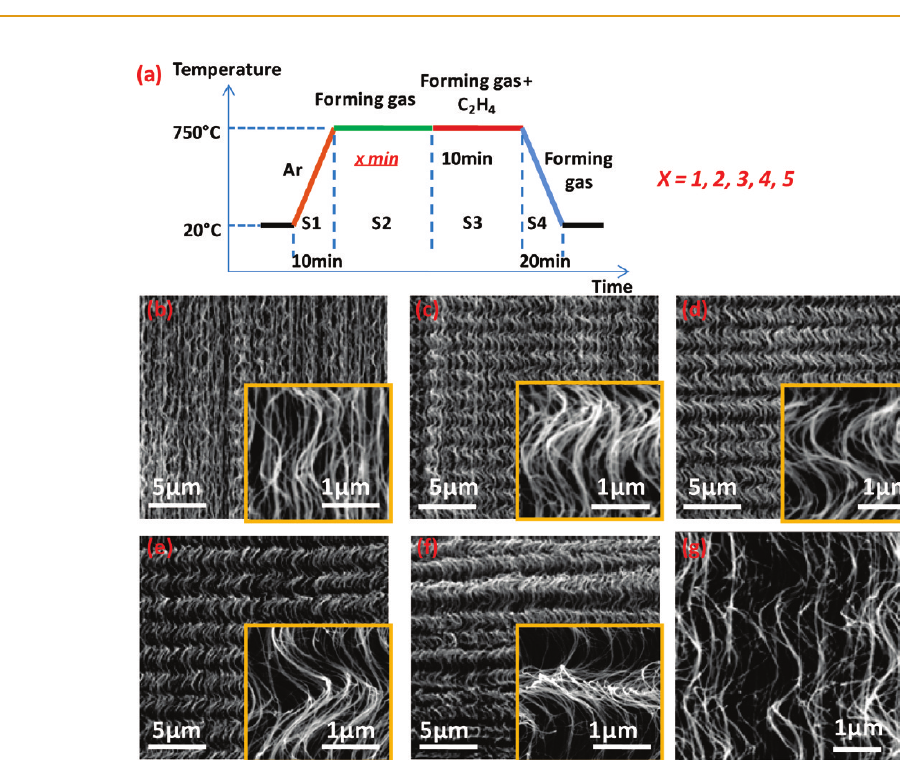
\includegraphics[width=0.92\textwidth]{figures/intro_cnt_morph_original.png}
    \caption{起伏 CNT 阵列的生长条件与典型 SEM 形貌（引自文献\cite{Zhang2009Morphology}，经裁剪）}
    \label{fig:intro_cnt_morph}
\end{figure}

\subsection{工艺参数分析、形貌关系分析与实验优化研究现状}
\ensubsection{Research Status on Morphology Relation Modeling and Experimental Optimization}

工艺参数分析、形貌关系分析与实验优化研究，主要关注如何利用已有数据刻画工艺条件与阵列形貌之间的关系，并进一步为实验设计与参数选择提供依据。围绕这一问题，数据驱动方法已在材料科学中得到广泛关注。已有研究利用模拟图像、深度学习和数据驱动方法对 CNT 阵列的结构属性与力学行为进行预测，表明工艺、结构和性能之间的映射关系在一定条件下能够通过模型学习加以近似刻画\cite{Hajilounezhad2021}。与此同时，主动学习、贝叶斯优化和闭环实验优化等方法也已被系统总结，并被广泛用于应对样本有限、实验成本高和参数空间较大的问题\cite{Lookman2019}。在 CNT 研究中，已有工作给出了利用贝叶斯优化提升生长速率的闭环实验案例\cite{Chang2020}；国内研究也开始将文献挖掘、机器学习与高通量制备相结合，用于关键生长参数分析及阵列高度、质量优化\cite{Gao2023}。进一步地，机器学习模型、自动化实验与机器人 CVD 平台的结合，也说明该方向正由单点分析逐步走向更紧密的人机协同研究模式\cite{Li2025Matter}。

总体来看，数据驱动方法已经能够在 CNT 阵列研究中用于参数分析与实验优化。然而，从本文的研究目标出发，若关键形貌标签本身缺乏稳定性，或分析结果缺少与领域机理相衔接的证据支撑，则模型输出即使在数值上具有一定效果，也难以真正转化为可靠的科研判断依据。因此，对本文而言，更合理的研究路径并不是直接追求实验优化闭环，而是先建立稳定的关键形貌表征方式，再在此基础上形成具有知识证据支撑的工艺—形貌关系分析框架。

综上，围绕 CNT 阵列的制备调控、材料知识组织、SEM 图像表征以及数据驱动分析，国内外研究都已形成一定基础。在工艺层面，已有较多关于阵列生长调控的实验认识；在知识层面，知识图谱与检索增强为多源信息组织提供了方法基础；在表征层面，CNT 图像中的部分结构信息已能够转化为定量指标；在分析层面，数据驱动方法也已能够用于参数分析与实验优化。尽管如此，从服务科研分析任务的角度看，现有工作仍未形成一条贯通工艺参数、关键形貌与生长机理的完整分析路径。前端缺少面向多源科研材料的统一知识组织方式，中间缺少稳定、可比较的关键形貌标签，后端缺少能够将工艺—形貌分析结果与机理证据衔接起来的解释机制。正因为上述三个环节尚未真正打通，工艺参数、关键形貌与生长机理之间的关系仍未得到有效连接。本文即围绕这一问题展开研究，并在后文分别从知识建模与检索增强、关键形貌自动化表征以及知识增强支持下的工艺—形貌关系分析三个方面加以展开。

\section{本文研究内容与技术路线}
\ensection{Research Content and Technical Route}

针对上述问题，本文以 CNT 阵列为研究对象，以工艺—形貌关系分析为核心任务，以知识增强为贯穿支撑手段，围绕知识组织、关键形貌表征、关系建模和结果解释展开研究，目标是构建一条贯通多源知识组织、样品级关键形貌提取、工艺—形貌关系分析与知识增强解释的分析链路。

本文的研究主要包括三个部分。第一部分研究面向碳纳米管阵列的多源知识建模与检索增强方法，处理文献、实验记录、工艺参数和图像分析结果的统一组织问题，为工艺分析、形貌解释和结果追溯提供证据支撑。第二部分研究 CNT 阵列关键形貌自动化表征方法，围绕 SEM 图像建立样品级自动化表征流程，获取取向度、平均曲率、波曲度和迂曲度等关键形貌特征，为后续关系分析提供稳定标签。第三部分研究知识增强支持下的工艺—形貌关系分析与解释方法，在知识检索结果支持下围绕 Fe 功率、Fe 厚度和退火时间等工艺变量开展统计关系分析与预测建模，并结合知识库中的机理证据对关键变量作用及预测结果进行解释。前述方法最终通过科研辅助分析平台完成集成实现与流程验证。

本文整体遵循“知识组织—关键形貌表征—关系建模—结果解释”的技术路线。先面向文献、实验记录、工艺参数表和图像分析结果构建统一知识组织框架，通过 MSFU 表示与关系约束检索获得证据链，为后续变量筛选和机理解释提供支撑。再针对 SEM 图像建立自动化关键形貌表征流程，获取取向度、平均曲率、波曲度和迂曲度等样品级结构化特征，并结合知识检索结果识别工艺—形貌关系线索，为关系建模提供稳定标签。随后，在前述形貌标签与知识线索支持下，围绕 Fe 功率、Fe 厚度和退火时间等工艺变量开展统计关系分析与预测建模。最后，将知识检索结果与样品级分析结果结合起来，对关键变量作用及预测结果进行解释，并通过科研辅助平台完成方法集成与流程验证。技术路线如图~\ref{fig:1_1} 所示。

\begin{figure}[htbp]
    \centering
    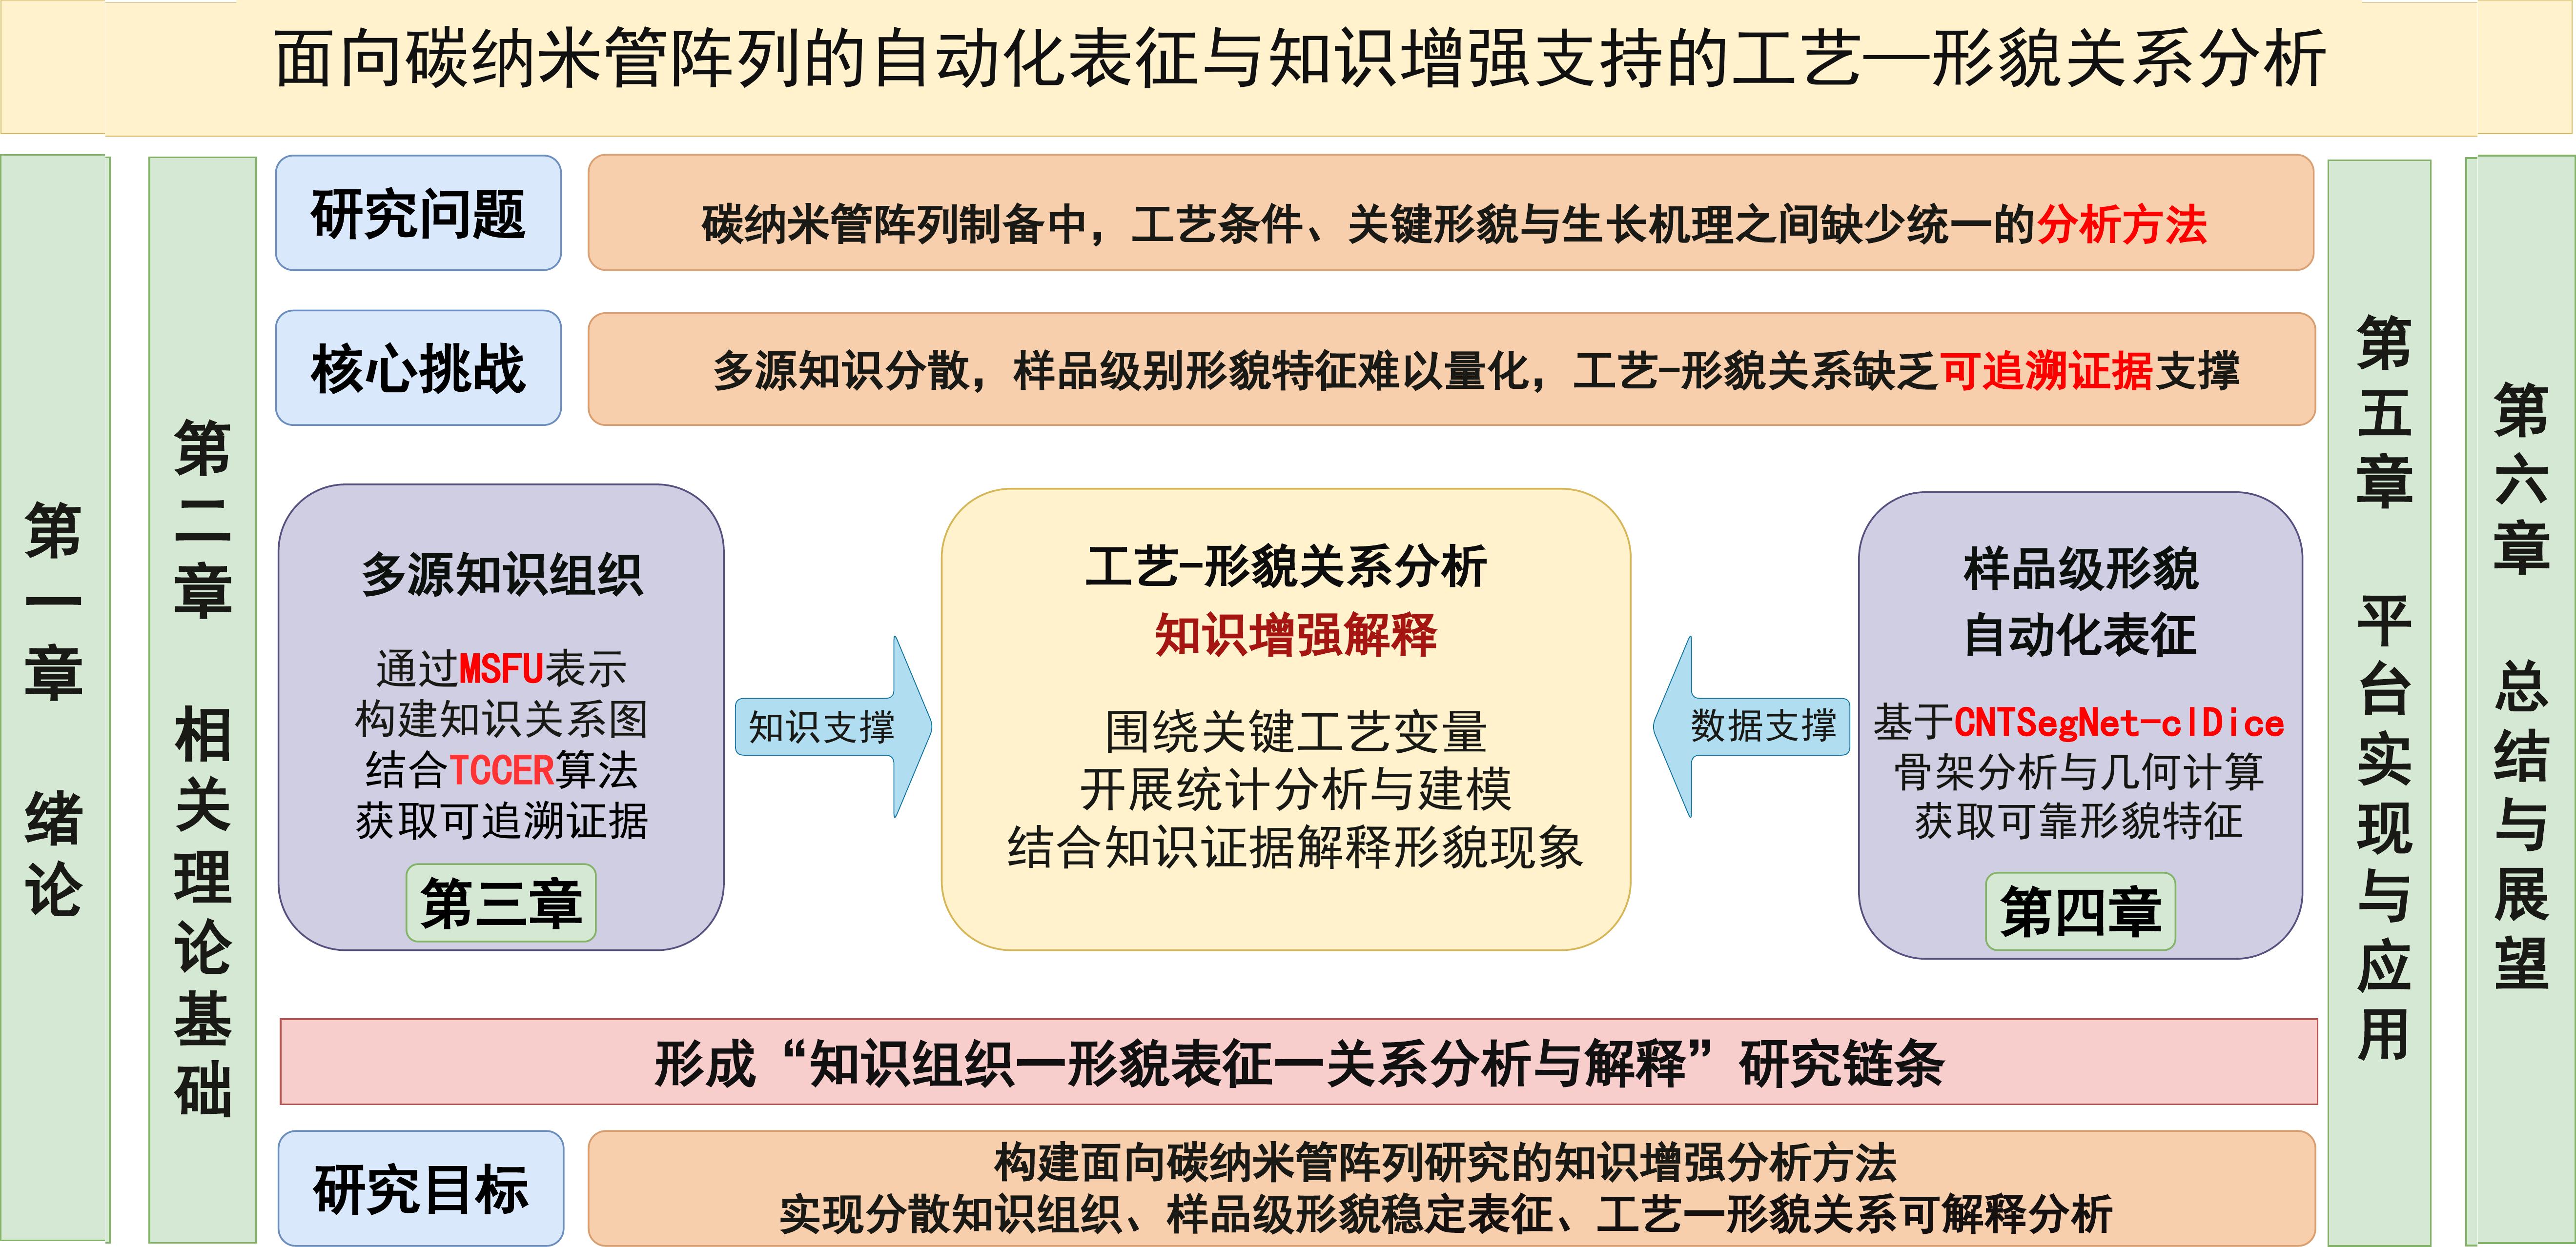
\includegraphics[width=0.98\textwidth]{figures/fig1-1-main-framework.png}
    \caption{本文技术路线图}
    \label{fig:1_1}
\end{figure}

本文的工作主要有三点特点。其一，面向 CNT 阵列科研分析任务，提出以最小语义事实单元为核心的多源知识组织方式，并构建关系约束检索方法，使工艺参数、关键形貌、生长机理与文献证据能够在同一框架下组织和调用。其二，提出服务于工艺—形貌关系分析的关键形貌自动化表征方法，围绕曲率、波曲度和迂曲度等弯曲相关特征构建样品级结构化表示，使依赖经验判断的弯曲形貌转化为可比较、可分析的结构化特征。其三，提出面向碳纳米管阵列工艺—形貌分析的知识增强解释框架，将知识库中识别出的关系线索与样品级统计分析结果结合起来，用于说明关键变量作用及其可能机制。

本文共分为六章。第一章为绪论，介绍研究背景、国内外研究现状，并说明本文的研究内容与技术路线。第二章介绍本文研究所涉及的相关理论与关键技术，包括知识组织方法、CVD 工艺机理、图像处理方法及工艺关系分析方法。第三章研究面向 CNT 阵列科研任务的知识建模与检索增强方法，解决多源知识分散、证据难以成链的问题。第四章开展 CNT 阵列 SEM 图像关键形貌自动化表征与工艺—形貌关系分析，讨论特征提取方法、参数关系分析及知识增强解释。第五章对前述方法进行系统集成，设计并实现面向 CNT 阵列研究的科研辅助分析平台，并对平台功能进行测试。第六章对全文进行总结，归纳研究成果与不足，并对后续研究方向进行展望。

围绕上述问题，本文形成了“知识组织—关键形貌表征—关系分析—结果解释”的总体技术路线。其中，第 3 章重点解决多源知识组织与证据链检索问题，第 4 章重点解决关键形貌表征与工艺—形貌关系分析问题，第 5 章对前述方法进行系统集成与验证。

\chapter{碳纳米管阵列制备工艺与知识增强方法基础}
\enchapter{Foundations of CNT Array Fabrication and Knowledge Enhancement Methods}

\section{碳纳米管阵列制备工艺基础}
\ensection{Fundamentals of CNT Array Fabrication Process}

本节介绍碳纳米管阵列制备所涉及的基本工艺与机理背景。碳纳米管阵列的形成不是单一热处理步骤的直接结果，而是催化剂薄膜演化、碳源裂解、活性碳迁移析出以及阵列内部传质共同作用的结果。不同工艺条件既决定碳纳米管能否成核和持续生长，也影响阵列的高度、密度、取向和局部形貌状态。为便于后续章节分析样品制备条件与形貌结果之间的联系，本节从碳纳米管阵列常见制备方法、催化层制备与磁控溅射基础、化学气相沉积生长过程以及关键工艺参数及其影响四个方面展开介绍。

\subsection{碳纳米管阵列常见制备方法}
\ensubsection{Common Fabrication Methods for CNT Arrays}

碳纳米管阵列的制备方法主要包括电弧放电、激光烧蚀、化学气相沉积以及部分模板辅助方法等。电弧放电和激光烧蚀依赖高能局域热源使碳蒸发并重新凝聚，通常有利于获得结晶质量较好的碳纳米管产物，但更适用于粉体制备，对基底上阵列结构的定向生长控制相对有限。模板辅助方法通过受限孔道或预设几何空间约束碳纳米管生长方向，能够在一定程度上限定局部结构形貌，但工艺灵活性和大面积连续制备能力受模板结构限制。相比之下，化学气相沉积能够在固体基底表面原位完成催化剂活化、碳源裂解、成核和连续生长过程，更适合围绕催化层、碳源和反应环境开展连续工艺调控，因此已成为碳纳米管阵列研究中最常用的制备路线\cite{Wu2025VACNTReview}。

从材料过程角度看，化学气相沉积的核心在于利用过渡金属催化剂对碳源分解、活性碳供给和碳纳米管成核进行调控。实际制备中，催化剂通常以 Fe、Co、Ni 及其合金薄膜或前驱体形式沉积在基底表面，并配合 \ce{Al2O3}、\ce{SiO2} 等缓冲层或支撑层使用。热处理过程中，连续薄膜会因表面能驱动发生去润湿和颗粒化，形成纳米尺度催化颗粒。随后，碳源分子在高温下裂解产生的活性碳物种在催化颗粒表面吸附，并通过表面扩散或体扩散进入颗粒内部，当局部碳浓度达到过饱和状态后，碳会从颗粒另一侧析出并逐步形成石墨化管壁结构\cite{Liu2021EcoMat}。这一过程中，催化剂薄膜厚度、支撑层性质和热处理条件决定颗粒尺寸、分布和界面结合状态，从而影响后续阵列的成核密度、外径分布和持续生长能力\cite{Zhang2017BufferLayer}。

\begin{table}[htbp]
    \centering
    \caption{碳纳米管阵列常见制备方法比较}
    \label{tab:ch2_cnt_fabrication_compare}
    \small
    \renewcommand{\arraystretch}{1.45}
    \setlength{\tabcolsep}{0pt}
    \begin{tabularx}{\textwidth}{@{}>{\centering\arraybackslash}m{2.2cm}>{\centering\arraybackslash}m{2.6cm}>{\centering\arraybackslash}X>{\centering\arraybackslash}m{2.2cm}@{}}
        \toprule
        方法 & 典型产物形态 & 主要特点 & 阵列制备适用性 \\
        \midrule
        电弧放电 & 粉体、团聚产物 & 产物结晶质量较高，但反应过程瞬时且难以精细调控 & 较弱 \\
        激光烧蚀 & 粉体、团簇产物 & 纯度较高，但设备要求高、连续制备能力有限 & 较弱 \\
        化学气相沉积 & 基底原位生长产物 & 便于调控催化层、碳源和气氛，适合连续生长与结构控制 & 较强 \\
        模板辅助方法 & 受限几何结构产物 & 有利于限定局部形貌，但工艺灵活性和大面积连续性受限 & 中等 \\
        \bottomrule
    \end{tabularx}
\end{table}

\subsection{催化层制备与磁控溅射基础}
\ensubsection{Catalyst Layer Preparation and Magnetron Sputtering}

对于基底固定催化剂法而言，碳纳米管阵列制备通常还包括催化层构建过程。催化层的作用不是直接给出最终形貌，而是为后续退火颗粒化和碳纳米管成核提供初始金属来源及界面条件。常见的催化层制备方式包括蒸镀、磁控溅射、原子层沉积和溶液法沉积等。其中，磁控溅射能够在较大面积基底表面获得厚度可控、均匀性较好的金属薄膜，因此在碳纳米管阵列催化层制备中应用较多\cite{Aleksanyan2023RFMagnetron}。

磁控溅射的基本原理是在真空环境下引入工作气体并形成等离子体，离子在电场作用下轰击靶材表面，使靶材原子或原子团簇溅射出来并沉积到基底表面。磁场的引入可以提高靶面附近电子密度，增强等离子体稳定性并提高沉积效率。对铁催化层而言，磁控溅射能够较稳定地调节薄膜厚度和覆盖均匀性，从而为后续热处理提供较一致的初始薄膜条件\cite{Aleksanyan2023RFMagnetron}。在随后的升温和还原过程中，这类连续薄膜会发生去润湿和颗粒化，形成催化颗粒。因而，沉积阶段形成的薄膜连续性、界面粗糙度和初始厚度会进一步影响颗粒尺寸分布、颗粒稳定性以及后续阵列成核密度\cite{Yang2016ALDThicknessCN}。

\begin{figure}[htbp]
    \centering
    \begin{tikzpicture}[
        box/.style={draw, rounded corners=2pt, align=center, font=\small, minimum height=0.95cm},
        arrow/.style={-Latex, thick}
    ]
        \node[box, minimum width=2.4cm] (target) at (0,0) {铁靶材};
        \node[box, minimum width=2.8cm] (plasma) at (3.7,0) {等离子体轰击\\与原子溅射};
        \node[box, minimum width=2.8cm] (film) at (7.7,0) {基底表面\\铁薄膜沉积};
        \node[box, minimum width=2.9cm] (anneal) at (11.9,0) {退火后去润湿\\与颗粒化};
        \draw[arrow] (target) -- (plasma);
        \draw[arrow] (plasma) -- (film);
        \draw[arrow] (film) -- (anneal);

        \draw[fill=gray!20] (6.9,-1.9) rectangle (8.5,-1.65);
        \draw[fill=gray!55] (6.95,-1.65) rectangle (8.45,-1.48);
        \node[font=\small] at (7.7,-2.25) {连续薄膜};

        \draw[fill=gray!20] (11.1,-1.9) rectangle (12.7,-1.65);
        \foreach \x in {11.35,11.8,12.25,12.55} {
            \draw[fill=gray!55] (\x,-1.5) circle (0.11);
        }
        \node[font=\small] at (11.9,-2.25) {催化颗粒};
    \end{tikzpicture}
    \caption{磁控溅射催化层形成及后续颗粒化过程示意}
    \label{fig:ch2_sputter_catalyst_schematic}
\end{figure}

\subsection{碳纳米管阵列CVD生长过程}
\ensubsection{CVD Growth Process of CNT Arrays}

化学气相沉积制备碳纳米管阵列的过程通常包括催化剂活化、碳源裂解、活性碳迁移析出以及碳纳米管持续生长等阶段\cite{Liu2021EcoMat}。在生长初期，沉积在基底表面的催化剂薄膜会在热处理和还原气氛作用下重排并形成纳米颗粒，这些颗粒的尺寸、分布和活性状态决定了后续成核条件。碳源进入反应区后发生裂解，形成的活性碳物种在催化颗粒表面吸附，并沿颗粒表面或内部向低化学势区域迁移，最终在颗粒边缘或背离碳源的一侧析出，逐步卷曲形成石墨化管壁结构。随着反应持续进行，碳源裂解效率、活性碳迁移速率以及催化剂失活速度会共同影响阵列的生长速率和持续时间。

按照催化颗粒与基底之间结合状态的不同，碳纳米管生长通常可以分为根部生长和顶端生长两种模式。当催化颗粒与基底结合较强时，颗粒更容易停留在基底表面，碳纳米管自颗粒上方向外延伸，对应根部生长模式；当催化颗粒与基底结合较弱时，生长过程中颗粒可能被抬升至管顶，对应顶端生长模式\cite{Liu2021EcoMat}。对于垂直排列阵列而言，催化颗粒与支撑层之间的界面作用、颗粒润湿行为以及阵列内部范德华相互作用会共同影响生长模式及其稳定性\cite{Zhang2017BufferLayer}。随着阵列高度增加，气相反应物从阵列顶部向底部传输的距离不断增大，反应物浓度梯度、催化剂中毒、颗粒粗化以及无定形碳沉积等因素会逐渐积累，并最终导致生长减速甚至终止\cite{He2011LongAlignedCN}。因此，碳纳米管阵列的形成本质上是催化剂演化、气相供给和阵列内部传质共同耦合的过程。

\begin{figure}[htbp]
    \centering
    \begin{tikzpicture}[
        box/.style={draw, rounded corners=2pt, align=center, font=\small, minimum height=0.9cm},
        arrow/.style={-Latex, thick}
    ]
        \node[box, minimum width=2.3cm] (film) at (0,0) {催化剂薄膜};
        \node[box, minimum width=2.5cm] (particle) at (3.4,0) {退火后纳米颗粒};
        \node[box, minimum width=2.7cm] (adsorb) at (7.2,0) {碳源裂解与\\活性碳吸附};
        \node[box, minimum width=2.7cm] (grow) at (11.1,0) {成核、生长与\\阵列延伸};
        \draw[arrow] (film) -- (particle);
        \draw[arrow] (particle) -- (adsorb);
        \draw[arrow] (adsorb) -- (grow);

        \draw[fill=gray!20] (-0.9,-2.0) rectangle (1.0,-1.75);
        \draw[fill=gray!50] (-0.1,-1.75) circle (0.22);
        \draw[thick] (-0.1,-1.53) -- (-0.1,-0.7);
        \node[font=\small] at (0,-2.35) {根部生长};

        \draw[fill=gray!20] (2.8,-2.0) rectangle (4.7,-1.75);
        \draw[thick] (3.75,-1.75) -- (3.75,-0.95);
        \draw[fill=gray!50] (3.75,-0.73) circle (0.22);
        \node[font=\small] at (3.75,-2.35) {顶端生长};

        \node[font=\small, align=center] at (7.2,-1.5) {支撑层和基底影响颗粒稳定性\\碳源供给影响持续生长能力};
    \end{tikzpicture}
    \caption{碳纳米管阵列 CVD 生长过程与典型生长模式示意}
    \label{fig:ch2_cvd_growth_schematic}
\end{figure}

\subsection{关键工艺参数及其形貌影响}
\ensubsection{Key Process Parameters and Their Effects on Morphology}

在碳纳米管阵列 CVD 生长过程中，温度、催化剂与基底条件、碳源及载气组成、气体流量和生长时间是较为常见的关键工艺参数\cite{Szabo2017}。这些参数并不直接作用于最终形貌，而是先作用于催化剂演化、碳源裂解、活性碳迁移和阵列内部传质，再进一步反映为阵列高度、密度和取向状态的差异。其中，温度直接影响碳源裂解效率、催化剂活性和碳扩散速率。温度过低时，碳源裂解不足，活性碳供给有限，阵列难以快速生长；温度过高时，虽然裂解和扩散过程会增强，但催化颗粒也更容易粗化和失活，从而降低阵列均匀性和持续生长能力。催化剂类型、厚度、颗粒尺寸及其与基底的匹配关系会影响成核行为和后续阵列生长稳定性。一般而言，催化层越厚，退火后形成的催化颗粒尺寸越大，对应生成的碳纳米管外径和壁数也往往增大，但阵列密度和高度可能下降\cite{Yang2016ALDThicknessCN}。

碳源、载气和辅助气体的配比关系到活性碳供给、表面反应环境及副反应抑制效果。以乙炔、乙烯、甲烷和二甲苯等为代表的碳源，其裂解活性和副产物组成存在差异，因此对应的活性碳浓度、生长速率和成碳倾向也不同。氢气常用于维持还原气氛并抑制部分无定形碳沉积，水蒸气、氧等微量氧化性组分则可能在一定范围内清除催化剂表面的无定形碳，从而延长催化剂寿命\cite{Hata2004}，但含量过高又可能加速催化剂腐蚀与失活\cite{Liu2021EcoMat}。气体流量和反应压力进一步决定反应物在阵列上方和阵列内部的传输条件。流量不足会限制碳源供应，流量过高则可能缩短有效停留时间并扰动反应区稳定性；当阵列逐渐增高时，底部区域的反应物补给和副产物排出还会受到更强的传质限制。

生长时间主要影响阵列生长阶段的累积过程。随着生长时间延长，阵列高度通常先快速增加，再逐渐进入减速阶段，最终因催化剂失活或传质受限而趋于停止\cite{Bulyarskiy2020}。因此，这些工艺参数通常不是彼此独立起作用的，而是通过影响催化剂演化、表面反应和质量传输过程共同作用于阵列结构。

在较宽的工艺范围内，生长速率对温度的响应常可用 Arrhenius 关系近似描述，其一般形式可写为
\begin{equation}
    k = A \exp\left(-\frac{E_{\mathrm{a}}}{RT}\right)
\end{equation}
其中，$k$ 表示表观反应速率常数，$A$ 为指前因子，$E_{\mathrm{a}}$ 为表观活化能，$R$ 为气体常数，$T$ 为绝对温度。该式反映了温度对碳源裂解和表面反应速率的基础影响。在实际阵列生长中，观测到的整体生长速率还会同时受到催化剂失活和阵列内部传质过程的制约\cite{Liu2021EcoMat}。

这些工艺条件会在阵列高度、取向状态、覆盖程度、直径分布以及局部波曲形态等方面留下明显差异\cite{Bulyarskiy2020}。例如，催化层厚度变化会影响催化颗粒尺寸，从而进一步改变阵列外径、壁数和高度\cite{Yang2016ALDThicknessCN}；生长温度和气氛条件变化会影响阵列的垂直排列状态和持续生长能力\cite{Liu2021EcoMat}；当生长速率、催化剂稳定性和阵列内部应力状态发生变化时，阵列还可能由较规整的森林状结构转向更明显的起伏、弯曲和波曲形态\cite{Zhang2009Morphology}。因此，工艺参数与关键形貌之间的关系并不是简单的一一对应关系，而是需要结合催化剂演化、表面反应和传质过程加以理解。这也构成了后续关键形貌提取和工艺关联分析的工艺背景。

\begin{figure}[htbp]
    \centering
    \begin{tikzpicture}[
        node distance=0.7cm,
        box/.style={draw, rounded corners=2pt, align=center, font=\small, minimum height=0.95cm},
        arrow/.style={-Latex, thick}
    ]
        \node[box, text width=3.2cm] (param) {温度、气体流量、\\催化剂条件、生长时间};
        \node[box, right=1.0cm of param, text width=3.1cm] (mech) {裂解与扩散、催化剂活化/失活、\\阵列内部应力演化};
        \node[box, right=1.0cm of mech, text width=3.2cm] (morph) {高度、取向度、\\曲率、覆盖密度};
        \draw[arrow] (param) -- (mech);
        \draw[arrow] (mech) -- (morph);
    \end{tikzpicture}
    \caption{工艺参数、过程机理与关键形貌之间的一般关系}
    \label{fig:ch2_process_morphology_relation}
\end{figure}

\section{知识增强方法基础}
\ensection{Fundamentals of Knowledge Enhancement Methods}

本节介绍第三章知识建模与检索分析所依托的基本方法。相关任务既涉及专业术语与条件约束，也涉及对象关系与来源依据，因此需要同时考虑语言模型、知识组织和检索调用三个层面的技术基础。本节从 Transformer 与大语言模型原理、大语言模型领域适配与知识增强原理、图结构知识组织原理以及检索增强与证据组织原理四个方面展开。

\subsection{Transformer与大语言模型基础原理}
\ensubsection{Fundamental Principles of Transformer and Large Language Models}

当前主流大语言模型通常建立在 Transformer 架构基础之上\cite{52vaswani2017attention}。Transformer 主要由词元嵌入、位置编码、多头自注意力、前馈网络、残差连接和层归一化等模块组成，其核心是通过自注意力机制刻画序列内部不同位置之间的相关性。自注意力的一般形式可写为
\begin{equation}
    \mathrm{Attention}(Q,K,V)=\mathrm{softmax}\left(\frac{QK^{\top}}{\sqrt{d_k}}\right)V
\end{equation}
其中，$Q$、$K$ 和 $V$ 分别表示查询矩阵、键矩阵和值矩阵，$d_k$ 表示键向量维度。该式表明模型会依据当前位置与上下文各位置之间的相关性，对输入信息进行加权聚合。相较于传统循环结构，Transformer 更适合处理长距离依赖较强的文本序列。

在单个 Transformer 块内，多头自注意力和前馈网络通常按残差方式顺序堆叠，其计算过程可写为
\begin{equation}
    \tilde{H}=\mathrm{LayerNorm}\bigl(H+\mathrm{MHAtt}(H)\bigr),\qquad
    H^{\prime}=\mathrm{LayerNorm}\bigl(\tilde{H}+\mathrm{FFN}(\tilde{H})\bigr)
\end{equation}
其中，$H$ 表示输入表示，$\mathrm{MHAtt}(\cdot)$ 表示多头自注意力，$\mathrm{FFN}(\cdot)$ 表示位置前馈网络。该式反映了 Transformer 通过注意力聚合和非线性变换逐层更新序列表征的过程。

在此基础上，大语言模型通过大规模语料预训练学习文本序列中的条件概率关系，使模型能够根据已有上下文逐步生成后续词元。其自回归建模形式通常可写为
\begin{equation}
    P(x)=\prod_{t=1}^{T}P(x_t\mid x_{<t})
\end{equation}
式中，$x_t$ 表示第 $t$ 个词元，$x_{<t}$ 表示当前位置之前的上下文。该式说明模型输出直接受输入语境和任务指令影响。图~\ref{fig:ch2_transformer_ref} 给出了 Vaswani 等\cite{52vaswani2017attention} 原始论文中的 Transformer 整体结构参考图。

\begin{figure}[htbp]
    \centering
    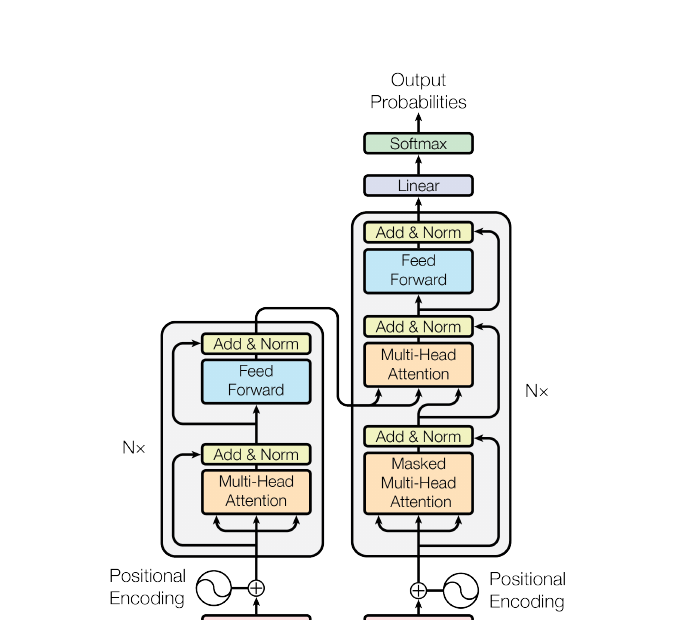
\includegraphics[width=0.64\textwidth]{figures/chapter2/refs/fig_transformer_ref.png}
    \caption{Transformer基本结构参考图，引自文献\cite{52vaswani2017attention}}
    \label{fig:ch2_transformer_ref}
\end{figure}

\subsection{大语言模型领域适配与知识增强原理}
\ensubsection{Principles of Domain Adaptation and Knowledge Enhancement for Large Language Models}

当大语言模型用于专业领域分析任务时，模型输出通常需要同时满足术语约束、结构约束和依据约束。若缺少这些约束，模型虽然能够生成表面连贯的回答，但结果未必稳定可靠\cite{Choi2024,Jiang2025}。

在不改变模型参数的前提下，知识增强通常通过输入侧注入任务约束、示例信息和外部知识来实现。设原始问题为 $x$，任务指令与格式约束为 $p$，示例集合为 $E$，外部知识上下文为 $K$，则增强后的模型输出可抽象表示为
\begin{equation}
    y=\mathcal{M}_{\theta}(x,p,E,K)
\end{equation}
其中，$\mathcal{M}_{\theta}$ 表示参数固定的大语言模型，$p$ 用于约束回答任务和输出形式，$E$ 用于提供少样本示例，$K$ 用于补充术语解释、条件范围和结论依据。该式表明，知识增强的核心是在模型输入中显式加入任务所需的结构约束和外部知识。

在这一机制下，提示词约束、少样本示例和结构化输出要求主要用于控制模型的输入输出形式\cite{Polak2024}。当任务涉及术语解释、条件比对和结论依据说明时，还需要接入外部知识，以补充模型参数中难以显式更新和直接追溯的内容\cite{Mostafa2024}。因此，大语言模型更适合承担知识增强链路中的语言处理与生成任务。

在专业领域应用中，常见的模型适配路径主要包括领域微调和检索增强。前者主要通过在特定任务或领域语料上继续训练提升模型适应性，后者主要通过外部知识检索补充推理依据\cite{Soudani2024,lewis2020rag,Mostafa2024}。对于知识更新频繁、条件约束较多且需要证据支撑的科研分析任务，检索增强通常更适合与后续的结构化知识表示和检索链路配合使用。

\subsection{图结构知识组织基本原理}
\ensubsection{Basic Principles of Graph-based Knowledge Organization}

在科研分析任务中，知识对象往往不仅是孤立文本片段，还包括对象、条件、结果和机理概念之间的对应关系。若仅以文本段落或向量表示保存相关信息，虽然可以保留局部语义，但对象之间的关系结构、条件范围和来源依据较难显式表达。为此，通常需要进一步引入结构化知识表示，对多源信息进行统一组织\cite{Statt2023,Venugopal2024}。

图结构知识表示能够较好地组织对象、条件、结果和解释之间的关系。其基本思想是将知识表示为由节点和边组成的网络结构，其中节点用于表示对象单元，边用于描述对象之间的关联关系。其一般形式可写为
\begin{equation}
    \mathcal{G}=(\mathcal{V},\mathcal{E},\mathcal{A})
\end{equation}
其中，$\mathcal{V}$ 表示节点集合，$\mathcal{E}$ 表示边集合，$\mathcal{A}$ 表示与节点或边相关的属性信息。节点可用于表示文献、样品、工艺参数、形貌指标或机理概念等对象，边用于表示对象之间的对应、作用或来源关系，属性则用于保留条件范围、单位、时间信息和证据标识等内容。

在局部关系层面，图结构中的单条知识关系还可抽象写为
\begin{equation}
    \tau_{ij}=\bigl(v_i,r_{ij},v_j,a_{ij}\bigr)
\end{equation}
其中，$v_i$ 和 $v_j$ 分别表示起点节点和终点节点，$r_{ij}$ 表示关系类型，$a_{ij}$ 表示与该关系相关的属性集合。$a_{ij}$ 通常包含条件范围、来源标识、时间信息和证据编号等内容。采用这种表示方式后，知识对象之间的关系不仅能够被显式保存，还能进一步保留关系成立的适用条件和来源依据。

相较于纯文本块或单一向量表示，图结构不仅保留内容本身，还能够显式表示对象关系、条件范围、证据来源和上下位关联，因此更适合承担知识组织与结构保存任务。这一组织思想与科研数据可追溯、可复用的基本要求是一致的\cite{Wilkinson2016FAIR,Lebo2013PROVO}。图~\ref{fig:ch2_kg_ref} 给出了知识图谱原始参考图，其节点、关系和属性的表达方式可为后续中文化改绘提供参照\cite{Hogan2021KG}。

\begin{figure}[htbp]
    \centering
    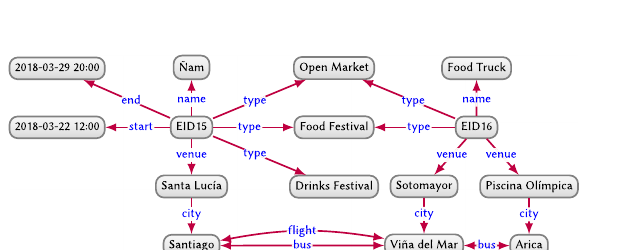
\includegraphics[width=0.78\textwidth]{figures/chapter2/refs/fig_kg_ref_hogan.png}
    \caption{知识图谱基本结构参考图，引自文献\cite{Hogan2021KG}}
    \label{fig:ch2_kg_ref}
\end{figure}

\subsection{检索增强与证据组织基本原理}
\ensubsection{Basic Principles of Retrieval Augmentation and Evidence Organization}

检索增强的基本思想，是在生成之前先从外部知识源中检索相关信息，再将检索结果与用户问题一并输入模型，从而提高回答的针对性和可信度\cite{lewis2020rag}。在科研分析任务中，检索返回的结果不仅需要相关，还需要能够支撑后续对象判定、条件比对和结果说明。图~\ref{fig:ch2_rag_ref} 给出了 Lewis 等\cite{lewis2020rag} 在原始论文中提出的 RAG 结构参考图，其展示了查询编码器、检索器、文档索引和生成器之间的连接关系。

\begin{figure}[htbp]
    \centering
    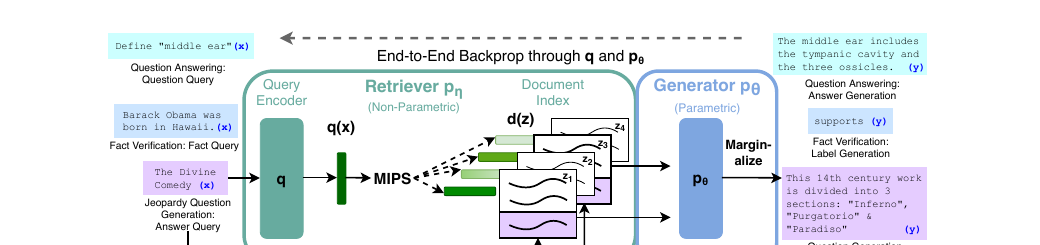
\includegraphics[width=\textwidth]{figures/chapter2/refs/fig_rag_ref.png}
    \caption{RAG基本结构参考图，引自文献\cite{lewis2020rag}}
    \label{fig:ch2_rag_ref}
\end{figure}

在科研文本检索任务中，候选条目通常需要先转化为可以计算相似度的表示形式。传统稀疏检索主要依托倒排索引和词项权重完成候选召回，较有利于保持专业术语、参数符号和条件短语的精确匹配，但对语义近邻和跨表述变体的覆盖相对有限\cite{Mostafa2024}。以 BM25 为代表的稀疏检索评分形式通常可写为\cite{Robertson2009BM25}
\begin{equation}
    S_{\mathrm{sparse}}(q,d)=\sum_{t\in q}\mathrm{IDF}(t)\cdot
    \frac{f(t,d)(k_1+1)}{f(t,d)+k_1\left(1-b+b\frac{|d|}{\mathrm{avgdl}}\right)}
\end{equation}
其中，$f(t,d)$ 表示词项 $t$ 在候选条目 $d$ 中的出现频次，$|d|$ 表示条目长度，$\mathrm{avgdl}$ 表示候选集合中的平均长度，$k_1$ 和 $b$ 为控制词频饱和和长度归一化的参数。该式说明稀疏检索主要依赖词项匹配程度和文档统计特征完成候选排序。稠密检索则通过编码模型将查询和候选条目映射为向量表示，再利用向量空间中的距离或相似度衡量二者的语义接近程度。句向量模型和双编码器结构是较常见的技术形式，其优点在于能够将不同表述但语义相近的内容映射到相邻空间位置\cite{Reimers2019SentenceBERT}。

对查询 $q$ 和候选条目 $d$ 而言，稠密表示的一般形式可写为
\begin{equation}
    \mathbf{z}_q=f(q),\qquad \mathbf{z}_d=f(d)
\end{equation}
其中，$f(\cdot)$ 表示向量编码函数，$\mathbf{z}_q$ 和 $\mathbf{z}_d$ 分别表示查询与候选条目的向量表示。对应的语义相似度通常可写为
\begin{equation}
    S_{\mathrm{dense}}(q,d)=\cos(\mathbf{z}_q,\mathbf{z}_d)=\frac{\mathbf{z}_q^{\top}\mathbf{z}_d}{\lVert \mathbf{z}_q\rVert \lVert \mathbf{z}_d\rVert}
\end{equation}
该式反映了稠密检索通过向量方向相近程度衡量语义相似性的基本思想。

在科研任务中，研究者关心的往往不是单一事实，而是条件、现象和解释之间的关联过程。仅依赖关键词检索容易忽略语义近邻，仅依赖向量检索又可能弱化条件约束和专业术语的精确匹配，因此混合检索逐渐成为更常见的技术路线\cite{Mostafa2024}。在混合检索阶段，稀疏检索结果与稠密检索结果通常采用加权融合方式共同参与排序，其一般形式可写为
\begin{equation}
    S_{\mathrm{hyb}}(q,d)=\alpha S_{\mathrm{sparse}}(q,d)+(1-\alpha)S_{\mathrm{dense}}(q,d)
\end{equation}
其中，$S_{\mathrm{sparse}}$ 和 $S_{\mathrm{dense}}$ 分别对应关键词匹配得分与语义相似度得分，$\alpha$ 用于控制两类信息在候选排序中的相对权重。该式表明，混合检索的核心在于同时保留术语精确匹配能力和语义召回能力。

证据组织关注的是如何将检索结果按对象、条件、来源和关系进行重新整理，使输出内容能够直接支撑后续分析判断。单条证据可进一步抽象表示为
\begin{equation}
    e_i=(o_i,c_i,r_i,\pi_i)
\end{equation}
其中，$o_i$ 表示证据对应的对象单元，$c_i$ 表示适用条件，$r_i$ 表示核心关系或判断，$\pi_i$ 表示来源与定位信息。证据不仅要相关，还应能够回溯其来源、生成过程和适用条件\cite{Soudani2024}。因此，检索增强通常还需要与前述图结构知识表示配合使用，才能将返回结果整理为可分析、可追溯和可复用的知识依据。

\section{小结}
\ensection{Summary}

本章围绕后续章节所需的两类基础展开，即碳纳米管阵列制备工艺基础和知识增强方法基础。前一部分说明了碳纳米管阵列常见制备路线、CVD 生长过程以及关键工艺参数与形貌之间的联系，为后续工艺变量分析提供过程背景。后一部分介绍了 Transformer 与大语言模型原理、大语言模型领域适配与知识增强原理、图结构知识组织原理以及检索增强与证据组织原理，为第三章的多源知识建模与证据链检索方法提供支撑。通过这些准备，后续章节中的知识增强分析和工艺—形貌关系研究能够更自然地衔接起来。

\chapter{面向碳纳米管阵列研究的知识建模与检索增强方法}
\enchapter{Knowledge Modeling and Retrieval Augmentation Methods for Carbon Nanotube Array Research}
\label{chap:knowledge_method}

\section{引言}
\ensection{Introduction}

碳纳米管阵列研究涉及工艺参数调控、形貌特征表征、生长机理分析与材料性能评估等多个环节，不同环节之间存在明显的条件依赖关系与因果传递关系。随着大语言模型和检索增强生成技术的发展，利用外部知识支撑科研分析成为可能。然而，在碳纳米管阵列这类专业性强、机理链条复杂、实验条件敏感的研究场景中，通用文本块式检索增强方法仍存在明显局限：其通常以固定长度文本片段作为基本检索单元，难以显式保留“工艺参数—生长机理—形貌特征—材料性能”之间的局部科研事实结构，也难以满足面向条件约束和关系约束的精确检索需求。由此，在进行形貌解释、规律归纳或结果分析时，模型容易检索到语义相关但结构割裂的证据片段，从而影响分析结果的准确性、可追溯性与可解释性。

针对上述问题，本章提出一种面向碳纳米管阵列研究的知识建模与检索增强方法。本章不追求构建复杂的图学习模型，而是以最小语义事实单元为基础，通过轻量级领域关系结构和任务约束检索机制，实现面向科研分析任务的链式证据组织与调用。具体而言，本章的方法主线包括以下三个环节：
\begin{enumerate}
    \item \textbf{多源知识规范化与层次化切分。}面向学术文献、实验记录、工艺参数表、结构化实验数据及图像分析结果，构建多源知识规范化处理流程，并设计面向科研事实的层次化切分方法，将异构原始知识转化为统一、可关联的候选知识片段。
    \item \textbf{科研事实表示与领域关系建模。}提出最小语义事实单元表示方法，并建立核心对象、关系类型与约束规则组成的轻量级领域关系结构，实现对“工艺参数—生长机理—形貌特征—材料性能”等关键科研关系的结构化表达。
    \item \textbf{面向科研任务的检索增强算法。}在上述知识表示基础上，设计面向科研任务的检索增强方法，通过混合召回、关系约束扩展与路径重排序，生成支持科研分析与结果解释的链式证据集合。
\end{enumerate}

在此基础上，第 3.4 节进一步给出面向上述方法的评测设计，用于验证知识单元建模与链式证据检索的有效性。需要说明的是，本章输出的并不是最终科研结论，而是为后续结果解释与规律归纳提供证据基础。图~\ref{fig:3_1} 给出了本章方法的整体框架，其主要包括知识规范化与事实单元构建、关系约束检索与证据生成，以及对应的评测安排三个层次。

\begin{figure}[htbp]
    \centering
    \includegraphics[width=0.95\textwidth]{figures/3.1.png}
    \caption{面向碳纳米管阵列研究的知识建模与检索增强框架}
    \label{fig:3_1}
\end{figure}

\section{面向碳纳米管阵列研究的知识单元建模方法}
\ensection{Knowledge Unit Modeling Method for Carbon Nanotube Array Research}

为支撑后续关系约束检索与证据组织任务，需要将来源分散、形式异构且语义粒度不一致的原始知识转化为统一、可关联的结构化表示。针对碳纳米管阵列研究中学术文献、实验记录、工艺参数表、结构化数据库及图像表征结果并存的特点，本文围绕多源知识规范化、面向科研事实的层次化切分、最小语义事实单元构建以及核心对象—关系规则建模四个方面开展知识表示研究。规范化处理的目标不是保留所有原始格式细节，而是将不同来源知识统一映射为后续切分、抽取与索引所需的中间表示。

\subsection{多源知识规范化处理}
\ensubsection{Normalized Processing of Multi-source Knowledge}

碳纳米管阵列研究中的原始知识来源主要包括学术文献、实验记录与工艺参数表、结构化实验数据库以及图像表征结果。由于不同来源数据在文件格式、字段组织方式和语义表达粒度上存在显著差异，若直接作为后续知识建模的输入，容易导致同类信息表示不一致、样品标识无法对齐以及上下文语义缺失等问题。为此，本文设计一套面向多源异构知识的规范化处理流程，将不同来源知识统一转换为结构一致、字段清晰的标准化中间表示。

设原始多源知识集合为
\begin{equation}
    D=\{d_k\}_{k=1}^{N}
\end{equation}
其中，$d_k$ 表示第 $k$ 个原始知识对象。本文通过规范化映射函数 $F_{\mathrm{norm}}(\cdot)$ 将原始知识对象统一转换为规范化知识对象：
\begin{equation}
    \tilde{d}_k=F_{\mathrm{norm}}(d_k)
\end{equation}
其中，$\tilde{d}_k$ 表示经过格式清洗、字段对齐和标识统一后的规范化对象。为明确规范化阶段的统一输出形式，本文进一步将任一规范化对象表示为
\begin{equation}
    \tilde{d}_k=(x_k,\, m_k,\, f_k)
\end{equation}
其中，$x_k$ 表示可供后续切分的规范化文本主体；$m_k$ 表示来源标识、样品编号、来源类型、时间或年份等元数据；$f_k$ 表示已经完成字段对齐的结构化内容，如工艺参数、形貌指标、性能指标和机理术语等。无论原始来源是文献段落、实验记录、参数表还是图像分析结果，规范化阶段均输出上述统一结构，从而为后续切分、事实单元构建与索引组织提供一致输入。

针对不同类型的数据源，本文采用差异化但口径统一的规范化处理策略。学术文献以段落或句群为基本处理单元，重点完成版式去噪、术语归一化和来源信息保留；实验记录与工艺参数表以样品编号或批次编号为主键，重点完成参数项、单位和值的统一映射；结构化实验数据库以记录行为规范化对象，重点完成字段对齐、缺失值处理和主键关联；图像表征结果则直接以量化后的形貌指标作为结构化输入。四类数据源的具体处理口径如表~\ref{tab:3_1_norm_sources} 所示。

\begin{table}[htbp]
    \centering
    \caption{多源知识规范化对象及处理口径}
    \label{tab:3_1_norm_sources}
    \renewcommand{\arraystretch}{1.3}
    \setlength{\tabcolsep}{5pt}
    \begin{tabular}{p{2.4cm} p{2.6cm} p{4.5cm} p{4.0cm}}
        \toprule
        \textbf{数据源类型} & \textbf{基本处理对象} & \textbf{规范化动作} & \textbf{统一输出重点} \\
        \midrule
        学术文献 & 段落或句群 & 版式去噪、术语归一化、章节位置保留、参考信息抽取 & 文本主体 $x_k$ 及文献来源元数据 $m_k$ \\
        \midrule
        实验记录与工艺参数表 & 样品编号或批次编号对应记录 & 参数项对齐、单位统一、数值映射、记录位置保留 & 结构化参数字段 $f_k$ 及样品级元数据 $m_k$ \\
        \midrule
        结构化实验数据库 & 单条记录行 & 字段对齐、缺失值处理、主键关联、跨表整合 & 围绕样品实体组织的结构化字段 $f_k$ \\
        \midrule
        图像表征结果 & 已量化的形貌指标记录 & 样品绑定、来源绑定、表征条件绑定 & 取向度、平均曲率、覆盖密度、直径分布等字段写入 $f_k$ \\
        \bottomrule
    \end{tabular}
\end{table}

多源异构知识规范化处理流程如图~\ref{fig:3_2_norm_flow} 所示。通过上述处理，原本分散且异构的多源知识被转换为统一的规范化对象集合，为后续层次化切分、跨源样品对齐和关系抽取提供了一致输入。

\begin{figure}[H]
    \centering
    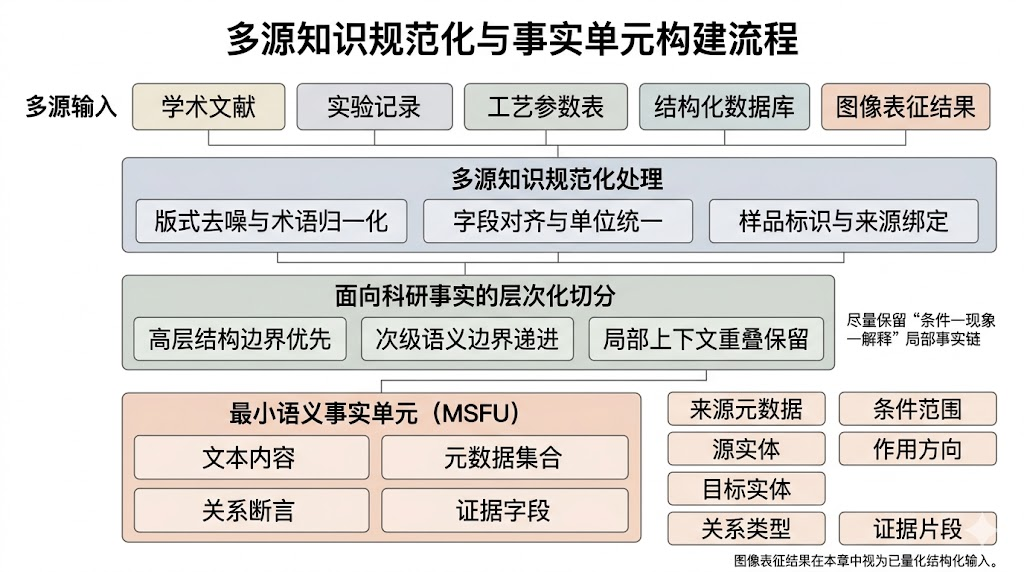
\includegraphics[width=0.92\textwidth]{figures/3.2.jpg}
    \caption{多源知识规范化与事实单元构建流程示意图}
    \label{fig:3_2_norm_flow}
\end{figure}

\subsection{面向科研事实的层次化切分方法}
\ensubsection{Hierarchical Segmentation Method Based on Scientific Facts}

在完成多源知识规范化处理后，需要将长文本转换为适合信息抽取的候选片段。对于碳纳米管阵列研究语料而言，单个文本段落中往往同时包含工艺条件、实验现象及机理解释等多类信息。若采用固定长度或滑动窗口的普通切分方式，容易破坏“条件—现象—解释”这一局部科研事实链条。为此，本文设计了一种面向科研事实的层次化切分方法，其目标是在满足模型处理长度约束的同时，尽可能保留局部事实表达的完整性。

设规范化后的知识对象 $\tilde{d}_k$ 对应文本内容为 $x_k$，本文定义分段映射函数 $F_{\mathrm{seg}}(\cdot)$，将其转换为候选片段集合：
\begin{equation}
    C_k=F_{\mathrm{seg}}(x_k)=\{c_{k,j}\}_{j=1}^{M_k}
\end{equation}
其中，$c_{k,j}$ 表示从第 $k$ 个知识对象中切分得到的第 $j$ 个候选片段，$M_k$ 表示该对象切分后的片段总数。与仅以长度为依据的滑动窗口切分不同，本文优先依据科研事实边界进行分段，以尽量保留“条件—现象—解释”的局部表达完整性。

该方法遵循“高层结构边界优先、次级语义边界递进、局部上下文重叠保留”的原则。首先，优先依据段落换行、小节标题、实验步骤和参数列表等高优先级结构边界进行初始划分，以避免截断完整论述单元。其次，当初步得到的片段长度仍超过预设阈值时，再沿句号、分号及并列参数项边界进行递归细分，使片段在满足长度约束的同时保持局部语义连续性。最后，为减弱硬性切分对指代关系和上下文依赖的影响，在相邻片段之间保留局部重叠窗口。设单个片段允许的最大长度为 $L_{\max}$，相邻片段之间保留的重叠长度为 $r$，则有：
\begin{equation}
    L(c_{k,j})\leq L_{\max}
\end{equation}
\begin{equation}
    c'_{k,j}= \mathrm{tail}_{r}(c_{k,j-1}) \oplus c_{k,j}
\end{equation}
其中，$\mathrm{tail}_{r}(\cdot)$ 表示取前一片段末尾长度为 $r$ 的文本，$\oplus$ 表示文本拼接操作。参数 $L_{\max}$ 由后续编码模型的输入长度约束与单条科研事实的完整表达需求共同确定，用于避免片段过长而影响抽取稳定性；参数 $r$ 用于保留相邻片段之间的局部上下文，通常取能够覆盖条件短语、指代成分或句间承接信息的最小窗口。为避免后文记号切换造成歧义，下文中凡指经过重叠增强后的最终片段，均统一记作 $c_{k,j}$。

与传统固定长度切分相比，该方法生成的片段不再是彼此割裂的文本块，而是保留局部科研逻辑结构的候选表达单元，并作为后续最小语义事实单元构建与关系抽取的稳定输入。

\subsection{最小语义事实单元表示}
\ensubsection{Representation of Minimum Semantic Fact Unit}

在获得保留局部逻辑的候选片段后，仍需进一步将非结构化文本转化为可检索、可关联的科研事实表示。传统文本片段主要支持基于关键词或向量相似度的检索方式，难以显式表达知识内部的对象关系、作用方向和条件约束。为此，本文提出最小语义事实单元（Minimum Semantic Fact Unit, MSFU）表示方法，用于将候选片段组织为面向科研分析任务的结构化知识单元。本文仅对最小语义事实单元的文本内容及扩展语义字段进行向量化表示，用于支持语义召回；其关系断言及约束信息保留为符号化表示，用于后续关系约束扩展与证据链组织。

对于由第 $k$ 个知识对象切分得到的第 $j$ 个候选片段 $c_{k,j}$，其对应的最小语义事实单元定义为：
\begin{equation}
    u_{k,j}=(c_{k,j},\, m_{k,j},\, a_{k,j},\, e_{k,j})
\end{equation}
其中，$c_{k,j}$ 为原始候选片段文本；$m_{k,j}$ 为元数据集合，用于记录来源、主题类别、任务标签等信息；$a_{k,j}$ 为关系断言结构，用于表达片段中包含的核心对象关系；$e_{k,j}$ 为证据集合，用于支持后续证据追溯与结果验证。

其中，关系断言结构 $a_{k,j}$ 进一步表示为：
\begin{equation}
    a_{k,j}=(e^{src}_{k,j},\, r^{type}_{k,j},\, e^{tgt}_{k,j},\, cond_{k,j},\, dir_{k,j})
\end{equation}
其中，$e^{src}_{k,j}$ 表示源实体，$e^{tgt}_{k,j}$ 表示目标实体，$r^{type}_{k,j}$ 表示关系类型，$cond_{k,j}$ 表示关系成立的条件范围，$dir_{k,j}$ 表示作用方向或变化趋势。通过上述定义，原始文本中的“在何种条件下，哪个对象通过何种关系作用于哪个对象，并表现出何种变化”得到了统一表达。需要进一步说明的是，$c_{k,j}\rightarrow u_{k,j}$ 的构建并非人工直接给定，而是通过“领域词表与规则模板初筛 + 轻量实体识别与关系识别 + 必要时大语言模型辅助补全 + 人工抽样校验”完成。具体而言，系统首先利用领域术语词表、条件触发词和方向模式识别候选实体与条件短语，再通过轻量级实体/关系抽取模块生成源实体、目标实体和关系类型候选；对于存在省略、跨句指代或复合比较关系的片段，则使用大语言模型辅助补全条件范围与变化方向；最后通过人工抽样校验修正规则与术语表，以保证事实单元构建具有较好的工程可复现性。

例如，对于片段文本 $c_{k,j}$：
\begin{quote}
提高生长温度后，碳纳米管阵列取向度提升，可能与催化剂活性增强有关。
\end{quote}
可将其表示为
\begin{equation}
    u_{k,j}=(c_{k,j},\, m_{k,j},\, a_{k,j},\, e_{k,j})
\end{equation}
其中，关系断言可写为
\begin{equation}
    a_{k,j}=(\text{生长温度},\, \text{促进},\, \text{取向度},\, \text{温度升高},\, \text{上升})
\end{equation}
扩展语义字段中记录 $\mathrm{mechanism\_terms}=\{\text{催化剂活性增强}\}$，证据字段中记录
\begin{equation}
    e_{k,j}=(\text{evidence\_span}=c_{k,j},\, \text{keywords}=\{\text{生长温度},\, \text{取向度},\, \text{催化剂活性}\})
\end{equation}
若该片段来自学术文献，则其元数据 $m_{k,j}$ 中还可保留 $\mathrm{doc\_id}$、$\mathrm{source\_type}$、$\mathrm{title}$ 和 $\mathrm{theme}$ 等字段。通过这种写法，同一事实片段被完整映射为“文本主体—关系断言—证据字段”的统一结构，而不再停留在自然语言解释层面。

该表示方式一方面保留了原始文本与元数据，能够支持来源追溯与语境恢复；另一方面将对象关系及约束条件显式化，使后续检索能够在“实体—关系—条件”层面进行筛选，而不再仅依赖文本相似度。关系断言中的实体可映射为后续关系结构中的节点，关系类型、条件范围、作用方向以及证据强度等信息则作为边属性进入后续路径扩展与路径筛选。

需要说明的是，并非所有候选片段都能够抽取出完整的关系断言。对于无法识别出明确源实体、目标实体或关系类型的片段，本文仅保留其文本与元数据索引，不将其纳入关系结构索引；而对于能够形成完整关系表达的片段，则构造成最小语义事实单元并进入后续关系检索流程。表~\ref{tab:3_1_unit_schema} 给出了最小语义事实单元的主要字段设计及其作用说明。

\begin{table}[htbp]
    \centering
    \caption{最小语义事实单元字段设计及其作用说明}
    \label{tab:3_1_unit_schema}
    \renewcommand{\arraystretch}{1.3}
    \setlength{\tabcolsep}{6pt}
    \begin{tabular}{p{2.5cm} p{5.5cm} p{5.0cm}}
        \toprule
        \textbf{字段类别} & \textbf{字段组成} & \textbf{主要作用} \\
        \midrule
        元数据字段
        & 文档标识（doc\_id）、标题（title）、样品编号（sample\_id）、批次编号（batch\_id）、来源类型（source\_type）、实验体系（experiment\_system）、主题类别（theme）、任务标签（task\_tag）、年份（year）
        & 支持来源过滤、样品级对齐、实验体系约束与任务定向检索 \\
        \midrule
        语义字段
        & 源实体（source\_entity）、目标实体（target\_entity）、关系类型（relation\_type）、作用方向（effect\_direction）、条件范围（condition\_scope）
        & 支撑对象关系检索、路径筛选与结构化分析 \\
        \midrule
        扩展语义字段
        & 机制术语（mechanism\_terms）、性能术语（performance\_terms）
        & 增强机理解释与性能分析场景下的语义识别能力 \\
        \midrule
        证据字段
        & 证据片段（evidence\_span）、关键词（keywords）、置信度（confidence）、核心性标记（is\_core）
        & 支撑结果验证、证据追溯与证据强度评估 \\
        \bottomrule
    \end{tabular}
\end{table}

\subsection{核心对象、关系类型与约束规则建模}
\ensubsection{Modeling of Core Objects, Relation Types, and Constraint Rules}

在确立最小语义事实单元表示后，还需要从全局层面对知识单元进行统一组织，以避免海量事实单元在检索与推理过程中出现无序聚合。结合碳纳米管阵列材料生长研究的领域特点，本文进一步定义核心对象类别、关系类型以及约束规则，构成面向碳纳米管阵列研究的轻量级领域关系结构。

首先，本文将领域中的关键对象抽象为四类核心对象：工艺实体、形貌实体、性能实体和机理实体。工艺实体主要描述实验输入条件与调控参数，如生长温度、退火时间、催化剂厚度、缓冲层厚度和气体流量等；形貌实体用于表征碳纳米管阵列的结构特征，包括取向度、平均曲率、覆盖密度和直径分布；性能实体用于描述材料在应用端表现出的宏观指标，如导电性、电阻率、拉伸强度和弹性模量；机理实体则用于表示影响生长与演化过程的微观机制，如催化剂失活、扩散受限、边界层效应、颗粒团聚和奥斯特瓦尔德熟化等。表~\ref{tab:3_2_entities} 给出了各类核心对象的典型示例。

\begin{table}[htbp]
    \centering
    \caption{核心对象类别及示例说明}
    \label{tab:3_2_entities}
    \renewcommand{\arraystretch}{1.3}
    \setlength{\tabcolsep}{6pt}
    \begin{tabular}{p{2.5cm} p{5.5cm} p{5.0cm}}
        \toprule
        \textbf{对象类别} & \textbf{典型示例} & \textbf{说明} \\
        \midrule
        工艺实体 & 生长温度、退火时间、催化剂厚度、缓冲层厚度、气体流量、催化剂状态 & 描述实验输入条件与工艺调控参数 \\
        \midrule
        形貌实体 & 取向度、平均曲率、覆盖密度、直径分布 & 描述碳纳米管阵列的结构特征 \\
        \midrule
        性能实体 & 导电性、电阻率、拉伸强度、弹性模量 & 描述材料在应用端的宏观性能指标 \\
        \midrule
        机理实体 & 催化剂失活、扩散受限、边界层效应、颗粒团聚、奥斯特瓦尔德熟化、应力诱导弯曲 & 描述影响生长演化的微观物理化学机制 \\
        \bottomrule
    \end{tabular}
\end{table}

在此基础上，本文进一步定义五类主要关系类型，用于刻画不同对象类别之间的语义关联。第一类为工艺—形貌关系，用于描述工艺参数变化对阵列形貌特征的影响；第二类为形貌—性能关系，用于表达形貌结构对材料性能的作用；第三类为工艺—性能关系，用于表示工艺条件与宏观性能之间的直接关联；第四类为工艺—机理关系，用于刻画工艺调控对微观机制的触发或抑制作用；第五类为机理—形貌关系，用于表示微观机制如何进一步影响最终形貌。上述关系类型共同构成了碳纳米管阵列研究中的基本知识传递路径。

为保证关系调用和多跳扩展的有效性，本文进一步引入四类约束规则。其一为链路约束，用于限定允许的关系连接方式，避免出现不符合领域逻辑的跨类跳转；其二为方向约束，用于约束关系的作用方向，防止产生与物理过程不一致的逆向推断；其三为条件约束，用于要求关系在满足特定条件范围时才被判定为有效，如温度区间、催化剂状态或气体比例等；其四为任务约束，用于根据具体任务类型控制可调用的关系类型和路径范围，例如形貌解释任务与性能分析任务所关注的关系链条并不完全相同。表~\ref{tab:3_3_relations_rules} 对各类关系与约束规则进行了说明。

\begin{table}[htbp]
    \centering
    \caption{关系类型与约束规则说明}
    \label{tab:3_3_relations_rules}
    \renewcommand{\arraystretch}{1.3}
    \setlength{\tabcolsep}{6pt}
    \begin{tabular}{p{3.0cm} p{5.5cm} p{4.5cm}}
        \toprule
        \textbf{类别} & \textbf{名称} & \textbf{含义与约束说明} \\
        \midrule
        关系类型
        & 五类对象间主关系
        & 描述工艺、形貌、性能、机理间的主要语义关联与知识传递路径 \\
        \midrule
        约束规则
        & 链路约束、方向约束、条件约束、任务约束
        & 限定关系扩展方式、作用方向、成立条件及任务适用范围，支撑后续路径扩展与路径筛选 \\
        \bottomrule
    \end{tabular}
\end{table}

通过上述建模，本文为后续关系约束检索提供了统一的模式层表示。核心对象定义节点类型，关系类型规定语义连接方式，链路约束与任务约束共同决定第 3.3 节任务转移矩阵 $A_t$ 中可接受的关系转移；条件约束和方向约束则分别转化为 $S_{\mathrm{cond}}(q,e)\geq \tau_c$ 与 $S_{\mathrm{dir}}(q,e)\geq \tau_d$ 的筛选条件。

\section{面向碳纳米管阵列研究的检索增强方法}
\ensection{Retrieval-Augmented Method for Carbon Nanotube Array Research}

在完成多源知识规范化、最小语义事实单元表示以及核心对象、关系类型与约束规则建模后，知识库已具备结构化表示基础。但仅有知识表示仍不足以直接支撑复杂科研问题中的精准分析。为此，本文进一步提出面向碳纳米管阵列研究的检索增强方法。本节以约束链式证据检索算法 TCCER 为统一主线，说明如何在任务约束下从最小语义事实单元中召回候选知识、沿关系约束扩展为证据路径，并最终组织为链式证据集合。这里的关系图仅用于任务约束、条件筛选和证据组织，而不是用于复杂图表示学习。

\subsection{研究任务定义与检索需求分析}
\ensubsection{Research Task Definition and Retrieval Requirement Analysis}

结合碳纳米管阵列研究中的典型场景，本文将检索增强所服务的核心任务归纳为以下三类：

\begin{enumerate}
    \item \textbf{工艺分析任务。}
    该类任务主要关注特定工艺参数或工艺组合对碳纳米管阵列形貌和性能的影响规律，例如温度变化对取向度的影响、催化剂厚度变化对直径分布的作用，以及不同气流比条件下覆盖密度的变化等。对于此类任务，检索结果应能够准确关联目标工艺变量与形貌特征或性能指标，并尽可能保留作用方向、条件范围和证据来源等关键信息，以支持参数比较、规律归纳和工艺优化分析。

    \item \textbf{形貌解释任务。}
    该类任务主要针对实验观测到的形貌现象，分析其潜在成因及相关机理，例如覆盖密度下降可能对应的机理变化、平均曲率增大是否与碳供给不均有关，以及取向度降低是否与催化剂失活或扩散受限相关等。与工艺分析任务相比，形貌解释任务更强调工艺参数、生长机理和形貌特征之间的链式支撑，因此检索结果不仅应具有语义相关性，还应具有较好的链路完整性和结构一致性。

    \item \textbf{预测解释任务。}
    该类任务面向第四章中的形貌预测结果，关注如何利用领域知识对模型输出进行辅助说明与合理性分析。例如，当模型预测某组工艺参数下取向度下降、平均曲率增大或直径分布增宽时，需要进一步说明该预测趋势是否能够从已有实验规律、生长机理或文献证据中获得支持。此类任务不仅要求检索结果与目标工艺参数和目标形貌特征保持一致，还要求结果能够按照“工艺参数—生长机理—形貌特征”或“工艺参数—形貌特征—材料性能”等主链进行组织，从而形成可验证的关系链式证据。
\end{enumerate}

基于上述任务划分，面向碳纳米管阵列研究的检索增强方法应满足三方面需求：其一，以最小语义事实单元而非普通文本片段作为基本召回对象；其二，在检索过程中结合对象关系、条件约束和任务类型开展受限扩展与路径筛选；其三，将输出结果进一步组织为面向具体科研任务的关系链式证据集合。

为统一上述需求，本文提出面向科研任务的约束链式证据检索算法（Task-Oriented Constrained Chain Evidence Retrieval, TCCER）。给定科研查询 $q$、任务类型 $t$ 和最小语义事实单元知识库 $U$，TCCER 的目标是在由事实单元映射形成的领域关系图 $G$ 上，检索并生成一组与查询语义一致、与任务模板匹配、与条件约束兼容、且具有来源证据的关系链集合。该算法关注的不是全局图结构优化，而是在任务约束下生成可验证的局部证据链。设最小语义事实单元集合为
\begin{equation}
    U=\{u_i\}_{i=1}^{N}
\end{equation}
其中每个事实单元表示为
\begin{equation}
    u_i=(c_i,m_i,a_i,e_i)
\end{equation}
其中，$c_i$ 为文本内容，$m_i$ 为元数据，$a_i$ 为关系断言，$e_i$ 为证据字段。由事实单元映射形成的领域关系图记为
\begin{equation}
    G=(V,E)
\end{equation}
其中，$V$ 表示对象节点集合，$E$ 表示关系边集合。算法最终输出为满足任务模板约束的证据链集合
\begin{equation}
    P^{*}(q,t)=\{p_1,p_2,\ldots,p_T\}
\end{equation}
其中，$p_j$ 表示第 $j$ 条输出证据链。

据此，TCCER 的总体流程包括查询解析、混合召回、种子边构建、关系约束路径扩展，以及路径评分与证据链输出五个阶段。其核心过程如算法~\ref{alg:tccer} 所示，下面仅对各阶段的关键实现进行展开说明。

\begin{algorithm}[htbp]
\caption{面向科研任务的约束链式证据检索算法（TCCER）}
\label{alg:tccer}
\begin{algorithmic}[1]
\Require 查询 $q$，任务类型 $t$，事实单元集合 $U$，关系图 $G=(V,E)$，参数 $K,H,T$
\Ensure 证据链集合 $P^{*}(q,t)$
\State 解析查询 $q$，得到结构化约束 $z(q)=(E_q,C_q,D_q,Y_q)$
\State 对每个事实单元 $u_i\in U$ 计算混合召回得分 $S_0(q,u_i)$
\State 选取前 $K$ 个事实单元构成种子集合 $U_K(q)$
\State 将 $U_K(q)$ 映射为关系图中的种子边集合 $E_{\mathrm{seed}}(q)$
\State 初始化候选路径集合 $P=\varnothing$
\ForAll{$e_s \in E_{\mathrm{seed}}(q)$}
    \State 以 $e_s$ 为起点执行最大跳数为 $H$ 的约束扩展
    \State 保留满足关系转移、条件一致性和方向一致性的候选路径
    \State 将候选路径加入集合 $P$
\EndFor
\State 对每条路径 $p\in P$ 计算综合得分 $S_{\mathrm{path}}(q,p)$
\State 按得分排序，并结合冗余惩罚选择前 $T$ 条路径
\State \Return $P^{*}(q,t)$
\end{algorithmic}
\end{algorithm}

\subsection{查询解析与基于最小语义事实单元的混合召回方法}
\ensubsection{Query Parsing and Hybrid Retrieval Method Based on Minimum Semantic Fact Units}

在 TCCER 中，查询解析和混合召回分别对应算法的前两个阶段，其目标是在尽量保留任务语义与条件约束的前提下，从知识库中获得高质量候选事实单元。对于碳纳米管阵列研究中的复杂问题，用户查询通常同时包含对象实体、实验条件、变化方向和关注目标等多类信息。若直接将原始自然语言查询用于普通相似度检索，则难以为后续路径扩展提供明确的约束依据。为此，本文首先将自然语言查询解析为结构化表示：
\begin{equation}
    z(q)=\left(E_q,\, C_q,\, D_q,\, Y_q\right)
\end{equation}
其中，$E_q$ 表示查询涉及的核心实体集合，$C_q$ 表示条件约束集合，如温度区间、气体比例和催化剂状态等，$D_q$ 表示目标变化方向，如“增大”“降低”“变宽”等，$Y_q$ 表示查询关注的目标指标或现象，如取向度、平均曲率、覆盖密度和直径分布等。在实现上，$z(q)$ 的构建优先采用领域词表、关键词模式和规则模板抽取实体、条件、方向和目标指标；对于包含省略、比较或复合条件的查询，再使用大语言模型进行辅助解析与补全。例如，对于查询“在较高生长温度条件下，为什么碳纳米管阵列取向度会上升？”，可解析得到 $E_q=\{\text{生长温度}\}$、$C_q=\{\text{较高温度条件}\}$、$D_q=\{\text{上升}\}$、$Y_q=\{\text{取向度}\}$。

在完成查询解析后，本文进一步在最小语义事实单元集合 $U$ 上执行任务感知的混合召回。对于任一事实单元 $u_i$，分别计算其与查询之间的稀疏匹配得分和稠密语义得分。设 $S_{\mathrm{sparse}}(q,u_i)$ 表示稀疏检索得分，$S_{\mathrm{dense}}(q,u_i)$ 表示稠密检索得分，则在归一化后分别记为 $\hat{S}_{\mathrm{sparse}}(q,u_i)$ 和 $\hat{S}_{\mathrm{dense}}(q,u_i)$。其中，稀疏检索主要面向关键词、术语和实体级匹配，索引对象包括事实单元中的文本内容、实体名称、关系类型及关键词字段；稠密检索则用于刻画查询与事实单元在语义空间中的整体相似性。设查询向量表示为 $\mathbf{h}_q$，事实单元向量表示为 $\mathbf{h}_i$，则稠密语义得分可表示为
\begin{equation}
    S_{\mathrm{dense}}(q,u_i)=\cos(\mathbf{h}_q,\mathbf{h}_i)
\end{equation}
其中，$\cos(\cdot,\cdot)$ 表示余弦相似度。

为使召回过程同时体现任务偏好与条件约束，本文进一步引入任务感知字段匹配得分和条件一致性得分。设 $S_{\mathrm{field}}(t,u_i)$ 表示知识单元与任务类型 $t$ 在字段层面的匹配程度，$S_{\mathrm{cond}}(q,u_i)$ 表示查询条件与知识单元条件范围之间的一致程度，则事实单元的基础召回得分定义为
\begin{equation}
    S_{0}(q,u_i)=
    \alpha \hat{S}_{\mathrm{sparse}}(q,u_i)
    +(1-\alpha)\hat{S}_{\mathrm{dense}}(q,u_i)
    +\beta S_{\mathrm{field}}(t,u_i)
    +\gamma S_{\mathrm{cond}}(q,u_i)
\end{equation}
其中，$\alpha \in [0,1]$ 表示稀疏与稠密得分之间的融合权重，$\beta$ 和 $\gamma$ 分别控制任务字段匹配与条件一致性在基础召回中的贡献。为增强可解释性，本文将 $S_{\mathrm{field}}(t,u_i)$ 视为若干任务敏感字段匹配结果的加权组合，例如工艺分析任务侧重工艺实体、形貌指标和性能术语，形貌解释任务侧重形貌实体与机理术语，预测解释任务则同时关注目标工艺参数、目标形貌特征及其变化方向。也就是说，$S_{\mathrm{field}}(t,u_i)$ 并非黑箱分数，而是由任务相关字段是否被覆盖及其匹配强度共同决定。

在不同任务场景下，字段匹配的侧重点并不相同。对于工艺分析任务，优先强化工艺参数实体、形貌指标和性能术语的匹配；对于形貌解释任务，优先强化形貌实体与机理术语之间的相关性；对于预测解释任务，则同时考虑目标工艺参数、目标形貌特征及其变化方向，以提高候选结果与待解释问题之间的一致性。通过这种任务感知的字段匹配方式，混合召回结果能够更好地服务于后续的约束扩展与证据链选择。

对于条件一致性部分，当查询条件和事实单元条件均可表示为数值区间时，本文采用区间重叠比例进行度量：
\begin{equation}
    S_{\mathrm{cond}}(q,u_i)=\frac{|I_q \cap I_i|}{|I_q \cup I_i|}
\end{equation}
其中，$I_q$ 和 $I_i$ 分别表示查询条件区间与事实单元条件区间。当条件为离散变量时，则采用精确匹配或归一化类别匹配方式计算一致性得分。由此，条件一致性不再停留于抽象描述，而是成为可直接计算和复现的约束项。

在获得所有事实单元的基础召回得分后，按照 $S_0(q,u_i)$ 对候选知识单元进行排序，并选取前 $K$ 个结果作为混合召回输出：
\begin{equation}
    U_K(q)=\operatorname{TopK}\left(S_0(q,u_i)\right)
\end{equation}

与传统面向文本块的混合检索不同，本文的召回对象是最小语义事实单元而非普通文本片段。由于事实单元中已显式包含源实体、目标实体、关系类型、条件范围和证据片段等字段信息，召回结果不仅具有文本相关性，也具备初步的结构化语义基础。以前述查询为例，混合召回阶段可优先获得“生长温度升高促进取向度提升”“较高温度可增强催化剂活性”“催化剂活性增强有利于阵列有序生长”等高相关事实单元，而“退火时间增加导致直径分布增宽”这类与目标问题不一致的结果会因字段匹配不足被排在后位。该阶段的目标是在保证覆盖率的前提下，为后续种子边构建和路径扩展提供高质量候选事实单元集合。

\subsection{种子边构建与关系约束路径扩展方法}
\ensubsection{Seed-edge Construction and Constrained Path Expansion Method}

在获得候选事实单元集合 $U_K(q)$ 后，TCCER 的下一步是将文本层候选结果映射为种子边，并沿任务允许的关系模式开展受约束的路径扩展。该阶段对应算法中的种子边构建和关系约束扩展两个步骤，其目标不是生成更大的关系结构，而是形成与查询相关、满足任务逻辑约束的候选路径集合。

设由事实单元映射形成的领域关系图表示为
\begin{equation}
    G=(V,E)
\end{equation}
其中，$V$ 表示对象节点集合，包含工艺实体、形貌实体、机理实体和性能实体；$E$ 表示关系边集合，每条边对应一个或多个最小语义事实单元，并附带关系类型、作用方向、条件范围、证据片段和置信度等属性。对于由混合召回得到的事实单元集合 $U_K(q)$，本文首先将其映射为关系图中的种子边集合：
\begin{equation}
    E_{\mathrm{seed}}(q)=\{e(u_i)\mid u_i\in U_K(q)\}
\end{equation}
其中，$e(u_i)$ 表示由事实单元 $u_i$ 映射得到的关系边。进一步地，本文为每条种子边赋予初始权重：
\begin{equation}
    w(e)=S_0(q,u_i)\cdot \mathrm{conf}(u_i)
\end{equation}
其中，$\mathrm{conf}(u_i)$ 表示事实单元 $u_i$ 的证据可信度。通过该定义，混合召回阶段获得的文本候选结果被正式转化为后续路径扩展的入口。

在此基础上，本文从每条种子边出发，在领域关系图中执行最大跳数为 $H$ 的约束扩展。继续以前述“较高生长温度条件下取向度为什么会上升”为例，混合召回阶段获得的“生长温度升高促进取向度提升”“较高温度可增强催化剂活性”等事实单元，会首先映射为对应的种子边。设当前部分路径为
\begin{equation}
    p=(e_1,e_2,\ldots,e_{\ell})
\end{equation}
候选扩展边为 $e'$，则只有同时满足以下条件时，才允许将 $e'$ 接入当前路径：
\begin{equation}
    \ell + 1 \leq H
\end{equation}
\begin{equation}
    A_t\bigl(\mathrm{type}(e_{\ell}),\mathrm{type}(e')\bigr)=1
\end{equation}
\begin{equation}
    S_{\mathrm{cond}}(q,e') \geq \tau_c
\end{equation}
\begin{equation}
    S_{\mathrm{dir}}(q,e') \geq \tau_d
\end{equation}
其中，$A_t$ 表示任务类型 $t$ 对应的关系转移矩阵，$\tau_c$ 表示条件一致性阈值，$\tau_d$ 表示方向一致性阈值。上述四项约束分别从路径长度、关系连接方式、条件匹配和变化方向四个方面控制扩展过程。需要强调的是，这里的扩展目标不是生成更大的图，而是沿任务允许的关系模式扩展出更符合科研问题的候选证据路径。

其中，关系转移矩阵 $A_t$ 用于显式刻画不同任务场景下的优先转移模式：工艺分析任务侧重“工艺$\rightarrow$形貌”及“工艺$\rightarrow$形貌$\rightarrow$性能”路径，形貌解释任务侧重“工艺$\rightarrow$机理$\rightarrow$形貌”路径，预测解释任务则以“工艺$\rightarrow$机理$\rightarrow$形貌”为主链，并在必要时补充“工艺$\rightarrow$形貌”路径。由此，3.2.4 中定义的关系类型与约束规则在检索阶段得到了具体调用，从而避免路径扩展退化为无约束的邻域遍历。需要说明的是，样品编号、来源类型和实验体系等信息保留在元数据层，不作为主关系节点展开，而是在种子边构建和路径扩展阶段作为一致性约束参与过滤。对于来自不同样品、不同实验体系或缺乏足够元数据支撑的候选边，系统原则上不直接进行路径拼接，以降低跨样品、跨体系和跨来源伪链式连接的风险。

由某一种子边 $e_s$ 出发，经关系约束扩展得到的候选路径集合记为
\begin{equation}
    P_s^{\mathrm{cand}}=\{p_{s,j}\}_{j=1}^{L_s}
\end{equation}
其中，$p_{s,j}$ 表示第 $j$ 条满足约束的候选路径，$L_s$ 表示由种子边 $e_s$ 扩展得到的候选路径数。对所有种子边完成扩展后，可得到查询 $q$ 对应的候选路径集合
\begin{equation}
    \mathcal{P}_{\mathrm{cand}}(q)=\bigcup_{e_s\in E_{\mathrm{seed}}(q)} P_s^{\mathrm{cand}}
\end{equation}
与仅依赖文本相似度排序的检索方式相比，这些候选路径已经显式包含对象连接关系、条件范围和方向约束，因此更接近科研分析所需的证据组织形式。

综上，该阶段实现了从“候选事实单元集合”到“候选路径集合”的转化，使文本候选结果能够映射为满足任务逻辑、条件约束和方向约束的候选路径。

\subsection{路径评分、冗余抑制与证据链输出方法}
\ensubsection{Path Scoring, Redundancy Suppression, and Evidence-chain Output Method}

在获得候选路径集合 $\mathcal{P}_{\mathrm{cand}}(q)$ 后，TCCER 的最后一个阶段是通过综合评分和冗余抑制选择最终输出的证据链集合。该阶段的核心目标不是寻找全局最长路径，而是从已有候选路径中筛选出最能支撑具体科研任务的主链式证据。

设由关系约束路径扩展阶段得到的候选路径集合为
\begin{equation}
    \mathcal{P}_{\mathrm{cand}}(q)=\{p_i\}_{i=1}^{M}
\end{equation}
其中，$p_i$ 表示第 $i$ 条满足任务约束的候选关系路径。

为保证证据链与任务目标的一致性，本文定义与任务类型对应的主链模板集合。该模板与前述 $A_t$ 的转移模式保持一致，但其作用不在于决定“能否扩展”，而在于衡量候选路径对目标任务关键槽位的覆盖程度。若设任务模板包含 $L_t$ 个必需槽位，路径 $p$ 实际匹配的槽位数为 $M_t(p)$，则模板匹配程度可定义为
\begin{equation}
    S_{\mathrm{temp}}(t,p)=\frac{M_t(p)}{L_t}
\end{equation}

在此基础上，本文对任一候选路径 $p$ 计算综合得分。设路径综合得分为 $S_{\mathrm{path}}(q,p)$，则定义为
\begin{equation}
    S_{\mathrm{path}}(q,p)
    =
    \lambda_1 S_{\mathrm{rel}}(q,p)
    +
    \lambda_2 S_{\mathrm{temp}}(t,p)
    +
    \lambda_3 S_{\mathrm{cond}}(q,p)
    +
    \lambda_4 S_{\mathrm{dir}}(q,p)
    +
    \lambda_5 S_{\mathrm{conf}}(p)
    -
    \lambda_6 S_{\mathrm{red}}(p)
\end{equation}
其中，$\lambda_1,\lambda_2,\lambda_3,\lambda_4,\lambda_5,\lambda_6$ 为权重系数，分别表示路径相关性、模板匹配程度、条件一致性、方向一致性、证据可信度和冗余惩罚在综合评分中的贡献。

其中，$S_{\mathrm{rel}}(q,p)$ 表示路径与查询的整体相关性，可由路径中各事实单元的基础召回得分聚合得到；$S_{\mathrm{cond}}(q,p)$ 表示路径层面的条件一致性，用于度量路径中各关系边的条件范围与查询条件之间的一致程度；$S_{\mathrm{dir}}(q,p)$ 表示方向一致性得分，用于衡量路径中各边的变化方向是否与查询目标或预测趋势一致；$S_{\mathrm{conf}}(p)$ 表示路径证据可信度，可定义为路径中各边可信度的平均值：
\begin{equation}
    S_{\mathrm{conf}}(p)=\frac{1}{|p|}\sum_{e\in p}\mathrm{conf}(e)
\end{equation}
其中，$|p|$ 表示路径长度。对于冗余惩罚项，本文采用候选路径与已选路径集合之间的最大相似度进行度量：
\begin{equation}
    S_{\mathrm{red}}(p)=\max_{p'\in P_{\mathrm{sel}}}\mathrm{sim}(p,p')
\end{equation}
其中，$P_{\mathrm{sel}}$ 表示已被选入输出结果的路径集合，$\mathrm{sim}(p,p')$ 表示两条路径之间的结构或语义相似度。引入冗余惩罚后，输出结果不再只是同一结论的重复表述，而是若干条相互补充的证据链。路径评分阶段的目标不是寻找全局最长路径，而是在任务匹配、条件一致性和证据可信度之间选择较优的主链式证据。继续以前述查询为例，若“生长温度$\rightarrow$催化剂活性$\rightarrow$取向度”与查询条件和方向保持一致，则其模板匹配度和路径得分将高于“退火时间$\rightarrow$直径分布”这类任务不匹配路径。除主支持链外，系统还对条件冲突、方向冲突或任务模板不一致但具有较高相关性的候选路径进行冲突标记，并以补充提示形式保留，以降低预测解释和机理解释中的确认偏差风险。

在获得所有候选路径的综合得分后，本文按照得分从高到低进行排序，并结合冗余惩罚执行前 $T$ 条路径选择，最终得到证据链集合：
\begin{equation}
    P^{*}(q,t)=\operatorname{TopT}\left(S_{\mathrm{path}}(q,p)\right)
\end{equation}

随后，本文将最终保留的证据链组织为面向科研任务的结构化输出。设第 $j$ 条输出证据链表示为
\begin{equation}
    o_j=\left(p_j,\, e_j^{\mathrm{span}},\, m_j\right)
\end{equation}
其中，$p_j$ 表示关系链结构，$e_j^{\mathrm{span}}$ 表示对应的证据片段集合，$m_j$ 表示来源元数据。具体输出时，首先保留与目标任务最直接相关的主链式证据；其次，将与主链共享节点或条件范围的辅助关系链作为补充证据；最后，将原始证据片段与来源元数据绑定到输出结果中，以保证每条关系链均具备明确的来源指向。

基于上述过程，TCCER 最终实现了从候选路径到任务导向证据链集合的转换。对于工艺分析任务，输出重点为“工艺参数—形貌特征”或“工艺参数—形貌特征—性能”的规律型证据链；对于形貌解释任务，输出重点为围绕目标形貌现象展开的“工艺参数—生长机理—形貌特征”解释链；对于预测解释任务，则在预测结果的基础上，以目标工艺参数和预测形貌特征为约束，输出与预测趋势一致的证据链，用于说明预测结果的可能机理依据和文献支撑。

为增强方法的可复现性，本文采用验证集对 $\alpha,\beta,\gamma,\lambda_1,\ldots,\lambda_6$ 等参数进行网格搜索，所有得分项在融合前均归一化到 $[0,1]$ 区间。路径扩展最大跳数 $H$ 根据任务类型进行设定：对于工艺分析任务，取 $H=2$；对于形貌解释任务和预测解释任务，取 $H=3$。通过上述设定，TCCER 在形式上给出了统一的检索流程，也在实现层面具备较好的可复现性和可操作性。

综上，TCCER 将查询解析、混合召回、关系约束扩展、路径评分与证据链输出统一为一个完整算法，使面向碳纳米管阵列研究的检索增强过程由“相关片段检索”提升为“受约束链式证据检索”。这一过程既继承了最小语义事实单元和领域关系结构的表示优势，也为后续实验中的检索性能评估、证据链质量分析和任务支撑效果验证提供了明确的方法基础。

\section{实验设计与评测方案}
\ensection{Experimental Design and Evaluation Protocol}

本节围绕知识单元构建质量、关系约束检索性能以及证据链输出质量三个层面构建评测方案。由于本章方法同时涉及多源知识规范化、最小语义事实单元构建、领域关系结构组织以及面向科研任务的约束链式证据检索算法（TCCER），因此评测不仅需要考察各组成模块的局部性能，还需要从整体上验证其对工艺分析、形貌解释和预测解释等任务的支撑能力。

本节评测设计遵循“模块验证—整体对比—任务评估”的思路。首先，针对知识单元建模部分，重点评估最小语义事实单元的抽取准确性、字段完整性及异构知识统一表示效果；其次，针对检索增强部分，比较本文方法与传统文本块式检索增强方法在候选召回质量、链路完整性和噪声抑制方面的差异；最后，针对证据链输出部分，考察关系链式证据在可追溯性、结构一致性以及对科研任务解释支持方面的表现。

\subsection{实验设置与评测指标}
\ensubsection{Experimental Setup and Evaluation Metrics}

\subsubsection{数据来源与实验数据构建}
\ensubsubsection{Data Sources and Experimental Dataset Construction}

本文评测使用的数据主要来源于碳纳米管阵列研究相关的多源知识，包括学术文献、实验记录、工艺参数表、结构化实验数据以及图像表征结果。为保证评测设计与真实科研场景相一致，原始数据在进入评测前，首先按照第 3.2 节所述流程完成规范化处理、层次化切分与最小语义事实单元构建。随后，根据样品编号、工艺条件、形貌指标和机理术语等字段建立统一索引，形成面向本章评测的知识库。

在评测集构建方面，本文围绕工艺分析、形貌解释和预测解释三类任务构建查询集合。对于工艺分析任务，查询样例主要涉及“某一工艺参数对目标形貌指标或性能指标的影响”；对于形貌解释任务，查询样例主要围绕“某一观测到的形貌现象的潜在成因与机理支撑”；对于预测解释任务，查询样例则由第四章预测输出结果反向生成，用于检验检索方法能否围绕预测趋势提供可验证的领域证据支持。

为支持后续定量评估，本文在实验数据中进一步构建人工标注子集。标注内容主要包括：事实单元中的源实体、目标实体、关系类型、条件范围和作用方向；查询对应的标准证据单元集合；以及满足任务要求的参考关系链。该标注子集作为知识单元构建质量评估、检索准确率评估和证据链质量评估的依据。

\subsubsection{对比方法设置}
\ensubsection{Baseline Settings}

为验证本文方法的有效性，实验设置以下几类对比方法：

（1）\textbf{传统文本块式稀疏检索方法。}将原始文本按固定长度切分为普通文本块，并采用基于关键词匹配的稀疏检索方法进行召回，用于评估传统术语匹配检索在本领域中的表现。

（2）\textbf{传统文本块式稠密检索方法。}将普通文本块映射到向量空间中，并采用语义相似度检索方式进行召回，用于比较向量化语义检索与本文结构化知识检索的差异。

（3）\textbf{文本块式混合检索方法。}在普通文本块基础上结合稀疏匹配和稠密语义得分进行混合召回，用于评估“仅改进检索方式、但不引入知识结构”的效果上限。

（4）\textbf{基于最小语义事实单元的混合召回方法。}仅使用第 3.3.2 节中的任务感知混合召回，而不执行后续关系约束路径扩展和证据链组织，用于分析约束扩展部分的增益。

（5）\textbf{本文提出的 TCCER 方法。}使用查询解析、任务感知混合召回、种子边构建、关系约束路径扩展、路径评分与证据链输出的完整流程，作为完整方法进行评测。

通过上述对比方法的设置，可以分别观察知识表示方式、检索策略以及关系约束扩展机制对最终任务表现的影响。

\subsubsection{评测指标设计}
\ensubsubsection{Evaluation Metrics}

考虑到本文方法同时涉及知识单元构建与检索增强两个层面，实验评测指标分为以下三类。

首先，在知识单元构建层面，采用字段抽取准确率、字段完整率和建模覆盖率等指标。字段抽取准确率用于评估最小语义事实单元中源实体、目标实体、关系类型、条件范围和作用方向等核心字段的抽取正确性；字段完整率用于衡量每个事实单元是否能较完整地保留科研事实表达；建模覆盖率用于衡量规范化后的多源知识中，有多少比例能够被成功组织为可用于后续检索的事实单元。

其次，在检索性能层面，采用召回率（Recall@K）、准确率（Precision@K）、平均倒数排名（MRR）以及证据命中率（Evidence Hit Rate, EHR）等指标。召回率和准确率用于评价候选结果的覆盖能力与相关性质量；平均倒数排名用于衡量正确证据在排序结果中的靠前程度；证据命中率则用于统计检索结果中是否包含人工标注的关键证据单元，从而更直接地反映方法在科研任务中的有效证据获取能力。

再次，在证据链质量层面，采用链路完整性（Link Completeness Index, LCI）、模板匹配度、来源可追溯率和冗余率等指标。链路完整性用于衡量输出证据链是否覆盖任务所需的关键关系路径；模板匹配度用于评估关系链与目标任务模板之间的一致程度；来源可追溯率用于统计输出证据链中是否保留可定位到原始文献或实验记录的来源片段；冗余率则用于衡量最终输出的多条证据链之间是否存在高度重复现象。

对于部分难以完全通过自动指标反映的结果，本文还引入专家人工评估，从“解释合理性”“结构清晰性”“证据可信性”和“任务适配性”等维度对输出结果进行评分，以补充自动指标对复杂科研语义场景刻画不足的问题。

\subsection{知识单元构建评测}
\ensubsection{Knowledge Unit Construction Evaluation}

本节重点评估第 3.2 节所提出的知识单元建模方法在多源异构知识组织中的表现。具体而言，从规范化处理质量、层次化切分效果以及最小语义事实单元构建效果三个方面展开评测。

在多源知识规范化处理方面，实验将考察不同来源数据经过规范化后在字段统一性、样品标识对齐能力和跨源可关联性方面的表现。重点关注学术文献、实验记录和结构化实验数据在进入统一表示框架后，是否能够围绕样品编号、工艺参数和形貌指标建立稳定对应关系。对于图像表征结果，还将评估其是否能够稳定映射到取向度、平均曲率、覆盖密度和直径分布等核心形貌指标。

在层次化切分方面，实验将比较本文提出的面向科研事实的层次化切分方法与传统固定长度切分方法的差异。主要考察指标包括局部事实完整性、候选片段平均长度、片段间语义割裂程度以及对后续关系抽取的支持效果。预期通过该部分实验验证：相较于普通切分方式，层次化切分能够更好保留“条件—现象—解释”这一局部科研事实链条，从而为后续事实单元构建提供更高质量输入。

在最小语义事实单元构建方面，评测核心字段的抽取准确率与完整率，包括源实体、目标实体、关系类型、条件范围和作用方向等。对于无法形成完整关系断言的候选片段，还统计其保留为文本索引的比例，并分析这类片段对后续检索的影响。此外，评测最小语义事实单元在不同数据源上的分布情况，以分析其对异构知识统一建模的适应性。

通过上述分析，本节旨在验证第 3.2 节提出的知识单元建模方法能否有效将多源异构科研知识组织为统一、可关联、可检索的结构化表示，并支撑后续关系约束检索与证据链生成。

\subsection{关系约束检索评测}
\ensubsection{Relationship-constrained Retrieval Evaluation}

本节重点评估第 3.3 节提出的 TCCER 方法在检索性能上的有效性，并与传统文本块式检索方法进行对比。评测关注点不仅包括候选结果的相关性，还包括关系约束扩展是否能够提升链路完整性并抑制无关噪声。

首先，在总体检索性能方面，将比较不同方法在 Recall@K、Precision@K、MRR 和 EHR 等指标上的表现。通过对比传统文本块式稀疏检索、稠密检索、混合检索以及基于最小语义事实单元的混合召回方法，可以分析结构化知识表示和任务感知召回策略对检索性能的提升作用。进一步地，通过与完整 TCCER 方法对比，可观察关系约束路径扩展和路径重排序对最终检索质量的贡献。

其次，在链路完整性方面，本节重点分析不同方法在形貌解释任务和预测解释任务中的表现。对于这两类任务，单条事实通常不足以支撑完整解释，因此需要评估输出结果是否能够覆盖“工艺参数—生长机理—形貌特征”或“工艺参数—形貌特征—材料性能”等关键路径。采用链路完整性指标（LCI）和模板匹配度，量化不同方法在主链覆盖方面的差异，从而验证关系约束扩展机制是否能够有效提升结构一致性。

再次，在噪声抑制能力方面，统计不同方法在检索结果中引入的无关候选比例，并分析条件冲突、方向冲突和任务不匹配三类典型噪声。由于传统文本块式方法主要依赖文本相似度，容易召回语义相关但条件不一致或路径不完整的片段，因此该部分实验重点检验 TCCER 在方向约束、条件一致性约束和关系转移约束下是否能够减少无效扩展。

此外，本节设计消融实验，以进一步分析 TCCER 各组成模块的作用。具体包括：去除任务感知字段匹配项、去除条件一致性项、去除关系约束路径扩展、去除冗余惩罚项等设置。通过比较完整方法与各消融版本在检索性能和证据链质量上的差异，可以更细致地说明查询解析、混合召回、约束扩展和路径选择在整体算法中的贡献。

通过上述实验，本节旨在验证：相较于传统文本块式检索增强方法，本文提出的 TCCER 方法能够在保持候选召回能力的同时，显著提升结构化证据获取能力与任务适配能力。

\subsection{证据链质量与任务支撑评测}
\ensubsection{Evidence Chain Quality and Task Support Evaluation}

本节进一步从输出结果质量和实际任务支撑能力两个层面，评测本文方法生成的关系链式证据集合是否能够有效服务于工艺分析、形貌解释和预测解释等复杂科研任务。

在证据链质量方面，重点考察输出证据链的模板匹配度、来源可追溯率、路径可信度和冗余率。模板匹配度用于评估输出路径是否与目标任务所需的主链结构一致；来源可追溯率用于统计每条证据链是否保留原始文献片段、实验记录位置或样品元数据等来源信息；路径可信度用于度量证据链中各关系边的平均可靠性；冗余率则用于衡量最终输出的多条证据链之间是否存在高度重复。通过上述指标，可检验 TCCER 是否真正实现了“链式、可追溯、低冗余”的证据输出目标。

在任务支撑效果方面，围绕三类典型科研任务展开。对于工艺分析任务，重点考察输出证据链是否能够支撑工艺参数影响规律的归纳；对于形貌解释任务，重点考察输出结果是否能够围绕目标形貌现象形成具有机理支撑的解释路径；对于预测解释任务，重点考察输出证据链是否能够围绕模型预测结果提供一致的领域知识支持，从而增强预测结果的可解释性和可信度。

考虑到复杂科研任务中的“解释合理性”较难完全通过自动指标刻画，本文还引入领域专家进行人工评估。评估维度包括：结论是否与问题相关、证据链是否完整、证据来源是否可信、输出结构是否清晰、是否有助于科研人员进行规律归纳和机理分析等。通过自动指标与人工评估结合的方式，可以更全面地评价本文方法在真实科研应用场景中的潜在价值。

此外，本节选取若干典型案例进行定性分析。一方面，展示本文方法生成的高质量证据链示例，以说明其在工艺参数影响分析、形貌现象解释和预测结果支撑中的具体表现；另一方面，也分析方法可能存在的失败案例，例如知识库中缺失关键机理证据、查询条件表达不充分或不同来源证据之间存在冲突等情况。通过对成功案例与失败案例的对比分析，可以为后续方法迭代提供依据。

综上，本节从自动评测、人工评测和案例分析三个层面，对本文方法输出的证据链质量及其任务支撑能力进行综合评估，从而验证其在碳纳米管阵列研究场景中的实际应用价值。

\section{本章小结}
\ensection{Summary of This Chapter}

本章围绕碳纳米管阵列研究中的复杂知识组织与科研检索需求，提出了面向领域分析任务的知识建模与检索增强方法。首先，针对学术文献、实验记录、工艺参数表、结构化数据库及图像表征结果等多源异构知识，构建了规范化处理流程，并设计了面向科研事实的层次化切分方法，为后续知识表示提供了统一输入。其次，提出最小语义事实单元表示方法，并建立由核心对象、关系类型与约束规则组成的轻量级领域关系结构，实现了对工艺参数、生长机理、形貌特征和材料性能等关键科研关系的结构化表达。

在此基础上，本章进一步提出面向科研任务的约束链式证据检索算法 TCCER。该算法以最小语义事实单元为基本召回对象，以领域关系图为扩展空间，通过查询解析、任务感知混合召回、种子边构建、关系约束路径扩展、路径评分与证据链输出，实现了从科研查询到任务导向链式证据集合的受约束检索过程。相较于传统面向文本块的检索增强方式，本文方法更强调对象关系、条件范围、作用方向和来源证据的协同建模，从而使检索结果不仅具有语义相关性，也具备更好的链路完整性、结构一致性和可追溯性。

最后，本章设计了围绕知识单元构建质量、关系约束检索性能以及证据链质量与任务支撑效果的实验评测方案，为后续系统验证提供了完整评估框架。总体而言，本章为后续工艺分析、形貌解释和预测结果说明任务提供了统一的知识组织与检索基础，也为下一章结合预测模型开展结果解释与规律发现提供了方法支撑。

\chapter{碳纳米管阵列自动化形貌表征与工艺—形貌关系分析}
\enchapter{Automated Morphology Characterization and Process-Morphology Analysis of Carbon Nanotube Arrays}
\label{chap:morphology_method}

\section{引言}
\ensection{Introduction}

第三章主要研究了碳纳米管阵列科研分析中的知识组织与检索增强问题，为后续工艺参数分析和结果解释提供了基础。要讨论工艺参数变化与阵列形貌演化之间的关系，还需要先获得稳定、可比较的样品级形貌表征结果。SEM 图像是观察碳纳米管阵列形貌的主要依据，但图像中普遍存在结构交叠、局部遮挡和边界模糊等情况，单纯依赖人工判读难以支持批量样品分析和定量比较。

本章的分析建立在具体实验样品、工艺参数记录和对应图像数据之上。首先说明实验样品体系、工艺记录方式和图像数据来源，并据此构建统一的样品级数据对象。

随后，本文围绕样品比较和后续工艺—形貌分析需求，建立样品级自动化表征流程。该流程以 SEM 图像为输入，通过前景分割、骨架分析和几何计算提取覆盖密度、取向度、表观直径、平均曲率、波曲度和迂曲度等关键特征，形成可用于后续分析的样品级特征表示。

在获得关键形貌表征结果后，本文结合第三章的知识检索结果开展工艺—形貌关系分析，依次进行参数筛选、统计关系分析、关系建模和结果解释。本章按实验样品与数据获取、自动化关键形貌表征和工艺—形貌关系分析三个部分展开。

\section{实验样品与数据获取}
\ensection{Samples and Data Acquisition}

\subsection{实验试剂、仪器与参数记录}
\ensubsection{Experimental Reagents, Instruments and Parameter Records}

本章实验所用主要仪器和设备见表~\ref{tab:4_1_instruments}，主要实验试剂和材料见表~\ref{tab:4_2_reagents}。

\begin{table}[htbp]
    \centering
    \caption{主要实验仪器和设备}
    \label{tab:4_1_instruments}
    \small
    \renewcommand{\arraystretch}{1.45}
    \setlength{\tabcolsep}{0pt}
    \begin{tabularx}{\textwidth}{@{}>{\centering\arraybackslash}m{0.30\textwidth}>{\centering\arraybackslash}m{0.26\textwidth}>{\centering\arraybackslash}m{0.40\textwidth}@{}}
        \toprule
        名称 & 型号 & 生产厂家 \\
        \midrule
        双靶磁控溅射仪 & VTC-600-2HD & 沈阳科晶 \\
        真空气氛管式电炉 & SK-GO8123KF & 天津中环电炉 \\
        气体质量流量控制系统 & ZL-04H & 天津中环电炉 \\
        台式场发射显微镜 & Phenom Pharos G2 & 飞纳电镜 \\
        氢气发生器 & KPS-H & 科普生 \\
        \bottomrule
    \end{tabularx}
\end{table}

\begin{table}[htbp]
    \centering
    \caption{主要实验试剂和材料}
    \label{tab:4_2_reagents}
    \small
    \renewcommand{\arraystretch}{1.45}
    \setlength{\tabcolsep}{0pt}
    \begin{tabularx}{\textwidth}{@{}>{\centering\arraybackslash}m{0.34\textwidth}>{\centering\arraybackslash}m{0.22\textwidth}>{\centering\arraybackslash}m{0.40\textwidth}@{}}
        \toprule
        名称 & 分子式/规格 & 生产厂家 \\
        \midrule
        铁靶材 & Fe & 北京晶迈中科材料技术有限公司 \\
        氧化铝靶材 & \ce{Al2O3} & 北京晶迈中科材料技术有限公司 \\
        硅单抛氧化片 & Si & 浙江立晶硅材料有限公司 \\
        石英舟 & 65 $\times$ 150 $\times$ 5 mm & 东华石英 \\
        石英管 & 1000 $\times$ 74 $\times$ 3 mm & 东华石英 \\
        高纯氩气 & Ar & 林德气体（厦门）有限公司 \\
        高纯乙烯 & \ce{C2H4} & 中山市天科气体科技有限公司 \\
        \bottomrule
    \end{tabularx}
\end{table}

本章样品涉及的主要工艺参数及其取值见表~\ref{tab:4_3_process_parameter_ranges}。

\begin{table}[htbp]
    \centering
    \caption{本章主要工艺参数及取值}
    \label{tab:4_3_process_parameter_ranges}
    \small
    \renewcommand{\arraystretch}{1.45}
    \setlength{\tabcolsep}{0pt}
    \begin{tabularx}{\textwidth}{@{}>{\centering\arraybackslash}m{0.28\textwidth}>{\centering\arraybackslash}m{0.28\textwidth}>{\centering\arraybackslash}m{0.40\textwidth}@{}}
        \toprule
        工艺阶段 & 参数 & 取值 \\ 
        \midrule
        催化层预制 & \ce{Al2O3} 功率 & 50--200 W \\
        催化层预制 & \ce{Al2O3} 厚度 & 5--30 nm \\
        催化层预制 & 铁功率 & 2--50 W \\
        催化层预制 & 铁厚度 & 0.5--2.75 nm \\
        退火预处理 & 退火温度 & 600 ℃ \\
        退火预处理 & 退火时间 & 15--60 min \\
        退火预处理/生长阶段 & Ar 流量 & 200--600 sccm \\
        退火预处理/生长阶段 & \ce{H2} 流量 & 100--300 sccm \\
        生长阶段 & \ce{C2H4} 流量 & 50--150 sccm \\
        生长阶段 & 生长温度 & 750 ℃ \\
        生长阶段 & 生长时间 & 180 min \\
        \bottomrule
    \end{tabularx}
\end{table}

\subsection{样品制备与图像数据获取流程}
\ensubsection{Sample Preparation and Image Data Acquisition Workflow}

本章样品均来自基于磁控溅射预制 \ce{Al2O3}/Fe 催化层的管式炉 CVD 生长体系。制备时，先在 Si 基底表面磁控溅射氧化铝支撑层，再沉积不同功率和厚度条件下的 Fe 催化层。随后将样片置于管式炉中心，在 Ar/\ce{H2} 气氛下完成升温和退火预处理，并在设定生长温度下引入 \ce{C2H4} 作为碳源进行生长，获得具有不同取向和弯曲状态的碳纳米管阵列样品。生长完成后，将阵列侧面竖直固定于样品台上，通过 SEM 采集侧视图像用于后续形貌分析。为保证样品级比较的可比性，后续分析主要保留基本生长窗口相对一致条件下形成的样品。

样品制备完成后，采用场发射 SEM 采集碳纳米管阵列图像，并同步记录样品编号、采集位置以及放大倍率、像素尺寸、探测模式、加速电压和工作距离等成像元数据。本研究主要采用二次电子成像模式，该模式对表面起伏和边界细节更为敏感\cite{Jackman2013,Zhang2023LVSEM}，更适合后续前景分割、骨架提取和形貌特征计算。为减小成像条件变化对结果的干扰，同一批样品尽量保持一致的观察条件。

图~\ref{fig:4_1_magnification_examples} 展示了代表性样品在不同放大倍率下的图像。较低放大倍率有利于观察阵列整体排列和宏观结构分布，但对局部边界和交叠关系的分辨能力有限。较高放大倍率能够更清楚地呈现局部边界和细节，但视场范围明显缩小，且更容易受到局部失焦和成像波动影响，不利于样品级整体统计。综合考虑整体结构信息和局部几何细节，本文统一采用 5 万倍 SEM 图像作为后续自动化表征的主要输入，相关长度和尺寸量依据图像元数据中的像素尺寸完成尺度换算。

\begin{figure}[H]
    \centering
    \includegraphics[width=0.98\textwidth]{D:/Apaper/paperformat/figures/fig4-1-magnification-grid.png}
    \caption{不同放大倍率下碳纳米管阵列侧视 SEM 图像示意。a 为 1 万倍，b 为 2 万倍，c 为 5 万倍，d 为 10 万倍。}
    \label{fig:4_1_magnification_examples}
\end{figure}

原始图像获取后，首先进行人工筛选，剔除失焦、污染较重、边界区域不完整以及存在明显充电伪影的图像，保留结构区域清晰、适合开展样品级形貌分析的图像。与此同时，对每个样品同步记录工艺参数，并建立图像编号、样品编号、工艺参数记录及成像条件之间的对应关系，保证后续结果能够回溯到具体实验样品。

图~\ref{fig:4_2_data_pipeline} 展示了本章样品级数据的构建与集成过程。实验样品、工艺参数记录和对应的 SEM 图像经过图像筛选、样品绑定和实验数据库整理后，形成后续表征与分析使用的样品级数据对象。

\begin{figure}[H]
    \centering
    \makebox[\textwidth][c]{%
    \resizebox{0.92\textwidth}{!}{%
    \begin{tikzpicture}[
        >=Stealth,
        node distance=0.85cm and 1.15cm,
        data/.style={
            draw=black!45,
            rounded corners=4pt,
            align=center,
            minimum height=1.25cm,
            text width=2.35cm,
            fill=black!3,
            font=\small
        },
        merge/.style={
            draw=black!45,
            rounded corners=4pt,
            align=center,
            minimum height=1.25cm,
            text width=2.65cm,
            fill=black!5,
            font=\small
        },
        line/.style={draw=black!60, -{Stealth[length=3mm,width=2mm]}, line width=0.7pt}
    ]
        \node[data] (sample) {实验样品};
        \node[data, right=1.15cm of sample] (params) {工艺参数记录};
        \node[data, below=1.55cm of params] (sem) {SEM 图像采集};
        \node[merge, right=1.25cm of params] (bind) {样品编号与\\图像绑定};
        \node[data, below=1.55cm of bind] (screen) {图像筛选};
        \node[data, right=1.25cm of bind] (db) {数据库集成};
        \node[merge, right=1.25cm of db] (input) {样品级数据对象\\表征与分析输入};

        \coordinate (fork) at ($(sample.east)+(0.45,0)$);

        \draw[draw=black!60, line width=0.7pt] (sample.east) -- (fork);
        \draw[line] (fork) -- (params.west);
        \draw[line] (fork) |- (sem.west);
        \draw[line] (params.east) -- (bind.west);
        \draw[line] (sem.east) -- (screen.west);
        \draw[line] (screen.north) -- (bind.south);
        \draw[line] (bind.east) -- (db.west);
        \draw[line] (db.east) -- (input.west);
    \end{tikzpicture}}
    }
    \caption{本章样品级数据构建与数据库集成流程示意图}
    \label{fig:4_2_data_pipeline}
\end{figure}

实验样品、工艺参数和图像结果由此建立一一对应关系，并整理为后续表征与分析所需的样品级数据对象。分割模型训练与评估使用相应图像子集，样品级形貌表征和工艺—形貌关系分析则基于整理后的样品图像开展。

\section{碳纳米管阵列自动化形貌表征方法}
\ensection{Automated Morphology Characterization of CNT Arrays}

\subsection{问题定义与总体流程}
\ensubsection{Problem Definition and Overall Workflow}

碳纳米管阵列 SEM 图像中常伴随细长结构交叠、局部遮挡、边界模糊和灰度分布不均等问题，样品级形貌量的稳定提取因此较为困难。围绕样品级比较与定量表征需求，本文构建关键形貌自动化表征流程。该流程先从 SEM 图像中提取稳定前景区域，再计算覆盖、取向、尺度和弯曲相关特征，最终形成样品级形貌特征表示，整体过程如图~\ref{fig:4_3_morphology_workflow} 所示。

\begin{figure}[H]
    \centering
    \makebox[\textwidth][c]{%
    \resizebox{0.94\textwidth}{!}{%
    \begin{tikzpicture}[
        node distance=0.52cm,
        >=Stealth,
        stage/.style={
            draw=black!45,
            rounded corners=4pt,
            align=center,
            minimum height=1.82cm,
            text width=3.25cm,
            fill=black!3,
            font=\small
        },
        stageC/.style={
            draw=black!45,
            rounded corners=4pt,
            align=center,
            minimum height=1.82cm,
            text width=3.45cm,
            fill=black!3,
            font=\small
        },
        arrow/.style={->, line width=0.85pt, draw=black!55}
    ]
        \node[stage] (sem) {SEM 图像输入\\阵列原始图像};
        \node[stage, right=of sem] (seg) {前景分割\\前景区域提取};
        \node[stageC, right=of seg] (feat) {形貌特征提取\\整体性与弯曲特征};
        \node[stage, right=of feat] (vec) {样品级形貌特征\\后续分析输入};

        \draw[arrow] (sem) -- (seg);
        \draw[arrow] (seg) -- (feat);
        \draw[arrow] (feat) -- (vec);
    \end{tikzpicture}}
    }
    \caption{碳纳米管阵列关键形貌自动化表征流程示意图}
    \label{fig:4_3_morphology_workflow}
\end{figure}

前景分割决定后续骨架与几何统计的输入质量。本节先给出能够较好保持细长结构的前景分割方法，再说明样品级形貌特征的提取与构建，最后通过实验比较验证整套表征方法的有效性。

\subsection{基于 CNTSegNet-clDice 的前景分割}
\ensubsection{Foreground Segmentation Based on CNTSegNet-clDice}

前景分割用于从复杂 SEM 图像中稳定提取碳纳米管区域，并为后续骨架提取和几何统计提供输入。本节关注的重点是细长结构的连通性和形态完整性，因为局部断裂、粘连或边界偏移会继续传递到后续统计过程中，降低样品级结果的稳定性。

碳纳米管在 SEM 图像中通常呈现细长、密集、交叠和缠结的二维投影，相邻个体边界往往难以稳定区分，局部区域还伴随遮挡、边界模糊和较低信噪比。在这种条件下，前景分割更适合作为自动化表征的入口任务。实例级分离不仅需要更高的标注成本，也难以在交叉和黏连区域给出稳定真值。类似的纤维网络图像分析也表明，单体分离与连续追踪本身就是独立且困难的问题\cite{Verho2025FiberSeparation,SosaRey2022OpenFiberSeg}。因此，本文先通过前景分割稳定提取可供后续骨架和几何分析使用的碳纳米管区域。

本文的分割方法由弱标签构建、分割主干和训练约束三部分组成。参考已有方向引导弱监督分割思路\cite{Nguyen2023CNTSegNet}，本文采用自适应高斯阈值生成分割监督信号，以降低精细像素级标注成本。流程为先对去除底部信息条后的主体区域进行限制对比度自适应直方图均衡化（CLAHE）增强和高斯平滑\cite{Zuiderveld1994CLAHE}，再采用自适应高斯阈值得到二值弱标签，并与主体区域图像同步裁剪为固定尺寸图块，用于模型训练。在当前实验设置下，前景分割网络训练共使用 100 张统一筛选后的 5 万倍 SEM 图像，训练所需弱标签均由上述流程自动生成。弱标签生成中的增强、平滑和自适应阈值参数在全部训练图像上保持一致，以保证监督信号构造口径统一。随后，本文在高分辨率适配的 ResNet34-UNet 主干上引入方向分布约束和 clDice 连通性约束，构建 CNTSegNet-clDice 前景分割框架，如图~\ref{fig:4_4_segmentation_framework} 所示。

\begin{figure}[H]
    \centering
    \includegraphics[width=0.98\textwidth]{D:/Apaper/paperformat/figures/fig4-4-segmentation-framework.png}
    \caption{CNTSegNet-clDice 前景分割框架示意图}
    \label{fig:4_4_segmentation_framework}
\end{figure}

前景分割主干采用高分辨率适配的 ResNet34-UNet\cite{He2016ResNet,Ronneberger2015UNet}。其中，ResNet34 通过残差连接增强深层特征提取的稳定性，能够在参数规模和表达能力之间保持较好平衡，适合当前样品量条件下的多尺度语义编码。U-Net 通过逐级上采样与跳跃连接保留浅层空间细节，更适合恢复碳纳米管这类细长目标的边界和局部形态。本文的高分辨率适配主要体现在两点。一是将首层卷积改为单通道输入并将步长调整为 1，以减弱早期下采样带来的细节损失。二是在解码末端进一步融合浅层特征，并采用轻量分割头完成输出，以加强对细长边界和局部结构的恢复。设输入 SEM 图像为 $I\in\mathbb{R}^{H\times W}$，网络输出的前景概率图记为
\begin{equation}
    P_{\theta}(I)\in[0,1]^{H\times W}
\end{equation}
其中，$\theta$ 表示网络参数。

仅靠上述主干仍难稳定保持高弯曲样品中的细长结构。前期实验表明，仅依赖方向引导时，模型在高弯曲、局部方向变化明显且结构交叠较多的区域仍易出现响应减弱、边界偏移和结构断裂。其原因在于，方向一致性先验更适用于局部主方向较稳定的区域，而高弯曲区域中的方向变化更快，局部估计也更易受到噪声、遮挡和交叠干扰，单纯依赖方向信息难以稳定保持这类区域的结构连续性。

为增强高弯曲区域中细长结构的连续性，本文引入 clDice 连通性约束。clDice 常用于细长目标分割，其做法是在软骨架空间比较预测结果与参考前景的一致性，从而约束中心线覆盖和整体连通关系\cite{Shit2021clDice}。在训练过程中，软骨架由可微软骨架算子计算得到。与仅衡量区域重叠的损失相比，clDice 同时关注预测中心线是否落在参考前景内部，以及参考中心线是否被预测结果持续覆盖。记 $\mathrm{Skel}_{s}(\cdot)$ 为可微软骨架算子，则拓扑精度 $T_{\mathrm{prec}}$ 和拓扑召回 $T_{\mathrm{sens}}$ 分别定义为
\begin{equation}
    \begin{aligned}
        T_{\mathrm{prec}}&=
        \frac{\sum_{x\in\Omega}\mathrm{Skel}_{s}\!\left(P_{\theta}(I)\right)(x)\tilde{G}(x)+\varepsilon}
        {\sum_{x\in\Omega}\mathrm{Skel}_{s}\!\left(P_{\theta}(I)\right)(x)+\varepsilon},\\
        T_{\mathrm{sens}}&=
        \frac{\sum_{x\in\Omega}\mathrm{Skel}_{s}(\tilde{G})(x)P_{\theta}(I)(x)+\varepsilon}
        {\sum_{x\in\Omega}\mathrm{Skel}_{s}(\tilde{G})(x)+\varepsilon}
    \end{aligned}
\end{equation}
据此，clDice 损失写为
\begin{equation}
    \mathcal{L}_{\mathrm{clDice}}=
    1-\frac{2T_{\mathrm{prec}}T_{\mathrm{sens}}}
    {T_{\mathrm{prec}}+T_{\mathrm{sens}}+\varepsilon}
\end{equation}
该项损失在区域重叠之外进一步约束细长结构的中心线连续性，因此更适合高弯曲区域中的结构保持。为便于比较，仅采用方向引导训练的版本记为 CNTSegNet，引入 clDice 约束的版本记为 CNTSegNet-clDice。

为兼顾基础前景定位精度与细长结构保持能力，本文采用分阶段混合损失训练策略。训练共分为两个阶段，前 6 个 epoch 仅优化 $\mathcal{L}_{\mathrm{Dice}}$，使模型先在弱标签监督下学习稳定的前景背景区分和区域定位。若在训练初期同时引入方向分布约束和 clDice 约束，早期预测中的噪声、伪响应和局部断裂会直接影响方向直方图统计与软骨架估计，不利于训练收敛。随后 3 个 epoch 以上一阶段权重为初始点继续训练，再联合引入方向分布损失与 clDice 损失，分别用于校正整体方向分布和强化高弯曲区域中的中心线覆盖与连通保持。设弱标签二值前景图为 $\tilde{G}\in\{0,1\}^{H\times W}$，图像定义域为 $\Omega$，则 Dice 损失为\cite{Milletari2016VNet}
\begin{equation}
    \mathcal{L}_{\mathrm{Dice}}=
    1-\frac{2\sum_{x\in\Omega}P_{\theta}(I)(x)\tilde{G}(x)+\varepsilon}
    {\sum_{x\in\Omega}P_{\theta}(I)(x)+\sum_{x\in\Omega}\tilde{G}(x)+\varepsilon}
\end{equation}
其中，$\varepsilon$ 为防止分母为零的微小常数。训练第一阶段的目标函数写为
\begin{equation}
    \mathcal{L}_{\mathrm{stage1}}=\mathcal{L}_{\mathrm{Dice}}
\end{equation}
第二阶段的目标函数写为
\begin{equation}
    \mathcal{L}_{\mathrm{stage2}}=
    \lambda_1\mathcal{L}_{\mathrm{Dice}}+
    \lambda_2\mathcal{L}_{\mathrm{Ori}}+
    \lambda_3\mathcal{L}_{\mathrm{clDice}}
\end{equation}
其中，$\mathcal{L}_{\mathrm{Ori}}$ 表示方向分布损失。记 $\mathcal{H}_{\mathrm{fft}}(\cdot)\in\mathbb{R}^{B}$ 为基于二维傅里叶变换功率谱统计得到的方向直方图，则
\begin{equation}
    \mathcal{L}_{\mathrm{Ori}}=
    \frac{1}{B}\sum_{b=1}^{B}
    \left(
    \mathcal{H}_{\mathrm{fft}}\!\left(P_{\theta}(I)\right)_{b}
    -
    \mathcal{H}_{\mathrm{fft}}(I)_{b}
    \right)^2
\end{equation}
其中，$B$ 表示方向直方图的分箱数。方向直方图统一在半圆角度范围内统计，并在损失计算前归一化为概率分布，以保证预测结果与原始灰度图在同一方向口径下进行比较。该项损失通过约束预测结果与原始灰度图在整体方向分布上的一致性，增强模型对阵列主方向结构的感知。本文最终取 $\lambda_1=0.6$、$\lambda_2=10^{-7}$、$\lambda_3=0.1$。这一改动不改变分割主干，而是通过调整训练目标，提高模型在复杂形貌区域中的结构保持能力。

在推理阶段，采用固定阈值 $\tau_m=0.7$ 将前景概率图二值化，得到后续形貌分析所用的二值前景图
\begin{equation}
    M(x)=\mathbb{I}\!\left(P_{\theta}(I)(x)\geq\tau_m\right)
\end{equation}
其中，$\mathbb{I}(\cdot)$ 为示性函数。本文采用统一灰度图块输入、自适应高斯阈值弱标签监督和 Adam 优化器\cite{Kingma2015Adam}，学习率设为 $5\times10^{-4}$。训练与推理的主要设置，包括分阶段混合损失训练、训练集规模、测试集评价方式和推理阈值等，汇总见表~\ref{tab:4_4_segmentation_results}。

\begin{table}[htbp]
    \centering
    \caption{前景分割模型的主要设置}
    \label{tab:4_4_segmentation_results}
    \small
    \setlength{\tabcolsep}{5pt}
    \renewcommand{\arraystretch}{1.32}
    \begin{tabular*}{\textwidth}{@{\extracolsep{\fill}}>{\centering\arraybackslash}m{3.1cm}>{\centering\arraybackslash}m{10.1cm}}
        \toprule
        项目 & 设置 \\
        \midrule
        主干网络 & ResNet34-UNet \\
        输入数据 & $768\times768$ 灰度中心图块 \\
        监督信号 & 自适应高斯阈值弱标签 \\
        优化器与学习率 & Adam，$5\times10^{-4}$ \\
        训练策略 & 分阶段混合损失训练（Dice→Dice+Ori+clDice） \\
        数据划分 & 训练集为 100 张图像，测试集固定独立划分并以 Dice 评价 \\
        推理阈值 & 0.7 \\
        \bottomrule
    \end{tabular*}
\end{table}

\subsection{样品级形貌特征提取与构建}
\ensubsection{Sample-Level Morphology Feature Extraction and Construction}

在获得稳定的碳纳米管二值前景图后，本文提取样品级形貌特征。覆盖密度、取向度和表观直径反映样品的覆盖状态、方向有序性和尺度信息，平均曲率、波曲度和迂曲度用于描述整体弯曲形貌。为进行路径级几何统计，本文先对二值前景进行骨架化，再在骨架基础上完成拓扑清理和有效分支提取。图~\ref{fig:4_5_feature_pipeline} 给出了弯曲相关特征提取中的关键中间结果。

\begin{figure}[H]
    \centering
    \includegraphics[width=0.95\textwidth]{D:/Apaper/paperformat/figures/fig4-5-feature-pipeline-grid.png}
    \caption{弯曲相关特征提取关键中间结果图。a 为原始 SEM 图像，b 为预测前景图，c 为原始骨架，d 为拓扑清理中，e 为清理后骨架，f 为连接点邻域排除。}
    \label{fig:4_5_feature_pipeline}
\end{figure}

\noindent　　\textbf{（1）原始骨架生成与拓扑清理}\par

本文首先对二值前景进行骨架化，将碳纳米管区域转换为单像素宽的中心线网络，以保留主要连通关系并用于后续分支级几何统计\cite{VanDerWalt2014ScikitImage}。设二值前景图为 $M$，其原始骨架记为
\begin{equation}
    B_{\mathrm{raw}}=\mathrm{Skel}(M)
\end{equation}
原始骨架通常仍包含短小分量、端部毛刺以及连接点附近的局部伪分支，因此本文进一步进行拓扑清理，以获得用于弯曲相关特征计算的稳定有效分支。该过程首先删除很短、很小且与主拓扑弱相关的孤立骨架分量，以降低局部噪声和边界伪影的影响。由于本文所用图像放大倍率统一，拓扑清理中的尺度阈值均依据图像元数据中的像素尺寸换算到像素空间。设像素尺寸为 $s_{\mathrm{px}}$，单位为 \si{nm/pixel}。本文以 15 nm 作为拓扑清理中的经验管径尺度，并据此定义期望管径像素尺度
\begin{equation}
    d_{\mathrm{tube,expected}}^{(\mathrm{px})}=
    \max\!\left(1.5,\;\frac{15}{s_{\mathrm{px}}}\right)
\end{equation}
进一步地，最小路径长度阈值和最小像素点数阈值分别设为
\[
    L_{\min}^{(\mathrm{px})}=\max\!\left(3.0,\;2.0\,d_{\mathrm{tube,expected}}^{(\mathrm{px})}\right),\qquad
    N_{\min}=\max\!\left(4,\;\mathrm{round}\!\left(1.2\,d_{\mathrm{tube,expected}}^{(\mathrm{px})}\right)\right)
\]
对任一 8 邻域连通骨架分量，若其像素点数小于 $N_{\min}$，或路径长度小于 $L_{\min}^{(\mathrm{px})}$，则将其判定为弱相关小分量并予以删除。

从端点沿骨架追踪至最近连接点，若端点到连接点的路径长度满足 $L_{\mathrm{spur}}<K\cdot d_{\mathrm{tube,expected}}^{(\mathrm{px})}$，则将其判定为端部毛刺并予以删除。式中，$K$ 为剪枝系数，本文默认取 $K=3$。上述尺度阈值依据当前样品在 5 万倍视野下的常见表观管径量级及预实验结果确定，用于抑制明显短小伪分支并保留主要连通主干。完成端部毛刺剪枝后，再进行一次细化，以消除连接点附近可能残留的局部厚边或团块状结构，得到拓扑更稳定的清理后骨架。随后，在清理后骨架上依次进行连接点邻域排除、分支有序化和最小长度过滤，提取用于弯曲相关特征计算的有效分支集合 $\mathcal{B}^{*}$\cite{NunezIglesias2018Skan}。由于交叉和黏连区域中的跨交点延拓本身具有歧义，本文在排除连接点邻域后仅对可用分支进行局部几何分析\cite{Verho2025FiberSeparation,SosaRey2022OpenFiberSeg}。为评估连接点邻域排除后仍保留的信息量，定义有效骨架保留率为
\begin{equation}
    \eta_{\mathrm{keep}}=
    \frac{\sum_{b_k\in\mathcal{B}^{*}}L_k}{L_{\mathrm{raw}}+\varepsilon}
\end{equation}
其中，$L_{\mathrm{raw}}$ 表示原始骨架总长度。该统计量用于衡量拓扑清理后仍参与几何分析的骨架长度占比，从而避免复杂区域被过度剔除。

除用于构建核心形貌特征向量的 6 项特征外，本文还在拓扑清理后的骨架上统计骨架连接点数、骨架总长度和连接点密度，用于辅助评估前景结果的结构连通复杂度与骨架保持情况。记清理后骨架中的连接点集合为 $\mathcal{J}$，则有
\[
    N_{\mathrm{conn}} = |\mathcal{J}|,\qquad
    L_{\mathrm{skel}} = \sum_{b_k\in\mathcal{B}^{*}}L_k,\qquad
    D_{\mathrm{conn}} = \frac{100\,N_{\mathrm{conn}}}{L_{\mathrm{skel}}+\varepsilon}
\]
其中，$L_{\mathrm{skel}}$ 表示骨架总长度，单位为 $\mu$m。$D_{\mathrm{conn}}$ 表示每 100 $\mu$m 骨架长度对应的连接点数。这三项统计量主要服务于后续分割结果比较与结果核查，不纳入工艺—形貌关系分析所用的核心特征向量。

\noindent　　\textbf{（2）覆盖密度与取向度计算}\par

覆盖密度和取向度沿原始几何路径计算，不以拓扑清理后的骨架结果替代原始几何表示。在覆盖密度计算中，记前景像素面积为 $A_{\mathrm{fg}}$，图像主体区域面积为 $A_{\mathrm{ROI}}$，则覆盖密度定义为
\begin{equation}
    \rho=\frac{A_{\mathrm{fg}}}{A_{\mathrm{ROI}}}\times 100\%
\end{equation}
在取向度计算中，本文基于原始骨架 $B_{\mathrm{raw}}$ 上的局部主方向样本估计 Herman 取向因子（HOF）\cite{Brandley2018,Yadav2024}。样品主方向由当前图像主体区域的骨架方向分布自适应确定。为降低图像整体旋转带来的方向歧义，计算时同时考察互相正交的两个候选参考方向，并选取取向度更稳定的一组结果。设局部方向与样品主方向之间的夹角为 $\phi$，则整体取向度记为
\begin{equation}
    \mathrm{HOF}=\frac{3\langle \cos^2\phi\rangle-1}{2}
\end{equation}
该处理可在样品存在轻微旋转时提高阵列主方向识别的稳定性。

\noindent　　\textbf{（3）表观直径估计}\par

表观直径同样沿原始几何路径估计，以避免拓扑剪枝对局部尺度统计造成额外偏差。本文通过距离变换读取原始骨架点处的半径，并在闭运算与骨架化后对半径样本进行四分位距过滤，以降低边界毛刺和局部异常点的影响。设过滤后的像素半径集合为 $r_{\mathrm{px}}^{\mathrm{filt}}$，图像元数据中的像素尺寸为 $s_{\mathrm{px}}$，单位为 \si{nm/pixel}，则样品的表观直径估计为
\begin{equation}
    d_{\mathrm{app}}=2\,\mathrm{median}\!\left(r_{\mathrm{px}}^{\mathrm{filt}}\right)\,s_{\mathrm{px}}
\end{equation}
其中，$d_{\mathrm{app}}$ 的单位为 nm。

\noindent　　\textbf{（4）弯曲相关特征统计}\par

弯曲相关特征沿拓扑清理路径进行统计。本文采用平均曲率、波曲度和迂曲度从不同层面描述阵列弯曲形貌。其中，平均曲率反映局部几何转折强度，波曲度反映分支整体起伏幅度与波长之间的相对关系，迂曲度反映路径长度相对于端点直线距离的绕行程度。三者分别对应局部弯折、整体波状起伏和路径曲折程度，因此能够形成互补表征。

对于每条有效分支，本文先进行有序化与轻度平滑，再在离散采样点上利用三点法估计局部曲率。设第 $k$ 条有效分支记为 $b_k=\{p_{k,1},p_{k,2},\ldots,p_{k,n_k}\}$，对于其中第 $i$ 个内部采样点，定义
\[
    \mathbf{ab}_{k,i}=p_{k,i}-p_{k,i-1},\qquad
    \mathbf{bc}_{k,i}=p_{k,i+1}-p_{k,i},\qquad
    \mathbf{ca}_{k,i}=p_{k,i+1}-p_{k,i-1}
\]
则局部离散曲率近似为
\begin{equation}
    \kappa_{k,i}=
    \frac{2\left|
    \mathbf{ab}_{k,i}^{x}\mathbf{bc}_{k,i}^{y}-
    \mathbf{ab}_{k,i}^{y}\mathbf{bc}_{k,i}^{x}
    \right|}
    {\left\|\mathbf{ab}_{k,i}\right\|_2
    \left\|\mathbf{bc}_{k,i}\right\|_2
    \left\|\mathbf{ca}_{k,i}\right\|_2+\varepsilon}
\end{equation}
其中，$\varepsilon$ 为防止分母为零的微小常数。考虑到数字曲线上的曲率估计对噪声和方向扰动较为敏感\cite{Kerautret2009Curvature,Vieilleville2009Tangent,Frette2009Curvature}，本文在局部曲率计算前先对分支路径进行轻度平滑，再以分支内局部曲率的平均值表征该分支的平均弯曲程度如下。
\begin{equation}
    \kappa_{k}^{\mathrm{br}}=
    \frac{1}{n_k-2}\sum_{i=2}^{n_k-1}\kappa_{k,i}
\end{equation}
设第 $k$ 条分支的路径长度为 $L_k$，则样品级有效平均曲率定义为
\begin{equation}
    \kappa_{\mathrm{eff}}=
    \frac{\sum_{b_k\in\mathcal{B}^{*}}\sqrt{L_k}\,\kappa_{k}^{\mathrm{br}}}
    {\sum_{b_k\in\mathcal{B}^{*}}\sqrt{L_k}}
\end{equation}
样品级平均曲率在统计后依据图像元数据中的像素尺寸换算为 $\mu m^{-1}$。样品级聚合采用 $\sqrt{L_k}$ 而非等权或 $L_k$ 线性加权，以避免短碎分支权重过高，同时减弱超长分支对结果的主导作用。

由于实际分支的横向起伏通常并不满足严格的正弦形态，本文不采用显式正弦拟合，而是依据分支主轴方向上的等效波高和等效波长估计波曲度。对于单条有效分支，先对其坐标执行主成分分析，确定主轴方向和法向方向，并分别投影得到纵向坐标 $s$ 和横向偏移 $d(s)$。对 $d(s)$ 进行线性去趋势和轻度平滑后，检测交替出现的峰谷结构，并将相邻峰谷在主轴方向上的距离记为等效波长 $\lambda$，对应的横向偏移差记为等效波高 $h$。于是，单个波段的波曲度定义为
\begin{equation}
    w=\frac{h}{\lambda}
\end{equation}
对同一分支内的多个波段，按各波段对应的 $\lambda$ 加权平均得到分支级波曲度。对样品中的多条分支，再按分支长度的平方根加权，得到样品级波曲度
\begin{equation}
    w_k=\frac{\sum_{j}\lambda_{k,j}\,w_{k,j}}{\sum_{j}\lambda_{k,j}},\qquad
    w_{\mathrm{eff}}=
    \frac{\sum_{b_k\in\mathcal{B}^{*}}\sqrt{L_k}\,w_k}
    {\sum_{b_k\in\mathcal{B}^{*}}\sqrt{L_k}}
\end{equation}
迂曲度则采用路径长度与端点弦长之比进行度量，用于反映整条分支相对于端点直线距离的绕行程度，定义如下。
\begin{equation}
    \tau_k=\frac{L_k}{\left\|p_{k,n_k}-p_{k,1}\right\|_2+\varepsilon},\qquad
    \tau_{\mathrm{eff}}=
    \frac{\sum_{b_k\in\mathcal{B}^{*}}\sqrt{L_k}\,\tau_k}
    {\sum_{b_k\in\mathcal{B}^{*}}\sqrt{L_k}}
\end{equation}
样品级波曲度和迂曲度的多分支聚合同样按分支长度的平方根加权，以与曲率统计保持一致，并兼顾短分支与长分支之间的权重平衡。

\noindent　　\textbf{（5）样品级特征构建}\par

据此，样品级形貌特征向量可写为
\[
    \mathbf{z}=
    \left[\rho,\,\mathrm{HOF},\,d_{\mathrm{app}},\,\kappa_{\mathrm{eff}},\,w_{\mathrm{eff}},\,\tau_{\mathrm{eff}}\right]
\]
其中，前三项来自原始几何路径，后三项来自拓扑清理路径。该表示同时保留了阵列整体有序性、覆盖状态、尺度信息和样品级弯曲形貌。表~\ref{tab:4_5_feature_vector_summary} 汇总了各特征的组成及其含义。

\begin{table}[htbp]
    \centering
    \caption{样品级形貌特征的组成及其含义}
    \label{tab:4_5_feature_vector_summary}
    \small
    \setlength{\tabcolsep}{2pt}
    \begin{tabularx}{\textwidth}{@{}>{\centering\arraybackslash}m{2.0cm}>{\centering\arraybackslash}m{4.8cm}>{\centering\arraybackslash}m{2.0cm}>{\centering\arraybackslash}m{1.5cm}>{\centering\arraybackslash}m{3.7cm}@{}}
        \toprule
        特征 & 物理含义 & 计算路径 & 单位 & 后续用途 \\
        \midrule
        覆盖密度 $\rho$ & 表征前景区域覆盖程度 & 原始路径 & \% & 反映覆盖状态与生长均匀性 \\
        取向度 HOF & 表征阵列主方向一致程度 & 原始路径 & 无量纲 & 反映阵列整体有序性 \\
        表观直径 $d_{\mathrm{app}}$ & 表征图像尺度下的等效宽度 & 原始路径 & nm & 反映局部尺度特征 \\
        有效平均曲率 $\kappa_{\mathrm{eff}}$ & 表征局部几何转折强度 & 清理路径 & $\mu m^{-1}$ & 描述样品级弯曲强度 \\
        波曲度 $w_{\mathrm{eff}}$ & 表征整体起伏幅度与波长的相对关系 & 清理路径 & 无量纲 & 区分平直与波曲形貌 \\
        迂曲度 $\tau_{\mathrm{eff}}$ & 表征路径相对端点直线距离的绕行程度 & 清理路径 & 无量纲 & 描述卷曲与缠绕程度 \\
        \bottomrule
    \end{tabularx}
\end{table}

\subsection{实验结果与分析}
\ensubsection{Experimental Results and Analysis}

前两节给出了前景分割方法和形貌特征提取流程。本节统一比较弱标签参考、CNTSegNet 和 CNTSegNet-clDice 三类前景结果，依次分析结构统计差异、弯曲特征与人工分级的一致性以及处理效率。这里的 Dice 系数和交并比（Intersection over Union, IoU）衡量的是模型预测结果与弱标签参考结果之间的区域重叠一致性，而非相对于人工精细标注真值的绝对分割精度，因此主要用于比较不同模型在同一弱标签监督口径下的相对表现。

先比较三类前景结果在高弯曲样品中的结构保持差异。图~\ref{fig:4_6_segmentation_comparison} 给出了四组代表样本在原图、弱标签、CNTSegNet 结果和 CNTSegNet-clDice 结果下的前景输入对比。

\begin{figure}[H]
    \centering
    \includegraphics[width=\textwidth]{D:/Apaper/paperformat/figures/fig4-6-segmentation-comparison-grid.png}
    \caption{高弯曲代表样本的前景输入对比图。a--d 分别对应原图、弱标签、CNTSegNet 结果和 CNTSegNet-clDice 结果，各列从左至右对应四组代表样本。}
    \label{fig:4_6_segmentation_comparison}
\end{figure}

对于高弯曲样品，前景分割不仅要区分前景与背景，还要尽量保持弯折结构的连续性和局部拓扑稳定。后续骨架提取对局部断裂、细丝粘连和边界偏移较为敏感，一旦弯折段在分割阶段被破坏，误差便会继续传递到分支提取和弯曲特征计算中。局部断裂会缩短可用路径，细丝粘连会改变分支走向，连接点附近的伪连接还会干扰波长、路径长度和端点距离等量的估计。从图中可以看到，在局部交叠较多、弯折更明显的代表样本中，CNTSegNet-clDice 相比 CNTSegNet 更能保持细长结构的连续形态。图中的示例主要展示高弯曲难例中的局部差异，整体结果见表~\ref{tab:4_6_segmentation_structure_compare}。

\begin{table}[htbp]
\centering
\caption{三类分割结果在测试图像集上的平均一致性与骨架结构统计对比}
\label{tab:4_6_segmentation_structure_compare}
\footnotesize
\setlength{\tabcolsep}{2.6pt}
\renewcommand{\arraystretch}{1.28}
\begin{tabular*}{\textwidth}{@{\extracolsep{\fill}}>{\centering\arraybackslash}m{2.95cm}S[table-format=1.3]S[table-format=1.3]S[table-format=2.2]S[table-format=1.3]S[table-format=5.2]S[table-format=4.2]S[table-format=3.2]}
\toprule
结果来源 & {Dice} & {IoU} & {覆盖密度/\%} & {取向度} & {\makecell[c]{平均骨架\\连接点数}} & {\makecell[c]{连接点密度\\(个/100$\mu$m)}} & {\makecell[c]{平均骨架\\总长度/$\mu$m}} \\
\midrule
弱标签参考 & {\textemdash} & {\textemdash} & 52.83 & 0.791 & 10888.26 & 2734.29 & 375.71 \\
CNTSegNet & 0.891 & 0.804 & 44.19 & 0.874 & 4555.86 & 1604.04 & 276.33 \\
CNTSegNet-clDice & 0.897 & 0.813 & 44.84 & 0.867 & 5074.16 & 1713.76 & 286.91 \\
\bottomrule
\end{tabular*}
\end{table}

表中各项数值均为对测试图像集逐图统计后取平均值得到。弱标签参考不参与 Dice 和 IoU 计算，仅保留其结构统计，作为统一比较基准。CNTSegNet 和 CNTSegNet-clDice 则同时比较区域重叠一致性和骨架结构统计。相较于 CNTSegNet，CNTSegNet-clDice 的 Dice 由 0.891 提升至 0.897，IoU 由 0.804 提升至 0.813，增幅都不大。这说明在同一弱标签监督口径下，两种模型在区域层面的重叠差异有限，clDice 的主要作用不在于显著改变前景面积，而在于改善细长结构的保持方式。

这一差异在骨架结构统计中更明显。引入 clDice 后，覆盖密度由 44.19\% 提升至 44.84\%，平均骨架总长度由 276.33 $\mu$m 提升至 286.91 $\mu$m，平均骨架连接点数由 4555.86 提升至 5074.16，连接点密度由 1604.04 增加至 1713.76。区域重叠指标只有小幅变化，而骨架长度、连接点数和连接点密度同时增长，说明新增保留下来的前景主要集中在原本容易断裂的弯折段和连接区域附近。若只是增加零散伪前景或简单加厚边界，骨架总长度可能上升，但连接点密度未必会同步增加，因此这组变化更符合连通性约束改善细长主干保持的预期。

与弱标签参考相比，其覆盖密度达到 52.83\%，明显高于两种学习模型，平均骨架总长度、平均骨架连接点数和连接点密度也整体更高。这与弱标签前景保留更宽有关。自适应阈值作用于增强后的灰度图时，会将部分低对比细丝、局部黏连和边界扩张区域一并纳入前景，使骨架网络显得更稠密，相应结构统计量也随之偏大。因此，弱标签在这些指标上的高值更多反映前景保留尺度较宽，不能直接等同于结构质量更优。本文更关心的是在统一弱监督口径下模型对有效连通结构的保留能力。就这一点而言，CNTSegNet-clDice 在保持 Dice 和 IoU 基本稳定的同时，恢复了更多可用于后续骨架分析的连续结构。其取向度由 0.874 略降至 0.867，也说明模型在整体方向集中度略有降低的同时，保留了更多局部弯折和连接结构。对于碳纳米管这类细长连通目标，仅依赖区域重叠指标难以充分反映分割结果对后续形貌分析的支持程度，骨架结构统计更能揭示模型是否保留了与弯曲特征计算相关的有效几何信息。

在比较前景结果后，进一步考察三类结果是否会影响后续弯曲特征与人工分级的一致性。一致性验证所用数据集共包含 150 张样品图像，其中平直型、波曲型和卷曲型样本分别为 40、80 和 30 张。这 150 张图像用于样品级弯曲特征与人工分级一致性验证，不对应前景分割网络的训练集规模。前景分割网络训练见 4.3.2 节，训练集为 100 张图像。三类标签用于描述样品级整体弯曲状态。平直型主要对应阵列整体较为顺直、局部扰动较弱的样品。波曲型对应存在较明显波状起伏、但尚未表现出强烈缠绕的中等弯曲样品。卷曲型则对应整体路径绕行更明显、局部缠结和高弯曲区域更突出的样品。图~\ref{fig:4_7_manual_grading_examples} 给出了三类样本的代表性形貌。

标注工作由 3 名具有相关研究背景的领域人员完成，采用双人交叉标注与第三人复核相结合的方式。人工等级标注面向样品整体弯曲形貌，主要依据整张图像所呈现的总体弯曲水平和整体结构表现进行判断。

\begin{figure}[H]
    \centering
    
\includegraphics[width=\textwidth]{D:/Apaper/paperformat/figures/fig4-6-manual-grading-examples.png}
    \caption{人工弯曲等级划分示意图。a 为平直型，b 为波曲型，c 为卷曲型。}
    \label{fig:4_7_manual_grading_examples}
\end{figure}

在这一部分，仍统一比较弱标签参考、CNTSegNet 和 CNTSegNet-clDice，并对曲率、波曲度和迂曲度三个单指标分别进行阈值分级验证。为减少阈值选择与性能评估使用同一批样本所带来的乐观偏差，本文采用两折交叉方式开展一致性验证。按类别分层将样本固定划分为两个子集，每次选取其中 75 张作为训练集，根据训练集人工分级结果确定三等级划分中的两条阈值边界，再将该阈值固定应用于另外 75 张测试图像，完成自动分级与人工分级的一致性统计，随后交换训练集与测试集重复一次，从而保证全部 150 张图像均在独立测试条件下参与评估。考虑到三类样本数量并不均衡，结果采用准确率（Accuracy）、宏平均 F1 值（Macro-F1）、平衡准确率（Balanced Accuracy）和加权 Kappa 系数（Weighted Kappa）四项指标进行评价\cite{Cohen1968WeightedKappa}。下文先比较三类结果下的混淆矩阵，再对表现最优的 CNTSegNet-clDice 结果进行定量汇总。

\begin{figure}[H]
    \centering
    \includegraphics[width=0.98\textwidth]{D:/Apaper/paperformat/figures/fig4-8-confusion-matrix-grid.png}
    \caption{不同前景获取方式与弯曲特征组合下的人工分级一致性混淆矩阵。列从左至右依次为曲率、波曲度和迂曲度，行从上至下依次为 CNTSegNet-clDice、CNTSegNet 和弱标签参考。}
    \label{fig:4_8_confusion_matrices}
\end{figure}

图~\ref{fig:4_8_confusion_matrices} 展示了三类前景输入与三种弯曲特征组合下的人工分级一致性混淆矩阵。整体来看，九组结果几乎都没有出现平直型与卷曲型之间的大规模直接错判，误差主要集中在相邻等级之间，而且错分样本大多向中间等级波曲型聚集。这说明三等级划分的主要难点不在于极端形貌的识别，而在于过渡形貌边界的稳定确定。波曲型在定义上处于平直型与卷曲型之间，因此更容易吸收两侧样本，这也解释了混淆矩阵中第二列普遍较宽的现象。

按行比较三类前景输入，可以看到更好的连通性保持主要改善了波曲型与卷曲型之间的区分。以迂曲度为例，卷曲型的正确识别率由弱标签参考的 60.0\% 提升至 CNTSegNet 的 66.7\%，并进一步提升至 CNTSegNet-clDice 的 73.3\%。波曲型的正确识别率也由 90.0\% 提升至 92.5\% 和 96.2\%。这说明减少局部断裂后，基于路径长度与端点距离的整体路径统计更加稳定。波曲度也呈现类似趋势，其中波曲型的正确识别率由 80.0\% 提升至 86.2\% 和 92.5\%，说明连通性改进有助于稳定波段结构识别。相比之下，曲率对前景输入变化的收益较弱，平直型与波曲型之间仍存在较明显混淆，即使在 CNTSegNet-clDice 结果下，平直型仍有 45.0\% 被划入波曲型，说明该指标更易受局部细小弯折、骨架扰动和曲线平滑细节影响。

按列比较三个弯曲特征，迂曲度的对角线最集中，且对卷曲型样本的保持最好，更适合承担整图排序与主判别任务。波曲度在中间等级上的稳定性较好，更适合补充表征波状起伏。曲率则更接近局部弯折强度指标，更适合作为辅助描述。

\begin{table}[htbp]
    \centering
    \caption{CNTSegNet-clDice 结果下不同弯曲特征与人工分级结果的一致性比较}
    \label{tab:4_7_manual_auto_comparison}
    \small
    \setlength{\tabcolsep}{5pt}
    \begin{tabularx}{\textwidth}{@{}>{\centering\arraybackslash}m{4.2cm}*{4}{>{\centering\arraybackslash}m{2.0cm}}@{}}
        \toprule
        指标 & Accuracy & Macro-F1 & Balanced Accuracy & Weighted Kappa \\
        \midrule
        曲率 & 0.7467 & 0.7239 & 0.7042 & 0.6955 \\
        波曲度 & 0.8133 & 0.7957 & 0.7667 & 0.7732 \\
        迂曲度 & 0.9133 & 0.9008 & 0.8819 & 0.9006 \\
        \bottomrule
    \end{tabularx}
\end{table}

表~\ref{tab:4_7_manual_auto_comparison} 从整体指标上验证了混淆矩阵中的观察。考虑到三类样本数量并不均衡，Balanced Accuracy 和 Macro-F1 更能反映各等级识别是否均衡，Weighted Kappa 则用于衡量三等级排序的一致性。迂曲度在四项指标上均最高，Accuracy 达到 0.9133，Balanced Accuracy 为 0.8819，Weighted Kappa 为 0.9006，说明其优势并非仅来自波曲型样本数量较多，而是在三类样本上都保持了较稳定的区分能力。波曲度的 Accuracy 和 Macro-F1 分别为 0.8133 和 0.7957，整体低于迂曲度，但在中间等级上的识别仍较稳定，适合补充描述波状起伏。曲率的四项指标最低，尤其 Balanced Accuracy 仅为 0.7042，这与其在混淆矩阵中更易将平直型和波曲型混淆的现象一致。由此可见，弯曲相关特征可以作为样品级弯曲表征量，其中迂曲度更适合作为主判据，波曲度和曲率更适合作为补充描述。

最后比较人工粗筛与自动分级的处理效率和结果一致性。本文以表现最稳定的迂曲度分级结果作为自动方法代表，并与人工粗筛结果进行对比。该自动分级准确率对应前述 CNTSegNet-clDice 前景输入下迂曲度单指标分级结果的 Accuracy。表~\ref{tab:4_8_efficiency_comparison} 汇总了两种方法在同一批 150 张样品图像上的总耗时、平均耗时和准确率，其中准确率均以人工三级标注结果作为参考标签。自动耗时按单张图像顺序执行自动化表征与基于迂曲度的分级流程统计，不计人工复核与结果整理时间。结果显示，人工粗筛总耗时为 1960\,s，平均约 13.07\,s/张，准确率为 67.3\%。基于迂曲度的自动分级总耗时为 1548\,s，平均约 10.32\,s/张，准确率为 91.33\%。在当前实现条件下，自动方法既保持了较高的一致性，也在批量样品处理时表现出一定的效率优势。

\begin{table}[htbp]
    \centering
    \caption{人工粗筛与自动分级的效率及准确率比较}
    \label{tab:4_8_efficiency_comparison}
    \small
    \setlength{\tabcolsep}{5pt}
    \begin{tabularx}{\textwidth}{@{}>{\centering\arraybackslash}m{3.2cm}*{3}{>{\centering\arraybackslash}m{3.2cm}}@{}}
        \toprule
        方法 & 总耗时（s） & 平均耗时/张（s） & 准确率 \\
        \midrule
        人工粗筛 & 1960 & 13.07 & 67.3\% \\
        自动分级（迂曲度） & 1548 & 10.32 & 91.33\% \\
        \bottomrule
    \end{tabularx}
\end{table}

\section{知识增强支持下的工艺—形貌关系分析}
\ensection{Knowledge-Enhanced Process-Morphology Analysis}

前一节已经完成样品级形貌指标的提取与一致性验证。本节在当前 \ce{Al2O3}/Fe 热 CVD 样品体系内，围绕取向度、平均曲率、波曲度和迂曲度等关键形貌指标，讨论工艺参数与形貌特征之间的对应关系。考虑到原始工艺记录涉及催化层预制、退火和生长等多个环节，后续讨论先对工艺变量范围作适度收敛，再开展统计分析和关系建模。本节同时沿用第三章构建的工艺分析任务模板及其检索结果，用于说明分析范围收敛的依据，并对基于样品级实验数据得到的统计分析和关系建模结果提供机理解释支持。

\subsection{工艺参数筛选与分析范围收敛}
\ensubsection{Process Parameter Screening and Scope Convergence}

原始记录同时包含 \ce{Al2O3} 参数、Fe 参数、气氛条件、温度和时间等多类条件。若将这些变量同时展开，样品可比性和讨论主线都会受到影响。因此，这里先从全变量层面观察整体相关格局，再据此确定后续统计分析所保留的核心变量。

\begin{figure}[H]
    \centering
    \includegraphics[width=0.80\textwidth]{D:/Apaper/paperformat/figures/fig4-6-all-process-heatmap.png}
    \caption{全部候选工艺变量与关键形貌特征的相关性热图}
    \label{fig:4_9_all_process_heatmap}
\end{figure}

图~\ref{fig:4_9_all_process_heatmap} 给出了全部候选工艺变量与样品级形貌特征之间的相关结构。可以看到，\ce{Al2O3} 功率/厚度、气氛档位以及多数背景生长条件与几项形貌特征的相关性整体较弱。相比之下，退火时间与取向度、波曲度和迂曲度的相关性更突出，铁功率虽与弯曲相关特征保持弱正相关，但强度明显低于退火时间，铁厚度的单变量相关性则更弱。这说明在全变量范围内，退火时间更接近当前样品集中形貌变化方向的主要对应变量，铁功率更适合作为退火时间之外的补充调节变量，铁厚度则更多提供催化剂负载水平的背景差异。后续分析仍保留这三项变量，但在结果解释上，将以退火时间和铁功率作为更适合展开讨论的主线。这里的收敛并不意味着其他条件不重要，而是意味着它们在当前样品体系中更适合作为背景生长窗口和样品可比性的控制条件。

\definecolor{kgInputBg}{RGB}{244,247,252}
\definecolor{kgInputTag}{RGB}{98,117,147}
\definecolor{kgEvidenceBg}{RGB}{248,245,240}
\definecolor{kgEvidenceTag}{RGB}{141,112,84}
\definecolor{kgSummaryBg}{RGB}{241,248,245}
\definecolor{kgSummaryTag}{RGB}{85,125,106}
\definecolor{kgResultBg}{RGB}{227,240,233}
\newcommand{\kgfield}[2]{%
    {%
        \renewcommand{\arraystretch}{1.10}%
        \setlength{\tabcolsep}{4pt}%
        \noindent\begin{tabularx}{\linewidth}{@{}>{\raggedright\arraybackslash}p{0.14\linewidth}X@{}}
            \textbf{#1} & #2 \\
        \end{tabularx}\par\smallskip
    }%
}
\newcommand{\kgsectiontitle}[3]{%
    \setlength{\fboxsep}{6pt}%
    \noindent\colorbox{#1}{%
        \parbox{\dimexpr\linewidth-2\fboxsep\relax}{%
            {\color{#2}\bfseries #3}%
        }%
    }\par\smallskip
}
\newcommand{\kgsectionbox}[4]{%
    \setlength{\fboxsep}{7pt}%
    \noindent\fcolorbox{black!18}{white}{%
        \parbox{\dimexpr\linewidth-2\fboxsep-2\fboxrule\relax}{%
            \kgsectiontitle{#1}{#2}{#3}%
            #4
        }%
    }\par
}
\newcommand{\kgcompactfields}[3]{%
    {%
        \renewcommand{\arraystretch}{1.12}%
        \setlength{\tabcolsep}{4pt}%
        \noindent\begin{tabularx}{\linewidth}{@{}>{\raggedright\arraybackslash}p{0.20\linewidth}X@{}}
            \textbf{任务类型} & #1 \\
            \textbf{自然语言输入} & #2 \\
            \textbf{查询结构化约束} & #3 \\
        \end{tabularx}\par
    }%
}
\newcommand{\kgchaincard}[3]{%
    {%
        \renewcommand{\arraystretch}{1.10}%
        \setlength{\tabcolsep}{4pt}%
        \noindent\begin{tabularx}{\linewidth}{@{}>{\raggedright\arraybackslash}p{0.13\linewidth}X@{}}
            \textbf{#1} & #2 \\
            {\color{black!68}\textbf{文献依据}} & {\color{black!68}#3} \\
        \end{tabularx}\par
    }%
    {\color{black!12}\rule{\linewidth}{0.4pt}}\par\smallskip
}
\newcommand{\kgresult}[1]{%
    \setlength{\fboxsep}{6pt}%
    \noindent\colorbox{kgResultBg}{%
        \parbox{\dimexpr\linewidth-2\fboxsep\relax}{%
\textbf{归纳结果} #1%
        }%
    }\par
}
\newcommand{\kgpanel}[3]{%
    \setlength{\fboxsep}{8pt}%
    \noindent\fcolorbox{black!12}{#2}{%
        \parbox{\dimexpr\linewidth-2\fboxsep-2\fboxrule\relax}{%
            {\color{#3}\bfseries #1}\par\medskip
        }%
    }%
}
\newcommand{\kgpanelcontent}[2]{%
    \setlength{\fboxsep}{8pt}%
    \noindent\fcolorbox{black!12}{#1}{%
        \parbox{\dimexpr\linewidth-2\fboxsep-2\fboxrule\relax}{#2}%
    }\par
}
\begin{figure}[H]
\centering
\footnotesize
\setlength{\fboxsep}{6pt}
\begin{minipage}{0.97\linewidth}
\kgsectionbox{kgInputBg}{kgInputTag}{输入}{
\kgcompactfields{工艺—形貌分析中的变量范围收敛。}{在当前基于 \ce{Al2O3}/Fe 催化层的热 CVD 碳纳米管阵列样品体系中，原始工艺记录同时包含催化层预制、退火预处理和生长阶段的多项条件。若目标是在保持背景生长窗口基本一致的前提下，分析工艺参数与样品级形貌特征之间的对应关系，哪些变量更适合作为后续统计分析和关系建模的保留变量。}{$E_q=\{$\ce{Al2O3} 功率/厚度，铁功率/厚度，Ar，\ce{H2}，\ce{C2H4}，退火起始温度，生长温度，生长时间，退火时间$\}$；$C_q=\{$磁控溅射，\ce{Al2O3}/Fe 催化层，管式炉热 CVD$\}$；$Y_q=\{$取向度，平均曲率，波曲度，迂曲度，样品可比性$\}$。}
}
\vspace{0.4em}
\kgsectionbox{kgEvidenceBg}{kgEvidenceTag}{TCCER 证据链输出}{
    \kgchaincard{证据链 1}{生长温度、碳源供给和总体生长时间首先决定阵列生长窗口、产率和整体生长行为。}{垂直排列碳纳米管阵列的生长机理研究与综述普遍将温度、碳源和生长时间视为基础过程条件\cite{Hata2004,Liu2021EcoMat,Wu2025VACNTReview}。}
    \kgchaincard{证据链 2}{铁厚度会影响催化层退火后的颗粒尺寸、分布和密度基础，并进一步影响阵列微结构与生长表现。}{已有研究表明，Fe 催化层厚度会影响碳纳米管阵列的微结构、密度及相关生长表现\cite{Yang2016ALDThicknessCN,Zhang2017BufferLayer}。}
    \kgchaincard{证据链 3}{退火时间对应催化层预处理阶段的还原、脱润湿和颗粒演化窗口，进而影响后续成核与阵列生长表现。}{已有研究表明，预退火过程会改变 Fe 催化颗粒形成状态，并进一步影响阵列生长结果\cite{Jung2013PreAnnealingFeCNT,Lee2019CatalystDewetting}。}
    \kgchaincard{证据链 4}{铁功率会影响前驱 Fe 薄膜的结构、表面形貌和均匀性，从而可能继续影响后续颗粒化状态。}{磁控溅射研究表明，溅射功率会显著影响 Fe 薄膜的结构与表面形貌\cite{Aleksanyan2023RFMagnetron,Zhou2020FeSputterPower}。}
}
\vspace{0.4em}
\kgsectionbox{kgSummaryBg}{kgSummaryTag}{范围收敛说明}{
\kgfield{归纳依据}{结合上述证据，在当前样品体系中，与后续形貌响应联系更直接的是催化层形成与演化过程。退火时间、铁厚度和铁功率都进入这一过程链条，而 \ce{Al2O3} 参数、气氛条件、生长温度和总体生长时间在本文中已作为背景生长窗口固定，用于保证样品可比性。}
\kgresult{因此，后续工艺—形貌分析围绕退火时间、铁功率和铁厚度展开。该图用于说明变量范围收敛的知识依据，不直接承担变量主次判断。}
}
\end{minipage}
\caption{变量范围收敛的知识辅助说明}
\label{fig:param_convergence}
\end{figure}

图~\ref{fig:param_convergence} 给出了第三章任务模板返回的证据链整理结果。结合这些证据可以看到，退火时间、铁功率和铁厚度都与催化层形成及其后续形貌响应联系更直接，因此有必要保留进入后续分析。相比之下，\ce{Al2O3} 参数、Ar/\ce{H2}/\ce{C2H4} 条件、生长温度和总体生长时间在当前样品体系中更多起背景控制作用。变量主次判断主要由后续统计和建模结果给出。

\subsection{工艺参数与关键形貌特征的统计关系分析}
\ensubsection{Statistical Analysis of Process Parameters and Key Morphology Features}

在上述变量范围下，本文在固定 \ce{Al2O3} 功率与厚度、气氛条件、退火温度、生长温度和生长时间的前提下，围绕铁功率、铁厚度和退火时间构建了 204 个样品级分析对象，对应 21 组铁功率—铁厚度组合。每个样品对应若干张经过筛选的可用 5 万倍 SEM 图像。为尽量降低 SEM 视野位置差异对形貌统计的影响，图像筛选时优先保留拍摄位置相近且视野范围一致的可用图像。本文先对单张图像提取形貌特征，再对同一样品内筛选后的可用图像结果取算术平均，得到该样品的样品级形貌表征值。后续相关性分析和关系建模均以该样品级平均值为基础。统一采用 5 万倍图像，是为了保证形貌指标在像素尺度和视野范围上的可比性。分析输入为铁功率、铁厚度和退火时间，输出关注取向度、平均曲率、波曲度和迂曲度。统计分析按三个层次展开，即整体相关、退火时间分组趋势和现有铁功率—铁厚度组合的描述性响应分布。由于铁厚度在当前样品中主要集中于两个主层，其余厚度多为补充点，因此该组合图更适合作为对响应区间的描述性观察，而不宜直接理解为完整二维响应面。

首先采用 Spearman 秩相关系数\cite{Spearman1904Association}，对工艺参数与关键形貌特征之间的整体相关结构进行统计分析。设两组变量的秩序列分别为 $R_i$ 和 $S_i$，则其相关系数定义为
\begin{equation}
    \rho_s=
    \frac{\sum_{i=1}^{n}(R_i-\bar{R})(S_i-\bar{S})}
    {\sqrt{\sum_{i=1}^{n}(R_i-\bar{R})^2}\sqrt{\sum_{i=1}^{n}(S_i-\bar{S})^2}}
\end{equation}
其中，$\bar{R}$ 和 $\bar{S}$ 分别表示两组秩序列的均值。图~\ref{fig:4_10_spearman_correlation_heatmap} 给出了收敛变量与关键形貌特征之间的相关性热图。可以看到，退火时间与取向度、平均曲率、波曲度和迂曲度的 Spearman 系数分别为 $-0.54$、$0.51$、$0.54$ 和 $0.58$，说明退火时间增加时，阵列整体取向下降而弯曲相关特征增强，这一对应关系在当前样品集上最为稳定。取向度与平均曲率、波曲度和迂曲度均呈负相关，其中与波曲度和迂曲度的相关性更强，表明有序性降低通常伴随弯曲增强。波曲度与迂曲度高度正相关，说明两者对弯曲变化的响应基本一致。相比之下，铁功率与形貌特征的单变量相关性整体较弱，但对弯曲相关特征仍保持弱正相关，说明其更可能作为退火时间之外的调节因素影响不同工艺窗口中的响应区间。铁厚度的单变量相关性更弱，且当前样品在该维度上的覆盖主要集中于两个主层，因此更适合作为后续解释中的补充背景变量。由此可见，退火时间更适合用来刻画形貌变化方向，而铁功率更适合作为进一步解释响应差异的补充变量。

\begin{figure}[H]
    \centering
    \includegraphics[width=0.74\textwidth]{D:/Apaper/paperformat/figures/fig4-7-converged-heatmap.png}
    \caption{收敛变量与关键形貌特征的相关性热图}
    \label{fig:4_10_spearman_correlation_heatmap}
\end{figure}

\begin{figure}[H]
    \centering
    
\includegraphics[width=0.76\textwidth]{D:/Apaper/paperformat/figures/fig4-8-anneal-grid.png}
    \caption{退火时间对关键形貌指标的影响趋势。a 为取向度，b 为平均曲率，c 为波曲度，d 为迂曲度。}
    \label{fig:4_11_anneal_time_trend}
\end{figure}

按退火时间分组后，这一趋势更为直观。图~\ref{fig:4_11_anneal_time_trend} 中，随着退火时间由 0.25 h 延长至 1.00 h，取向度整体下降，波曲度和迂曲度整体上升，说明退火过程推动阵列由相对有序状态向更明显的弯曲状态演化。平均曲率在 30 min 之后整体抬升，但波动更大，进一步说明它对局部扰动更敏感。因而在样品级尺度上，波曲度和迂曲度更适合作为弯曲状态的主要表征量。

退火时间之外，铁功率是更值得继续展开的补充变量。它在单变量层面不表现为稳定的单调趋势，但不同功率组对应的形貌分布区间仍存在差异。相比之下，铁厚度在当前样品中的覆盖主要集中于 1.0 nm 和 2.0 nm 两个主层，其余厚度多为补充点，因此更适合作为背景变量保留，而不宜继续作为与退火时间同等展开的主轴。

\begin{figure}[H]
    \centering
    \includegraphics[width=0.84\textwidth]{D:/Apaper/paperformat/figures/fig4-12-power-boxplot-grid.png}
    \caption{铁功率对关键形貌指标的分组分布。a 为取向度，b 为平均曲率，c 为波曲度，d 为迂曲度。}
    \label{fig:4_12_response_grid}
\end{figure}

图~\ref{fig:4_12_response_grid} 按铁功率分组给出了四项关键形貌指标的样品分布。可以看到，不同功率组之间的中位数和四分位区间并不完全重合，说明铁功率虽然不是主导形貌变化方向的一阶变量，但仍会改变不同样品组的响应区间。对于取向度，5 W、30 W 和 70 W 组整体较高，而 2 W 和 40 W 组分布更低且离散更明显。对于平均曲率、波曲度和迂曲度，中高功率组的整体分布普遍高于低功率组，但组间仍存在重叠。这说明铁功率更适合作为补充调节变量理解，其作用主要体现为改变样品分布位置和离散程度，而不是单独决定弯曲增强方向。

综合相关热图、退火时间分组结果和铁功率分组箱线图，可以将三项变量的作用区分为两个层次。退火时间主要对应取向下降和弯曲增强的总体方向，铁功率主要改变不同功率组的分布位置和离散程度，铁厚度则更多提供催化剂负载水平的背景差异。基于这一结果，后续建模重点检验上述变量角色能否在非线性关系中保持稳定。

\subsection{工艺—形貌关系建模与解释}
\ensubsection{Process-Morphology Modeling and Explanation}

前面的统计结果给出了变量作用方向，但还不能说明这些工艺条件在当前样品子集中能否稳定对应到样品级形貌指标。碳纳米管阵列的工艺参数存在耦合，弯曲特征还容易受到局部几何扰动和成像噪声影响。因此，本文引入随机森林回归模型\cite{Breiman2001RandomForests}，检验铁功率、铁厚度和退火时间在当前样品子集中能否对取向度、平均曲率、波曲度和迂曲度形成可学习对应关系。由于输入已统一为样品级平均特征，模型评估采用样品级 5 折交叉验证，即每次用其中 4 折训练、1 折验证，并轮流完成全部样品的预测。模型性能以交叉验证下的决定系数（$R^2$）和均方根误差（RMSE）衡量，同时结合 SHAP 结果比较各变量对不同形貌特征预测的贡献，其主要超参数设置见表~\ref{tab:4_9_rf_settings}。

\begin{table}[htbp]
    \centering
    \caption{随机森林回归模型的主要超参数设置}
    \label{tab:4_9_rf_settings}
    \small
    \renewcommand{\arraystretch}{1.45}
    \setlength{\tabcolsep}{0pt}
    \begin{tabularx}{\textwidth}{@{}>{\centering\arraybackslash}m{0.30\textwidth}>{\centering\arraybackslash}m{0.66\textwidth}@{}}
        \toprule
        参数类别 & 参数设置 \\
        \midrule
        模型 & 随机森林回归 \\
        决策树数量 & 300 \\
        随机种子 & 42 \\
        最大深度 & 不限制 \\
        节点最小分裂样本数 & 2 \\
        叶节点最小样本数 & 1 \\
        最大特征数 & 1.0 \\
        自助采样 & 是 \\
        分裂准则 & 平方误差 \\
        \bottomrule
    \end{tabularx}
\end{table}

为便于从各形貌特征角度比较预测效果和变量贡献，下面按取向度、平均曲率、波曲度和迂曲度分别给出建模结果。各组图中，(a) 为按测试样本序号排列的实测值与预测值对比，(b) 为交叉验证下的实测值与预测值散点，(c) 为 SHAP 值分布，(d) 为平均绝对 SHAP 值排序。

\begin{figure}[H]
    \centering
    \includegraphics[width=0.80\textwidth]{D:/Apaper/paperformat/figures/fig4-10-alignment-combo.png}
    \caption{取向度的建模结果与 SHAP 分析。a 为序列对比，b 为回归散点，c 为 SHAP 分布，d 为特征贡献排序。}
    \label{fig:4_13_alignment_combo}
\end{figure}

\begin{figure}[H]
    \centering
    \includegraphics[width=0.80\textwidth]{D:/Apaper/paperformat/figures/fig4-10-curvature-combo.png}
    \caption{平均曲率的建模结果与 SHAP 分析。a 为序列对比，b 为回归散点，c 为 SHAP 分布，d 为特征贡献排序。}
    \label{fig:4_14_curvature_combo}
\end{figure}

\begin{figure}[H]
    \centering
    \includegraphics[width=0.80\textwidth]{D:/Apaper/paperformat/figures/fig4-11-waviness-combo.png}
    \caption{波曲度的建模结果与 SHAP 分析。a 为序列对比，b 为回归散点，c 为 SHAP 分布，d 为特征贡献排序。}
    \label{fig:4_15_waviness_combo}
\end{figure}

\begin{figure}[H]
    \centering
    \includegraphics[width=0.80\textwidth]{D:/Apaper/paperformat/figures/fig4-11-tortuosity-combo.png}
    \caption{迂曲度的建模结果与 SHAP 分析。a 为序列对比，b 为回归散点，c 为 SHAP 分布，d 为特征贡献排序。}
    \label{fig:4_16_tortuosity_combo}
\end{figure}

取向度的预测效果最好，$R^2$ 为 $0.6225 \pm 0.1432$，RMSE 为 $0.0501 \pm 0.0079$。图~\ref{fig:4_13_alignment_combo} 显示，预测曲线能够较好跟踪样本序列上的整体起伏，散点分布也最接近对角线，说明工艺条件对阵列整体有序性的影响最容易被模型稳定捕捉。SHAP 结果进一步表明，退火时间的平均绝对 SHAP 值为 0.046，高于铁功率和铁厚度，且高退火时间主要对应负向贡献，这与 4.4.2 节中退火时间增加时取向度下降的统计结果一致。

平均曲率的 $R^2$ 为 $0.5453 \pm 0.0689$，RMSE 为 $1.1446 \pm 0.1184$。从图~\ref{fig:4_14_curvature_combo} 可以看出，平均曲率仍表现出一定可学习性，但其样本序列对比和散点分布都比取向度更分散。SHAP 排序中，退火时间的平均绝对 SHAP 值达到 1.082，明显高于铁厚度和铁功率，说明退火时间仍是解释平均曲率变化的首要变量。与此同时，高退火时间更多对应正向贡献，表明在当前样品集上，退火过程延长往往伴随局部弯折强度上升。需要说明的是，平均曲率在回归任务中的拟合程度略高于波曲度和迂曲度，但结合前述相关性和分组趋势，它在样品级统计上的波动仍然较大，更适合作为辅助性的连续弯折指标理解。

波曲度的 $R^2$ 为 $0.4799 \pm 0.0467$，RMSE 为 $0.0135 \pm 0.0013$。图~\ref{fig:4_15_waviness_combo} 显示，模型能够捕捉其整体变化方向，但离散程度已经明显高于取向度。SHAP 结果中，退火时间的平均绝对 SHAP 值为 0.010，仍居首位，铁功率和铁厚度分别为 0.005 和 0.003。高退火时间主要对应正向 SHAP 值，说明退火时间增加时，波曲度更容易升高。这与前面退火时间分组趋势图中的观察一致，也说明铁功率和铁厚度更多是在不同工艺区间内改变波曲响应的强弱和位置。

迂曲度的 $R^2$ 为 $0.4929 \pm 0.0691$，RMSE 为 $0.0059 \pm 0.0003$。图~\ref{fig:4_16_tortuosity_combo} 表明，其回归结果与波曲度接近，但散点仍保持较清楚的正相关趋势。SHAP 排序显示，退火时间的平均绝对 SHAP 值为 0.006，仍高于铁功率和铁厚度，且高退火时间同样主要对应正向贡献。这表明退火时间延长时，路径绕行程度更容易增加。结合 4.3 节中迂曲度在人工分级一致性验证中的优势，可以认为该指标不仅能稳定反映弯曲增强方向，也更适合作为样品级弯曲状态的重点指标。

四个特征合并来看，退火时间在每个回归任务中的预测贡献都最高，铁功率始终保持次一级且稳定的非零贡献，铁厚度则相对更弱。前者主要对应取向下降和弯曲增强的总体方向，铁功率更多表现为对不同工艺窗口响应强弱和位置的调节，铁厚度则更接近催化剂负载水平的背景变量。这一角色分工与第三章返回的证据链一致。相关知识证据只用于解释，不参与统计计算、模型训练或性能评估。表~\ref{tab:4_10_variable_role_summary} 汇总了统计结果、建模结果和知识证据。

\begin{table}[htbp]
    \centering
    \caption{关键工艺变量作用的统计、建模与知识证据汇总}
    \label{tab:4_10_variable_role_summary}
    \small
    \setlength{\tabcolsep}{4pt}
    \renewcommand{\arraystretch}{1.30}
    \begin{tabularx}{\textwidth}{@{}>{\centering\arraybackslash}m{2.1cm}*{4}{>{\raggedright\arraybackslash}X}@{}}
        \toprule
        变量 & 统计现象 & 建模证据 & 知识证据 & 最终角色判断 \\
        \midrule
        铁功率 & 单变量连续趋势较弱，但在弯曲相关特征上保持弱正相关，不同功率区间对应的响应位置存在差异。 & 在四个特征中的平均绝对 SHAP 值始终低于退火时间，但保持稳定非零贡献，且通常高于铁厚度。 & 铁功率影响沉积速率、膜层均匀性和铁前驱薄层形成质量，进而影响后续颗粒化状态。 & 适合作为退火时间之外的调节变量保留。 \\
        铁厚度 & 单变量相关性更弱，且当前样品在该维度上的覆盖主要集中于两个主层，其余厚度多为补充点。 & 在四个特征中的平均绝对 SHAP 值均为非零，但整体低于铁功率和退火时间。 & 铁厚度更接近铁催化薄膜的名义厚度，影响退火后颗粒尺寸、分布和密度基础。 & 适合作为催化剂负载水平的补充背景变量保留。 \\
        退火时间 & 与取向度下降呈负相关，与波曲度和迂曲度增强呈正相关，分组趋势最稳定。 & 在四个形貌特征中的平均绝对 SHAP 值均最高，交叉验证下对取向度及弯曲相关特征都保持了稳定的趋势预测。 & 退火阶段对应催化层还原、脱润湿和颗粒演化窗口，进而影响成核、生长一致性和结构稳定性。 & 适合作为解释取向变化和弯曲增强趋势的重要变量。 \\
        \bottomrule
    \end{tabularx}
\end{table}

铁功率和铁厚度都作用于催化层形成阶段，但在当前样品中的角色并不对称。铁功率更直接对应磁控溅射阶段的沉积速率、膜层均匀性和铁前驱薄层成膜质量，因此更适合作为退火时间之外的调节变量理解。铁厚度更接近名义膜厚和催化剂负载水平，影响退火后颗粒尺寸、分布和密度基础，但在当前样品中的覆盖不如铁功率充分，因此更适合作为补充背景变量保留。

退火时间的角色更直接。统计分析和建模都表明，它与取向下降、弯曲增强之间存在更稳定的对应关系。结合知识证据，退火阶段本质上是催化层由前驱体薄膜向活性颗粒转变的过程，时间变化会改变颗粒形成与演化窗口，进而影响后续阵列生长的一致性和结构稳定性。因此，在当前样品体系中，退火时间更适合作为解释取向变化和弯曲增强趋势的重要变量。

综上，在当前样品体系且背景生长窗口基本一致的前提下，铁功率、铁厚度和退火时间构成了后续工艺—形貌分析的核心变量集。其中，退火时间主要对应取向下降和弯曲增强的变化方向，铁功率主要调节不同退火窗口中的响应强弱和位置，铁厚度则更多体现催化剂负载水平的背景差异。样品级自动化表征提供了可比较的形貌指标，知识检索结果则补充了变量收敛和机制解释所需依据。

\section{小结}
\ensection{Summary}

本章首先给出了碳纳米管阵列样品和图像数据来源，并建立了面向样品级比较的自动化形貌表征流程。在当前样品体系内，铁功率、铁厚度和退火时间与取向度、平均曲率、波曲度和迂曲度之间表现出可学习的对应关系，其中退火时间与取向下降及弯曲增强之间的趋势最为稳定，铁功率主要影响不同退火窗口中的响应强弱和位置，铁厚度更多体现催化剂负载水平的背景差异。知识检索结果为变量收敛和结果解释补充了依据，由此形成了面向当前样品体系的工艺—形貌关系分析结果。

\chapter{科研辅助分析平台的集成设计与应用验证}
\enchapter{Integrated Design and Application Validation of the Scientific Research Assistant Analysis Platform}
\label{chap:platform_design}

\section{引言}
\ensection{Introduction}

前文围绕碳纳米管阵列（CNT Array）研究中的关键分析任务，分别开展了知识建模与检索增强、SEM 图像形貌表征以及工艺参数与形貌关系建模等方面的研究，并取得了相应成果。其中，第三章面向科研知识利用需求，构建了适用于 CNT 阵列领域的知识组织与检索增强方法，为相关问题的知识查询、关联分析与证据获取提供了支撑；第四章则从实验表征与工艺分析角度出发，分别实现了 SEM 图像形貌特征的自动提取与量化表征，以及工艺参数驱动的关键形貌指标预测与关系解释。上述研究分别在特定任务中验证了方法的有效性，为 CNT 阵列科研分析提供了方法基础。

然而，从实际科研工作流程来看，单一方法的独立应用仍难以满足研究人员在样品分析、工艺优化与结果解释中的综合需求。科研活动往往需要将多源数据管理、知识检索分析、图像自动表征以及预测推断等能力协同起来，形成面向具体研究对象和实际问题的统一分析工具。因此，有必要在前述研究成果的基础上，进一步开展系统集成设计，将相关方法部署到统一的平台环境中，构建面向 CNT 阵列研究的科研辅助分析平台，以提升方法的实用性、协同性与可用性。

基于此，本章以前述研究成果的工程化落地与综合应用为目标，重点研究科研辅助分析平台的总体架构、模块实现与部署方式。围绕 CNT 阵列研究中的知识辅助分析、SEM 图像自动表征以及工艺参数驱动的形貌预测与解释等典型任务，构建集数据管理、算法调用与结果展示于一体的平台体系，并建立第三章、第四章相关方法与系统功能模块之间的映射关系。在此基础上，通过典型应用场景对平台的实际运行效果进行验证，分析其在科研流程支撑、结果输出与应用可行性等方面的表现。

本章的研究内容不仅是对前文方法成果的系统整合，也是对其应用价值的进一步验证。通过平台化实现，可将知识分析、图像表征与预测解释等能力纳入统一科研辅助流程，从而为 CNT 阵列样品分析、工艺优化与实验结果理解提供更为完整的技术支撑。

\section{系统总体架构与部署设计}
\ensection{Overall Architecture and Deployment Design}

\subsection{系统建设目标}
\ensubsection{System Construction Objectives}

面向 CNT 阵列研究的科研辅助分析平台，并非追求通用办公或通用数据分析场景下的软件功能完备性，而是围绕领域科研流程中的实际问题构建专用系统。结合前文研究内容以及实验分析需求，平台建设目标主要集中在知识辅助分析、SEM 图像自动表征以及工艺参数驱动的形貌预测与解释三类典型任务上。其核心任务不是替代研究人员完成科研判断，而是在数据整合、算法调用、结果组织和证据支撑等环节提供系统化辅助，以提高科研分析效率并增强结果的可追溯性。

首先，在知识辅助分析方面，平台需要能够围绕科研问题组织领域知识，为研究人员提供与工艺调控、形貌变化和机理解释相关的结构化证据。与面向开放域问答的检索系统不同，本研究中的知识分析更强调领域约束、样品上下文和关系链条的完整性。因此，平台需要支持围绕科研问题开展查询解析、知识召回、关系扩展和证据组织，使研究人员能够从平台输出中直接获取与当前问题相关的分析依据。

其次，在 SEM 图像自动表征方面，平台应能够对实验获取的图像数据进行统一接入和自动处理，将原始图像转化为可用于分析的关键形貌指标。对于 CNT 阵列研究而言，SEM 图像是连接实验观察与后续工艺分析的重要媒介。若形貌特征仍主要依赖人工判读，不仅效率较低，也不利于样品间比较和结构化归档。因此，平台需要具备图像上传、预处理、模型推理以及形貌指标结构化输出能力，使图像分析能够稳定嵌入科研流程。

再次，在工艺参数驱动的预测与解释方面，平台应能够根据输入工艺条件输出关键形貌指标的预测结果，并进一步结合知识检索结果补充解释信息。单纯给出预测值虽然能够支持工艺比较，但难以满足科研场景中对可解释性和证据支撑的要求。因此，平台建设目标还包括形成“预测结果 + 知识证据”的联合分析模式，使模型输出能够与领域知识共同支撑实验设计与结果判断。

综合而言，平台建设的总体目标可以概括为三个方面：一是实现前文提出方法的系统化部署，使知识检索、图像表征和关系建模能力能够在统一环境中协同运行；二是围绕样品分析、工艺优化与结果解释建立贯通的数据与业务链路，提升科研分析流程的连贯性；三是通过集成化界面和结构化结果组织，提高前述方法在实际科研场景中的可用性、可追溯性与应用价值。

\subsection{系统总体架构}
\ensubsection{Overall System Architecture}

为满足上述建设目标，平台整体采用分层架构设计，将系统划分为前端展示层、后端业务层、算法服务层和数据存储层四个层次。该分层方式一方面有利于将界面交互、业务逻辑与算法计算解耦，另一方面也便于将第三章和第四章提出的方法以模块化方式部署到统一平台中，从而形成较清晰的系统结构。

前端展示层主要负责用户交互、任务提交和结果展示，是研究人员直接使用平台的入口。该层围绕科研分析流程提供样品检索、问题输入、图像上传、参数录入以及结果查看等交互界面，并对知识证据、形貌指标和预测结果进行可视化展示。由于平台面向科研分析任务而非普通信息检索任务，前端不仅承担输入输出功能，还需要支持样品上下文切换、结果追溯和不同模块之间的联动展示，以保证研究人员能够在统一界面中查看同一样品相关的多类分析结果。

后端业务层主要负责请求调度、任务管理、结果封装以及模块间协同，是连接前端界面与底层算法服务的核心枢纽。当用户发起知识查询、图像表征或参数预测任务时，后端根据任务类型组织对应的数据读取、参数校验和算法调用流程，并将多模块输出结果进一步整理为统一的数据结构返回给前端。对于需要跨模块协同的任务，例如基于预测结果补充知识解释或围绕样品编号汇总图像与工艺信息的场景，后端业务层还承担结果拼接与上下文组织功能。

算法服务层是平台实现科研分析能力的关键部分，主要部署前文提出的知识检索增强方法、SEM 图像自动表征方法以及工艺参数驱动的预测模型。具体而言，第三章提出的知识建模与检索增强方法在系统中对应知识检索与分析模块，负责围绕科研问题完成查询解析、混合召回、关系约束扩展和证据链输出；第四章提出的 SEM 图像自动分析方法在系统中对应图像表征模块，负责图像预处理、前景分割和关键形貌指标提取；第四章中工艺参数与形貌关系建模方法则在系统中对应预测与解释模块，负责根据输入工艺参数给出关键形貌指标预测结果，并与知识检索模块联动生成解释信息。通过这样的映射关系，前述方法不再作为独立实验流程存在，而是被封装为可供平台调度的算法能力。

数据存储层主要用于统一管理平台运行过程中涉及的多源数据，包括样品基础信息、工艺参数记录、SEM 图像文件、结构化知识单元、形貌特征结果、预测结果以及分析日志等内容。与一般业务系统相比，本研究中的数据组织更强调样品级绑定关系，即以样品编号为主线组织不同来源的数据对象，使知识分析、图像表征和预测结果之间能够围绕同一研究对象建立对应关系。这样既有利于模块之间共享上下文，也为结果回写、历史追溯和后续比较分析提供了基础。

总体来看，该四层架构既能够清楚划分系统各层功能边界，又能够将第三章和第四章的方法成果映射为平台中的可调用模块，从而实现科研辅助分析能力的统一集成。前端展示层负责人机交互，后端业务层负责流程组织，算法服务层负责核心分析能力实现，数据存储层则提供持续稳定的数据支撑，四者共同构成面向 CNT 阵列研究的科研辅助分析平台。

\subsection{系统部署与运行流程}
\ensubsection{System Deployment and Operation Workflow}

为了提高平台的可维护性与功能扩展能力，系统在实现上采用前后端分离并结合服务化调用的部署方式。前端界面负责接收用户输入并展示分析结果，后端系统则通过统一接口调度知识检索、图像处理和预测模型等核心能力。对于算法功能部分，不同模块以相对独立的服务形式接入后端业务层，从而避免将复杂模型推理流程直接耦合在界面层或单体应用逻辑中。该部署方式既便于后续替换或扩展算法模型，也有利于根据任务特点调整不同模块的运行环境。

在知识检索能力接入方面，系统将第三章构建的知识库、索引结构及关系约束检索流程封装为可调用服务。当前端提交科研问题后，后端首先解析查询内容与任务类型，再将相应请求发送至知识检索模块完成混合召回、关系扩展与证据链组织，最终返回结构化答案、关键证据片段以及相关来源信息。该过程使知识分析结果不仅可作为独立输出，也可为后续形貌解释与预测解释任务提供支撑。

在图像处理能力接入方面，系统将第四章构建的图像自动表征流程作为独立处理链路部署。用户上传 SEM 图像后，后端首先完成样品编号绑定、文件存储和基础校验，再调用图像表征模块执行预处理、前景分割、骨架与几何分析及关键形貌指标提取。得到的结构化结果随后写入数据库，并可由前端进一步展示为指标列表、分析报告或样品级结果摘要。

在预测模型接入方面，系统将以工艺参数为输入、以关键形貌指标为输出的预测能力封装为独立服务。当前端录入或选定工艺参数组合后，后端完成参数格式化与范围校验，并调用预测模块输出相应形貌指标预测值。在此基础上，若用户需要对预测结果进行进一步解释，系统还可将预测目标、核心参数和形貌指标作为检索上下文传递给知识检索模块，生成与预测结果相对应的知识证据。

从整体业务链路看，平台运行流程可以概括为“输入数据或问题提交、后端任务分发、算法模块处理、结果组织回写、前端统一展示”五个阶段。对于知识辅助分析任务，流程以用户问题为起点，经知识检索模块处理后输出分析结论与证据链；对于图像自动表征任务，流程以 SEM 图像上传为起点，经图像表征模块处理后输出关键形貌指标；对于预测与解释任务，流程以工艺参数输入为起点，经预测模块和知识检索模块联动处理后输出预测结果及其解释信息。通过上述部署与运行方式，平台形成了从输入到分析再到结果反馈的完整业务闭环，为后续典型应用场景验证奠定了基础。

\section{核心功能模块实现}
\ensection{Implementation of Core Functional Modules}

\subsection{多源数据管理模块}
\ensubsection{Multi-source Data Management Module}

科研辅助分析平台的稳定运行依赖于对多源数据的统一组织与管理。在 CNT 阵列研究场景中，平台需要同时处理样品基础信息、工艺参数、SEM 图像、知识单元以及分析结果等不同类型的数据对象。若这些数据彼此分离管理，不仅难以在模块之间共享上下文，也会削弱结果追溯和样品比较分析的可行性。因此，平台首先构建多源数据管理模块，对不同来源的数据进行统一接入、绑定与维护。

该模块以样品编号为核心组织主线，将同一样品对应的工艺记录、图像数据、形貌特征和预测结果关联到统一的数据对象中。样品编号不仅用于存储层中的主键关联，也贯穿平台前端检索、后端调度和分析结果回写全过程。通过以样品为中心组织数据，平台能够在知识检索、图像分析和预测任务之间建立共享语境，避免不同模块在处理同一研究对象时出现信息割裂。

在数据类型上，多源数据管理模块主要包括四类内容。第一类是样品基础数据与工艺参数数据，用于记录样品来源、实验批次和制备条件；第二类是 SEM 图像及其元数据，用于保存图像文件路径、采集条件及与样品的绑定关系；第三类是知识单元数据，用于存储第三章构建的结构化知识条目及其来源信息；第四类是分析结果数据，包括图像表征得到的关键形貌指标、预测模块输出的预测结果以及知识检索结果的证据链记录等。上述数据通过统一的数据模式和字段约束进行管理，从而为上层功能模块提供规范输入。

除基础存储外，该模块还承担数据预处理和结果回写功能。对于新接入的图像文件或实验记录，系统会在写入前执行字段校验、编号匹配和必要的格式转换，以保证后续算法模块能够稳定调用。对于平台运行过程中产生的形貌指标、预测结果和知识证据，系统则会在任务完成后将结果回写至相应数据表，并保留时间戳、任务类型和来源信息，以支持结果追溯、历史比较和样品级分析汇总。

因此，多源数据管理模块在整个系统中并非简单的数据存储单元，而是支撑知识检索、图像分析、预测计算及结果组织的基础模块。其核心价值在于通过样品级数据绑定与结构化管理，为科研辅助分析平台提供统一、可追溯且可联动的数据基础。

\subsection{知识检索与分析模块}
\ensubsection{Knowledge Retrieval and Analysis Module}

知识检索与分析模块主要承接第三章提出的知识建模与检索增强方法，是平台中面向科研问题分析的重要组成部分。该模块的目标不是提供开放式通用问答，而是围绕 CNT 阵列研究中的工艺分析、形貌解释和预测解释等任务，输出与问题相关且具有来源支撑的结构化证据结果。为此，模块在实现过程中保留了第三章提出的知识单元组织方式与关系约束检索机制，并将其封装为适用于系统调用的业务流程。

当用户在平台中输入科研问题后，系统首先对问题进行解析，识别其中涉及的核心对象、工艺变量、形貌指标及任务类型。例如，当问题聚焦于某一工艺参数对形貌的影响时，模块将其归类为工艺分析任务；当问题围绕已观测到的形貌现象追溯成因时，则归类为形貌解释任务。该步骤的主要作用是为后续召回范围控制和关系扩展策略选择提供依据。

在查询解析完成后，模块执行混合召回过程。该过程综合利用关键词匹配、结构化字段筛选和语义相似度检索，从知识库中召回与当前问题相关的候选知识单元。与仅依赖文本相似度的方式相比，混合召回能够更好地兼顾领域术语匹配和语义关联，从而提高科研问题场景下的初始候选质量。对于与样品编号、特定工艺条件或目标形貌指标明确相关的查询，系统还会优先利用结构化字段约束缩小候选范围。

在候选知识单元获取后，模块进一步依据第三章构建的关系类型和约束规则进行关系扩展与证据组织。该过程围绕问题中的核心变量、目标对象和限制条件，对候选知识单元进行链式连接与筛选，形成可用于说明“工艺参数变化 - 机理作用 - 形貌结果”或“预测目标 - 相关工艺 - 支撑证据”等关系的证据链。相较于简单返回若干相似文本片段，该过程更强调证据之间的逻辑衔接与上下文一致性，因而更适合科研分析任务。

最终，知识检索与分析模块输出的结果通常包括问题对应的分析结论、关键证据片段、来源信息以及必要的关系链说明。对于平台中的独立知识辅助分析任务，这些内容可以直接展示为问题答案与证据支持；对于图像分析解释或预测结果解释任务，这些输出则进一步作为附加说明与对应结果联动展示。由此可见，该模块不仅实现了第三章方法的系统落地，也在平台中承担了科研知识支撑和解释增强的重要角色。

\subsection{图像表征模块}
\ensubsection{Image Characterization Module}

图像表征模块主要对应第四章提出的 SEM 图像自动分析方法，负责将实验获取的原始 SEM 图像转化为可直接用于比较分析和建模的结构化形貌指标。对于 CNT 阵列研究而言，SEM 图像不仅承载样品形貌信息，也是连接工艺条件与结构结果的重要中间表征。因此，在平台中实现稳定的图像自动表征流程，是支撑样品级分析和后续预测建模的关键环节。

在具体实现上，图像表征模块的处理流程包括图像上传、预处理与分割、特征提取以及结构化结果输出四个阶段。首先，用户通过平台上传 SEM 图像，系统对图像文件进行基础校验，并完成样品编号绑定、文件存储与元数据登记。随后，模块执行图像预处理，包括尺寸统一、主体区域提取及必要的灰度增强，以提高后续模型推理和几何分析的稳定性。

在预处理完成后，模块调用第四章中构建的前景分割模型，对图像中的 CNT 前景区域进行提取。与论文前文中的离线实验流程相比，平台化实现更强调模块调用的稳定性与结果可回写性，因此在系统中采用封装后的标准化推理接口输出二值前景图和中间处理结果。得到稳定前景后，模块进一步执行骨架分析与几何统计，提取覆盖密度、取向度、表观直径以及平均曲率、波曲度、迂曲度等关键形貌指标，并在样品级层面完成结果聚合。

模块输出的结果以结构化方式写入数据存储层，并通过前端界面展示为可供浏览和比较的形貌指标列表。必要时，平台还可以同步显示原始图像、分割结果和核心特征值，以帮助研究人员快速核验自动分析结果。通过这种方式，图像表征模块不仅实现了关键形貌特征的自动提取与量化表达，也将 SEM 图像分析从独立的离线处理流程转化为平台内可直接调用的科研辅助功能。

\subsection{预测与解释模块}
\ensubsection{Prediction and Interpretation Module}

预测与解释模块主要用于将工艺参数与关键形貌指标之间的关系建模结果转化为平台中的可用功能。该模块以用户输入的工艺参数为基础，输出目标样品在给定条件下的关键形貌指标预测值，并进一步结合知识检索模块提供相应解释信息。其目标不仅在于给出数值预测结果，更在于通过知识证据补充预测背景，从而增强结果的可解释性和科研参考价值。

在预测部分，模块首先接收用户输入或样品选择带入的工艺参数，包括与催化层制备、退火过程和生长过程相关的核心变量。系统对输入参数进行格式化和有效性检查后，将其传递给训练完成的预测模型，输出对应的关键形貌指标预测结果。结合第四章研究内容，平台中的预测对象重点包括取向度、平均曲率、波曲度和迂曲度等能反映阵列结构状态的指标。预测结果可直接用于不同工艺组合之间的趋势比较和实验方案辅助分析。

在解释部分，模块并不将预测结果视为孤立数值，而是进一步调用知识检索与分析模块，围绕输入工艺变量、目标形貌指标及其变化方向组织相关证据。具体而言，系统将预测任务中涉及的核心参数和目标指标转换为知识检索上下文，从知识库中召回与之相关的工艺--形貌关系、机理说明和已有实验观察结果，并进一步整理为与当前预测结果相对应的解释信息。这样，平台最终输出的不仅是预测值本身，还包括与该结果相关的知识依据和解释线索。

因此，预测与解释模块形成了“预测结果 + 知识证据”的联合输出模式。一方面，预测模型为工艺优化和实验设计提供定量参考；另一方面，知识检索结果为预测值的合理性提供定性支撑，使研究人员能够在查看结果时同时获得与之对应的工艺背景和机理说明。对于科研辅助分析平台而言，这种联合输出方式比单一预测结果更符合科研分析中对解释性和可追溯性的要求。

\section{系统实现与应用效果}
\ensection{System Implementation and Application Performance}

\subsection{系统实现与运行环境}
\ensubsection{System Implementation and Runtime Environment}

平台实现采用前后端协同开发方式，其中前端主要负责任务交互与结果展示，后端主要负责业务逻辑组织与算法模块调度，数据层用于保存实验数据与分析结果，算法层用于承载知识检索、图像分析与预测模型等核心能力。通过这种分工，系统能够在统一界面中集成不同类型的科研辅助能力，并支持围绕样品分析流程开展数据管理与结果联动。

在运行环境方面，平台具备完成知识检索、图像处理和预测计算所需的基本条件。知识检索模块依赖结构化知识库、索引服务与后端接口协同运行；图像表征模块运行于支持模型推理和图像处理的环境中；预测模块则依赖已训练完成的形貌预测模型及其推理接口。系统运行过程中，前端界面通过网络请求与后端交互，后端根据任务类型调用对应算法服务，并将结果统一写入数据库后返回前端展示。由此，平台能够形成完整的模块部署与功能调用条件，满足第五章所讨论的系统集成与应用验证需求。

需要说明的是，本章重点在于验证前文方法的系统集成能力与应用可行性，因此系统实现部分更强调平台能够稳定支撑相关功能模块运行，而非对通用软件工程细节作展开讨论。就当前实现情况来看，平台已具备样品数据接入、知识查询、图像自动表征和参数预测分析等功能的部署基础，能够支持后续典型应用场景的运行展示。

\subsection{典型应用场景展示}
\ensubsection{Typical Application Scenarios}

为验证平台在 CNT 阵列研究中的实际应用效果，本文结合平台面向科研流程的功能定位，选取知识辅助分析、SEM 图像自动表征以及工艺参数驱动预测与解释三个典型应用场景进行展示。三个场景分别对应第三章与第四章提出方法在平台中的落地应用，也能够较完整地覆盖科研分析中“问题分析 - 实验表征 - 结果预测与解释”的主要流程。

在知识辅助分析场景中，研究人员以工艺调控或形貌变化相关问题作为输入，平台通过知识检索与分析模块对问题进行解析，并从知识库中返回相关证据链和解释结果。该场景的输入主要为科研问题文本，系统处理过程包括问题解析、候选召回、关系约束扩展与证据组织，输出则表现为与问题相关的分析结论、关键证据以及来源信息。该场景表明，平台能够将第三章中的知识检索增强方法转化为面向科研问题的直接辅助工具，为工艺分析和形貌成因判断提供知识支撑。

在 SEM 图像自动表征场景中，研究人员上传具体样品的 SEM 图像，平台自动完成图像预处理、前景分割和形貌特征提取，最终输出对应样品的关键形貌指标。该场景的输入为原始图像数据，系统处理过程包括图像文件接入、自动分析流程调用以及特征聚合，输出则表现为覆盖密度、取向度、表观直径和弯曲相关特征等结构化结果。该场景说明，平台能够将第四章中的自动化形貌表征方法嵌入实际分析流程，为实验样品的快速量化比较提供支撑。

在工艺参数驱动的预测与解释场景中，研究人员输入目标工艺参数组合，平台首先调用预测模型给出关键形貌指标的预测值，随后再联动知识检索模块返回与预测结果相关的解释证据。该场景的输入为工艺参数或候选工艺组合，系统处理过程包括参数校验、模型推理和知识证据补充，输出则表现为预测指标结果及其对应解释信息。与仅输出预测值的方式相比，该场景体现了平台在结果解释与科研参考方面的进一步能力，使研究人员能够同时获得定量预测和定性支撑。

综合这三个典型场景可以看出，平台并非简单地将多个独立算法并列展示，而是围绕 CNT 阵列研究中的实际分析需求，将知识、图像和预测能力组织为可服务科研流程的统一工具。其应用意义在于，一方面能够减少研究人员在数据整理、方法切换和结果归纳上的重复工作，另一方面也增强了样品分析、工艺比较和结果解释过程中的系统性与连贯性。

\subsection{系统运行效果分析}
\ensubsection{System Performance Analysis}

从系统集成角度看，平台较好地实现了前文研究方法的统一部署。第三章提出的知识建模与检索增强方法在平台中转化为知识检索与分析模块，第四章提出的图像自动表征方法和工艺参数与形貌关系建模方法则分别转化为图像表征模块和预测与解释模块。通过统一的数据组织和后端调度机制，这些方法不再作为彼此分离的实验流程存在，而是能够围绕同一研究对象和同一分析任务协同工作。因此，平台在方法集成程度方面达到了将前文研究成果工程化落地的基本目标。

从科研流程支撑能力看，平台已经具备围绕样品分析、工艺优化和结果解释开展完整辅助分析的条件。多源数据管理模块提供样品级数据组织基础，知识检索模块支持问题分析与解释生成，图像表征模块支持样品形貌自动量化，预测与解释模块则进一步实现工艺参数驱动的预测分析与知识补充。各模块在功能上相互衔接，使平台能够覆盖科研过程中较为典型的几个关键环节。尤其是在需要对实验观察结果进行快速解释或对候选工艺组合进行辅助判断时，平台的系统化组织优势较为明显。

从结果展示效果看，平台输出结果具有一定的结构化与可读性特征。知识分析结果以证据链和来源信息形式呈现，有助于研究人员理解分析依据；图像表征结果以关键形貌指标形式输出，便于不同样品间比较；预测模块在输出预测值的同时补充知识证据，也增强了结果解释性。相较于仅返回单一数值或分散文本片段的形式，平台更有利于在科研语境中组织结果和支持后续讨论。

从运行效率与使用便利性看，平台通过统一界面完成问题输入、图像上传、参数录入和结果查看，降低了研究人员在不同工具之间切换的成本。与此同时，模块化部署方式也使不同算法功能能够在后端按需调用，避免科研分析流程过度依赖人工文件整理和离线脚本切换。当然，平台当前仍以支撑论文研究验证为主要目标，在大规模并发访问、复杂权限管理和更广泛实验体系适配等方面仍有进一步完善空间，但这并不影响其作为专用科研辅助分析平台在当前应用场景中的可行性与有效性。

\section{小结}
\ensection{Summary}

本章围绕科研辅助分析平台的集成设计与应用验证，构建了面向 CNT 阵列研究的系统总体架构与部署方案，并设计实现了多源数据管理、知识检索与分析、图像表征以及预测与解释等核心功能模块。在此基础上，通过典型应用场景对平台运行效果进行了验证。研究结果表明，前文提出的知识增强、形貌表征与关系建模等方法不仅能够在单项任务中发挥作用，而且具备进一步集成为科研辅助分析平台的系统落地能力，可为 CNT 阵列样品分析、工艺优化与结果解释提供一体化支撑。

\chapter{总结与展望}
\enchapter{Conclusion and Prospect}

\section{全文总结}
\ensection{Summary of Full-text Work}

本文围绕碳纳米管阵列（CNTA）的制备工艺优化，结合领域知识增强与机器学习预测技术，完成了从知识库构建、形貌特征提取到集成化平台实现的一系列研究工作。主要总结如下：

首先，针对 CNT 领域知识来源分散且利用率低的问题，构建了领域知识库，并设计了任务感知的检索增强机制，使多源异构知识能够被统一组织和检索。

其次，针对 SEM 图片形貌量化难的问题，开发了自动化特征计算算法，为形貌预测整理出结构化数据集。

最后，构建了基于工艺参数的形貌预测模型，并将其集成到综合智能分析平台中，形成从实验数据到分析和预测的连续流程。

\section{研究工作总结与创新点归纳}
\ensection{Summary of Innovations}

1. **知识增强的分析框架**：不同于纯数据驱动的材料预测，本文引入 RAG 技术，将预测结果与相关机理和文献证据联系起来。

2. **面向科研流程的方法集成**：通过集成化平台建设，将 CNT 研究中的知识检索、图像表征与参数预测连接起来。

\section{后续研究展望}
\ensection{Future Research Prospects}

尽管本文已完成上述工作，但仍有以下方向值得继续研究：
1. 引入多模态学习技术，实现实验曲线、能谱等多维度数据的融合建模。
2. 探索预测模型在在线工艺控制中的原位应用。
3. 进一步增强大模型对复杂材料机理的推理一致性。

% \adjustafterskip %调整章节与正文的间距。临时解决方案。总结、参考文献、附录、致谢和发表的论文都会受到影响。
% 参考文献
\bibliography{reference/chapter1}

% \begin{refcontext}[sorting = none]
% \printbibliography
% \end{refcontext}

% 附录（章节编号重新计算，使用字母进行编号）
% \appendix
% \setappendixnumberformat
% \input{chapters/appendix1}
% \input{chapters/appendix2}

%%%%%%%%%%%%%%%%%%%%%%%%%%%%%%
%% 后置部分
%%%%%%%%%%%%%%%%%%%%%%%%%%%%%%
\backmatter

% 致谢
% %%==================================================
%% acknowledgement.tex for BIT Master Thesis
%% modified by yang yating
%% version: 0.1
%% last update: Dec 25th, 2016
%%==================================================

\begin{acknowledgements}

值此硕士研究生毕业论文即将完成、大学生活将告结束之际,回首三年的学习生活,感慨良多。

从三年前刚入学时的壮志满怀,经历了探索和迷茫,到最后取得还算理想的成果,一路走来,在此向所有支持和帮助过我的人表达最真挚的感谢。

首先,我要感谢我的导师闵小平副教授。闵老师在科研工作中的严谨认真的科学态度对我产生了巨大的影响,同时闵老师在我选择研究方向时给予了十分重要的指导。我能够顺利完成科研任务和本篇毕业论文,离不开闵老师的悉心指导。

其次,要感谢在学习和生活中陪伴、帮助过我的同学、朋友和亲人。感谢他们与我一同工作、休闲,一同分享喜悦、消弭悲伤,使我能以饱满的姿态面对生活和工作中的重重挑战。

最后,我要感谢坚持矢志前行而不曾退却的自己,感谢面对生活和科研中的挫折时虽然迷茫但并不气馁的自己,感谢经历三年研究生生活之后仍然不改初心的自己。

酸甜苦辣千般味,回首无非浪打船。研究生三年的经历将化作我成长的养分,助推我在今后追逐理想的道路上乘风破浪,勇往直前。



\end{acknowledgements}


% 发表文章目录
%%==================================================
%% pub.tex for BIT Master Thesis
%% modified by yang yating
%% version: 0.1
%% last update: Dec 25th, 2016
%%==================================================

\begin{publications}{99}
\publicationpreamble{学术论文：}

    \item{PPI-Graphomer: Enhanced Protein-Protein Affinity Prediction Using Pretrained and Graph Transformer Models}. BMC Bioinformatics（一作，已接收）


    \item{Tpgen: a language model for stable protein design with a specific topology structure}. BMC Bioinformatics（三作）

    \item{Equivariant Interaction-aware Graph Network for Predicting the Binding Affinity of Protein-Ligand}. IEEE Transactions on Computational Biology and Bioinformatics（三作）

    
\end{publications}

% \cleardoublepage

% 学位论文答辩委员会名单
% \makenamelist

\end{document}
